\documentclass[lettersize,journal]{IEEEtran}
\usepackage{amsmath,amsfonts}
%\usepackage{algorithmic}
%\usepackage{algorithm}
\usepackage{array}
\usepackage[caption=false,font=normalsize,labelfont=sf,textfont=sf]{subfig}
\usepackage{textcomp}
\usepackage{stfloats}
\usepackage{url}
\usepackage{verbatim}
\usepackage{graphicx}
%\usepackage{boondox-cal}
%\usepackage{cite}
\usepackage[linesnumbered,ruled,vlined]{algorithm2e}%[ruled,vlined]{  
\usepackage{algcompatible}
%\usepackage{svg}
\usepackage{makecell}
\usepackage[backend=bibtex]{biblatex} %\usepackage{ulem}
\usepackage{color}
\usepackage{ulem}
\usepackage{pifont}
\usepackage[export]{adjustbox}
\usepackage{soul, color, xcolor}

\bibliography{mybibfile}

\newtheorem{myDef}{Definition}
\newtheorem{myTheo}{Theorem}
\newtheorem{myProof}{Proof}

\hyphenation{op-tical net-works semi-conduc-tor IEEE-Xplore}
% updated with editorial comments 8/9/2021

\begin{document}

\title{An efficient tangent graph based path planning for mutiple topologically distinctive paths}

\author{Zhuo Yao, Wei Wang$\ast$
\thanks{Corresponding by Wei Wang: wangweilab@buaa.edu.cn.
This work was supported by the National Key Research and Development Program of China under grant number 2020YFB1313600.}
}

% The paper headers
\markboth{Journal of \LaTeX\ Class Files,~Vol.~14, No.~8, August~2021}%
{Shell \MakeLowercase{\textit{et al.}}: A Sample Article Using IEEEtran.cls for IEEE Journals}

%\IEEEpubid{0000--0000/00\$00.00~\copyright~2021 IEEE}
% Remember, if you use this you must call \IEEEpubidadjcol in the second
% column for its text to clear the IEEEpubid mark.

\maketitle

\begin{abstract}
 
Conventional local planners frequently become trapped in a locally optimal trajectory, primarily due to their inability to traverse obstacles. Having a larger number of topologically distinctive paths increases the likelihood of finding the optimal trajectory. It is crucial to generate a substantial number of topologically distinctive paths in real-time. Accordingly, we propose an efficient path planning approach based on tangent graphs to yield multiple topologically distinctive paths. Diverging from existing algorithms, our method eliminates the necessity of distinguishing whether two paths belong to the same topology; instead, it generates multiple topologically distinctive paths based on the locally shortest property of tangents. Additionally, we introduce a priority constraint for the queue during graph search, thereby averting the exponential expansion of queue size. To illustrate the advantages of our method, we conducted a comparative analysis with various typical algorithms using a widely recognized public dataset\footnote{https://movingai.com/benchmarks/grids.html}. The results indicate that, on average, our method generates 400 topologically distinctive paths within 250 milliseconds in average. This outcome underscores a significant enhancement in efficiency when compared to existing methods. To foster further research within the community, we have made the source code of our proposed algorithm publicly accessible\footnote{https://joeyao-bit.github.io/posts/2023/09/07/}. We anticipate that this framework will significantly contribute to the development of more efficient topologically distinctive path planning, along with related trajectory optimization and motion planning endeavors.

\end{abstract}

\begin{IEEEkeywords}
distinctive topology path, tangent graph, trajectory optimization, path planning.
\end{IEEEkeywords}

\section{Introduction}
As trajectory optimization and some motion planning algorithms take an initial path as input, and once a reference path is generated, it cannot be updated to belong to a different topology through gradient-based optimization. And the optimal trajectory under different constraints and requirements may belong to topologically distinctive paths, it is crucial to consider multiple topologically distinctive paths simultaneously.

Rosmann et al. \cite{rosmann2017integrated} proposed an integrated approach for efficient online trajectory planning of topologically distinctive mobile robot trajectories. Ranganeni et al. \cite{ranganeni2018effective} integrated user-defined homotopy constraints and footstep planning for humanoid robots, resulting in a significant speedup in planning, particularly in more complex scenarios. Palmieri et al. \cite{palmieri2015fast} introduced a Voronoi graph-based topologically distinctive path planning (also known as topology-aware path planning) method to find multiple socially-aware paths, from which the robot can choose the best one based on a social cost function. Kim et al. \cite{kim2021topology} developed a perception-aware planner that selects the path with the highest perception quality from a set of multiple topologically distinctive paths for MAVs.

\begin{figure}[t] \scriptsize
%\begin{tabular}{cc}
\begin{minipage}{.48\linewidth}
  \centerline{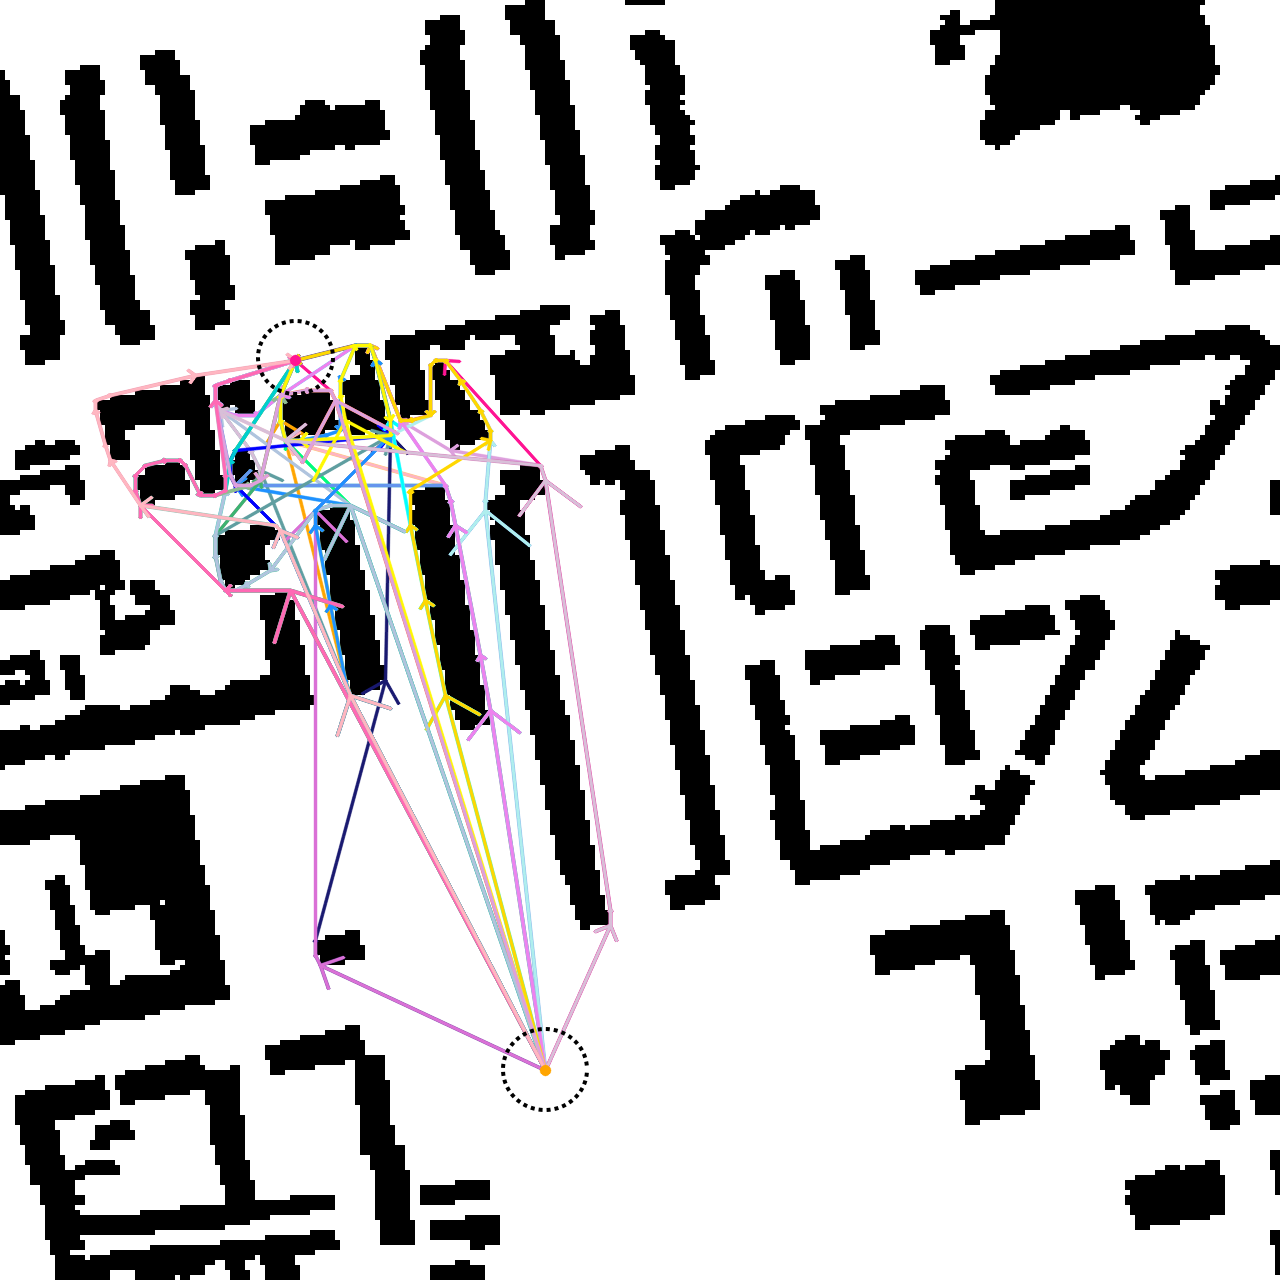
\includegraphics[width=4.2cm, cframe=gray .2mm]{50_RJ.png}}
  \centerline{A: 50 paths, in 3.7ms}
\end{minipage}
\hfill
\begin{minipage}{.48\linewidth}
  \centerline{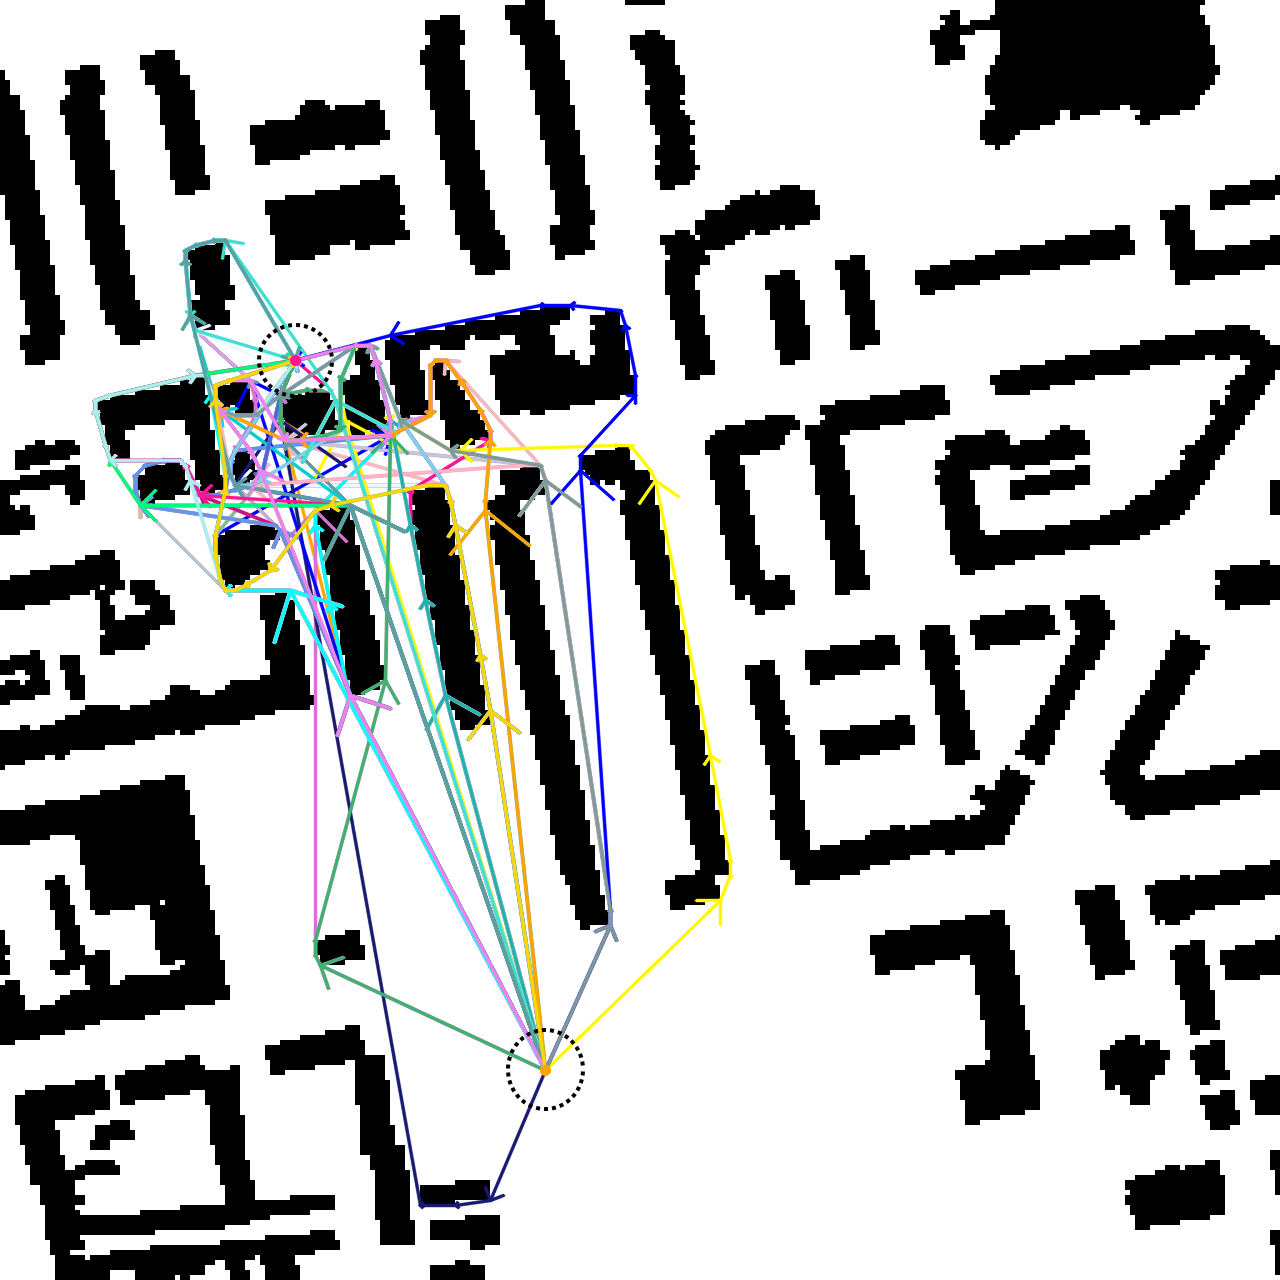
\includegraphics[width=4.2cm, cframe=gray 0.1mm]{100_RJ.png}}
  \centerline{B: 100 paths, in 8.2ms}
\end{minipage}
\vfill
\begin{minipage}{.48\linewidth}
  \centerline{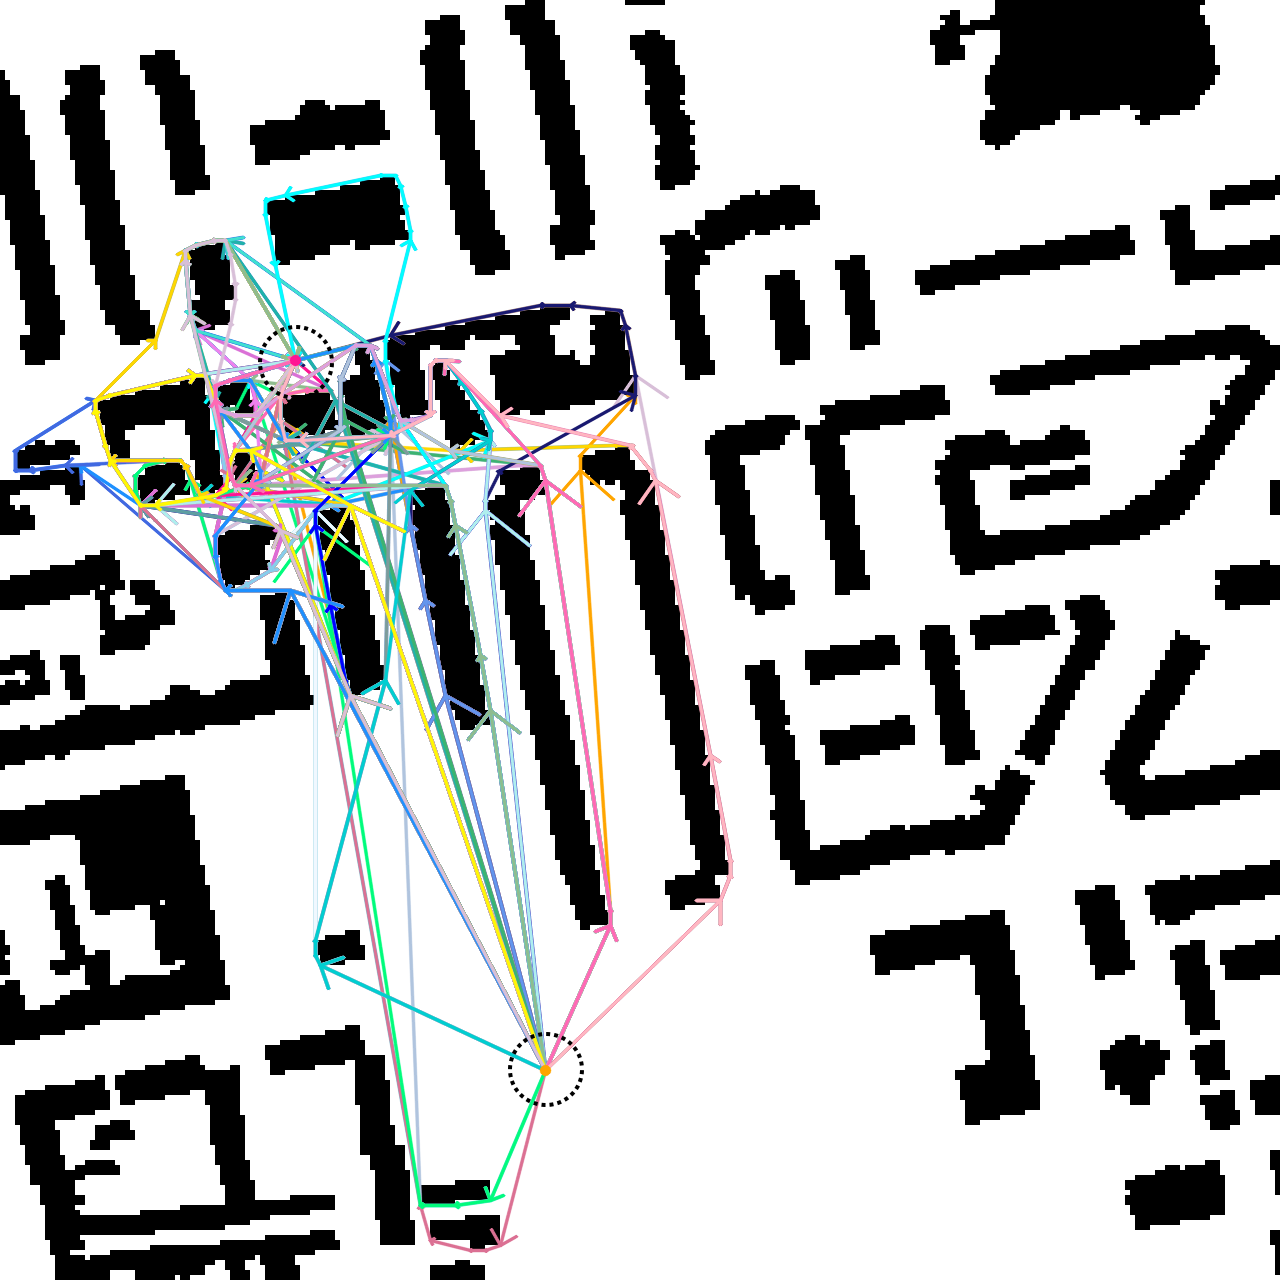
\includegraphics[width=4.2cm, cframe=gray 0.1mm]{200_RJ.png}}
  \centerline{C: 200 paths, in 16.2ms}
\end{minipage}
\hfill
\begin{minipage}{.48\linewidth}
  \centerline{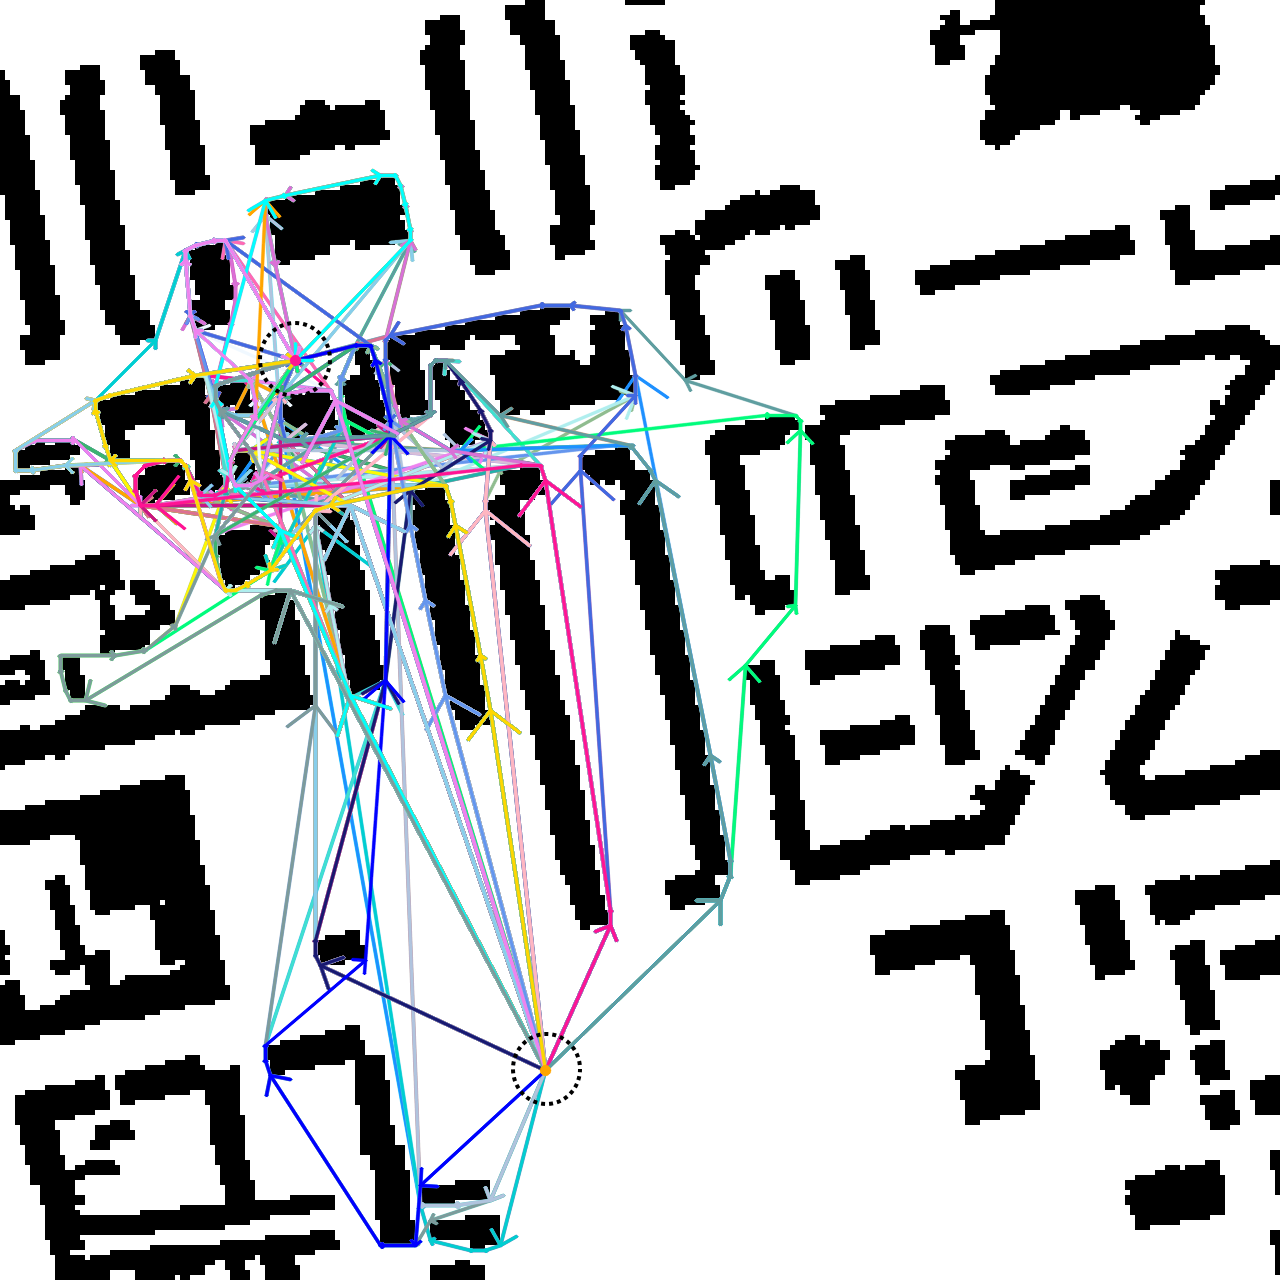
\includegraphics[width=4.2cm, cframe=gray 0.1mm]{400_RJ.png}}
  \centerline{D: 400 paths, in 38.1ms}
\end{minipage}
\vfill
\caption{These figures display multiple paths, with some of them partially overlapping, between the same start and target points, all determined by our method. The map employed is a 256x256 grid map ("Berlin\_1\_256" from the mentioned public map dataset). The start and target points, highlighted in pink and yellow, respectively, have coordinates (59, 72) and (109, 214), located at the center of circles. These experiments were conducted on a standard laptop running the Ubuntu operating system, equipped with a 3.2GHz CPU and 16GB of memory. Further details can be found in the Results section. }
\label{examples}
\end{figure}

However, several difficulties are encountered by existing works. Firstly, some of them require the use of H-signature\cite{bhattacharya2012search, bhattacharya2012topological} or similar indicators to determine whether two paths belong to the same topology. This results in an increase in time complexity as the number of paths to be considered grows, as it requires more calculations to determine if a new path and a previous path share the same topology. This results in an increase in time complexity as the number of paths to be considered grows, requiring more calculations to determine if a new path and a previous path share the same topology.

To address the limitations of H-signature\cite{bhattacharya2012search, bhattacharya2012topological} and similar indicators, Voronoi-based approaches\cite{kuderer2014online, palmieri2015fast} have been introduced. The distinctive property of Voronoi graph is that different sequences of Voronoi nodes inherently define topologically distinctive paths. While some of these methods have shown significant improvements in efficiency compared to algorithms that use H-signature. However, these methods still require a sequential search for topologically distinctive paths, one at a time.

To address the aforementioned issues, we propose a novel topologically distinctive path planning algorithm based on tangent graphs. This approach leverages the property that tangents form locally shortest paths, as discussed in previous works \cite{liu1991proposal, liu1992path, yao2019reinforcedrimjump}. Consequently, any two locally shortest paths inherently belong to different topologies. Our algorithm eliminates the need for indicators to determine path topology similarity and avoids the repetition of searches to obtain multiple paths. Instead, it retrieves all relevant paths in a single search, resulting in a significant improvement in efficiency when compared to existing methods. Additionally, we introduce a priority limitation mechanism to prevent the exponential growth of the queue size during graph search. The results demonstrate a remarkable enhancement in efficiency during the path planning process.A brief demonstration of our algorithm is presented in Fig. \ref{examples}.

The following sections of this article are organized as follows: Section \ref{RelatedWork} offers an introduction to relevant studies on distinctive topology path planning; section \ref{Methodology} provides a detailed description of the theory basis and key processes involved in our method; in Section \ref{Results}, we delve into the details of the construction of the tangent graph on the specified maps. Additionally, we present a comprehensive comparison between our method and several typical methods in terms of time cost, success rate and path length. This section also includes information about how our method performs as the number of paths increases and the scale of map increases; finally, in Section \ref{Conclusion}, we discuss the results obtained and potential drawbacks of the proposed method.

This letter contributes the following:

\begin{enumerate}
    \item A topologically distinctive path planning method based on the locally shortest property of tangents.
    \item The introduction of expansion reduction mechanism to mitigate the exponential growth of queue size in path planning that utilizes breadth-first search.
\end{enumerate}

\section{Related works}
\label{RelatedWork}

Two trajectories $\tau_1$ and $\tau_2$, connecting the same start and end coordinates, are considered homotopic if one can be continuously deformed into the other without intersecting any obstacles. Otherwise, they are considered topologically distinctive. Based on whether they introduce an explicit indicator, existing topologically distinctive path planning methods can be categorized into two types.

The first type introduces an explicit indicator to determine whether two paths belong to the same topology, typically in relation to obstacles.

H-signature, proposed by Subhrajit Bhattacharya for 2-dimensional maps, is an indicator computed using the Cauchy integral theorem and the Residue theorem from complex analysis. It is defined as the integration of an ``obstacle marker function" along a path, where the obstacle marker function involves the representative point of each obstacle. Bhattacharya's work, as seen in references \cite{bhattacharya2010search, kim2012optimal, bhattacharya2012topological}, extends H-signature to 2D maps and later to 3D maps \cite{bhattacharya2012search}. Two paths share the same H-signature if and only if they belong to the same topology; otherwise, they do not. Combining the H-signature constraint with standard graph search algorithms like A*, these methods find multiple topologically distinctive paths by repeating graph searches multiple times. 

However, H-signature's efficiency is affected by several factors: 1, the more obstacles there are, the more calculations are needed to compute the H-signature of a path; 2, as the number of paths increases, the average time required to compute a single path increases linearly, as each path needs to be compared with the H-signature of existing paths, and the number of existing paths grows. In contrast, our method does not need an explicit indicator to distinguish whether two paths belong to the same topology. As a result the average time required to compute a single path is increase very slowly as total number of path increases.

Markus Kuderer \cite{kuderer2014online} introduced the concept of the winding angle of a trajectory, defined as the sum of infinitesimal angle differences to the representative points of obstacles along the trajectory. Similar to H-signature, paths belonging to the same topology have the same winding angle, while those with distinctive topologies do not.

To address the issue of multiple paths to the goal within the same homotopy class when using H-signature with A*, Kuderer and colleagues incorporated Voronoi graphs to ensure that each path corresponds to a unique homotopy class. Their results, as presented in \cite{kuderer2014online}, showed a significant improvement in efficiency compared to using H-signature combined with A*. In comparing to the Voronoi graph, our method generate locally shortest paths, which are shorter than the paths produced by Voronoi graphs in terms of path length. Our method utilizes tangent graph\cite{liu1991proposal, oh2017edge} to generates locally shortest paths.    

TARRT* (Topology-Aware RRT*), as proposed by Yi et al. in \cite{yi2017topology}, introduces a method for determining the homotopic equivalence of two arbitrary paths based on properties of strings recognized by a Deterministic Finite Automaton (DFA). These strings also involve the representative point of each obstacle, with the condition that no point is allowed to lie on any line connecting any two other representative points. 

Specifically, non-obstacle regions are divided into a set of subregions by lines that intersect representative points, and the connections between these subregions are referred to as reference frames. TARRT* assigns a unique label to each reference frame and appends the label of the reference frames to the string whenever the path crosses them. This string-based approach appears to be more efficient than H-signature because its calculation doesn't involve all obstacle representative points. However, TARRT* shares a limitation with normal RRT (Rapidly Exploring Random Trees) in that they are both probabilistically complete methods for finding existing solutions. For instance, they may fail when the path must pass through a narrow, long opening in an obstacle.

In constrast, our method use a tangent graph to determine all topologically distinctive path, which is complete in determining all possible solutions rather than probabilistic in determining all solutions.


The second type of methods does not rely on an explicit topology indicator. 

As previously noted, path segments in the Voronoi graph are inherently unique between two obstacles, ensuring that different paths found in the Voronoi graph guarantee distinctive topology. Consequently, the Voronoi graph is widely employed in distinctive topological path planning.

Luigi Palmieri \cite{palmieri2015fast} introduced the Randomized Homotopy Classes Finder (RHCF), a fast randomized method that identifies a set of K paths lying in distinct homotopy classes using the Voronoi graph. The approach involves repeatedly searching for random paths in the Voronoi graph and saving them if they differ from all previous paths. The process stops when K different paths have been found. In their results, RHCF outperformed Yen's K shortest path finding method \cite{yen1971finding} in terms of speed.

As well as \cite{kuderer2014online}, Voronoi graph generate path that far from locally shortest paths, while our method use tangent graph to generate locally shortest path. Additionally, RHCF's mean time cost of search path increase as total number of path increases (more comparison between paths ), while our method's average time required to compute a single path is increases very slowly as total number of path increases.

In contrast to mobile robots, which require determining the optimal joint path in the task space, J.J. Rice \cite{rice2020multi} proposed a bifurcation branch algorithm to characterize the solution space with the bifurcation branch roadmap. This approach generates initial joint paths that identify all homotopy classes and locally optimal paths in all relevant homotopy classes with the lowest cost, which is very likely the globally optimal path. While this method is more capable than traditional approaches in finding the global optimal path, it faces challenges as the number of homotopy classes grows exponentially with the complexity of the solution space. This presents significant difficulties when extending it to topologically distinctive path planning for mobile robots.

In constrast, our method can adapt to complex grid maps, as the exponentially growth of number of homotopy classes is limited by the limitation of queue size during Breadth First Search. 


\section{Methodology}
\label{Methodology}

\subsection{Theory basis}

In this section, we aim to establish the relationship between topologically distinct paths and locally shortest paths. We begin by providing clear definitions for locally shortest paths and topologically distinctive paths. Subsequently, we prove the relationship between these two concepts. It is essential to note that all paths discussed herein share the same start and target points.
\begin{myDef}
A path $p$ is considered a locally shortest path if, within any small region along its trajectory, it is impossible to find a shorter collision-free path than $p$ \cite{131594}.
\end{myDef}

\begin{myDef}
Two trajectories (or paths), $\tau_1$ and $\tau_2$, are said to belong to the same homotopy class if one can be smoothly deformed into the other without intersecting obstacles; otherwise, they belong to different homotopy classes \cite{bhattacharya2010search}.
\end{myDef}

\begin{myTheo}
Any two locally shortest paths that share the same start and target cannot belong to the same homotopy class.
\end{myTheo}

\begin{myProof}
Assuming two locally shortest paths ($p_1$ and $p_2$) are in the same homotopy class implies that one of them (assume $p_1$) can be transformed consistently into the other ($p_2$) without intersecting obstacles. However, during this transformation from $p_1$ to $p_2$, the length of the path increases monotonically. This contradicts the definition of a locally shortest path, which is the shortest path within its local neighborhood. Therefore, any nearby path to $p_2$ should be longer than $p_2$.
\end{myProof}

Building upon this theoretical foundation, if multiple locally shortest paths exist, we consequently obtain multiple topologically distinctive paths.

\begin{myTheo}
Locally shortest paths can be formed by tangents connecting the start and target points.
\end{myTheo}

\begin{myProof}
This has been established in previous work \cite{131594, oh2017edge, yao2019reinforcedrimjump}.
\end{myProof}

%In addition to its advantage of forming locally shortest paths, the tangent graph also yields the shortest paths.

Therefore, utilizing the tangent graph allows for the generation of multiple topologically distinctive paths. Importantly, the time cost of tangent graph detection remains insensitive to the scale increase of maps, as the tangent graph is solely determined by the geometric elements of the maps. These advantages will be demonstrated and discussed in Section \ref{Results}.


\subsection{Algorithm}

Building upon the theoretical foundation, we can extract multiple topologically distinctive paths from the tangent graph. In this section, our focus shifts to the efficient utilization of this graph to obtain multiple topologically distinctive paths. Traditionally, two well-known methods for determining paths between two nodes in a graph are Breadth-First Search (BFS) and Best-First Search. Given that existing methods (refer to Section \ref{RelatedWork} for more details) often require multiple searches to obtain multiple paths, our objective is to find multiple paths in a single graph search. Consequently, we choose to implement our method based on Breadth-First Search. However, due to the specialized nature of searching for topologically distinctive paths, certain modifications are necessary.

\subsubsection{Loop avoidance}

As a fundamental principle in topologically distinctive paths \cite{bhattacharya2012topological}, path planning with distinctive topology strictly avoids the presence of loops. Loops in this context can take two forms: either a waypoint is revisited within a single path, or the path intersects with itself. It is crucial to consider these scenarios when attempting to find multiple paths. Notably, as the number of waypoints in a path increases, the time required for loop detection also grows. Experimental results demonstrate that the ratio of loop avoidance in the overall time cost increases proportionally with the required number of paths.

\subsubsection{Path search} 



\begin{algorithm}[t] 
 \normalem
\label{a1}
  \caption{Topology-aware Breadth First Search}
  \KwIn{$g_s, g_t, G(V, E), K$}  
  \KwOut{$P$}
  $P = \{g_s\}, P' = \emptyset, P_f = \emptyset$; \\
  add $g_s$ and $g_t$ to $G$; \\
  \While{find no $K$ paths and $P$ is not empty} {
  	 $P' = \emptyset$; \\
     \For{each unfinished path $p$ in $P$} {
     	\For{each nodes $v$ of $G$ that connect to last nodes of $p$}{
     	$p'$ = add $v$ to $p$; \\
     	\If{$p'$ have no loops and $p'$ meet taut condition}{
     	\eIf{$p'$ reach $g_t$} {
     	add $p'$ to $P'$; \\
     	}{
     	add $p'$ to $P_f$; \\
     	}
     	}
     	}	
     }
     $P = P'$ ; \\		  
  } 
  return $P_f$;
\end{algorithm}

\begin{table}[t]
	\centering  % 显示位置为中间
	\caption{Table of notations}  % 表格标题
	\label{table_of_notation}  % 用于索引表格的标签
	%字母的个数对应列数,|代表分割线
	% l代表左对齐,c代表居中,r代表右对齐
	\begin{tabular}{|c|c|c|c|}  
		\hline 
		%& & & \\[-6pt]  %可以避免文字偏上来调整文字与上边界的距离
		Name & Meanning & Name & Meanning \\  
		\hline
		$g_s$   & start point & $g_t$ & target point \\
		\hline
		$P, P'$ & set of unfinished path & $P_f$ & set of finished path \\
		\hline		
		$G(V, E)$ & tangent graph & $v$ & a node in tangent graph \\
		\hline		
		$p, p'$ & path & $P_B$ & \makecell[c]{set of unifinished path \\ (backup queue)} \\
		\hline
		%\hline
	\end{tabular}
\end{table}

Our method comprises two key components: tangent graph detection and path search. Tangent graph detection from grid maps is a well-explored area, and there exist established methods for this purpose \cite{131594, yao2019reinforcedrimjump, oh2017edge}. Consequently, our primary focus in this manuscript lies in the efficient search for paths.

To leverage the efficiency of line-of-sight scans \cite{oh2017edge}, we adopt the ENL-SVG method \cite{oh2017edge} to generate the tangent graph. To avoid redundant tangent graph computations for the same map, we store the tangent graph in files. Ensuring that all paths are locally shortest, we incorporate the taut condition \cite{oh2017edge} during the path search.

We have modified the classical Breadth-First Search (BFS) algorithm to search for multiple topologically distinctive paths, as outlined in Algorithm \ref{a1}. The notation used in the pseudocode is detailed in Table \ref{table_of_notation}.

\begin{algorithm}[t] 
 \normalem
\label{a2}
  \caption{Topology-aware Breadth First Search with expansion reduction}
  \KwIn{$g_s, g_t, G(V, E), K$}  
  \KwOut{$P$}
  $P = \{g_s\}, P' = \emptyset, P_f = \emptyset, $\hl{$P_B = \emptyset$}; \\
  add $g_s$ and $g_t$ to $G$; \\
  \While{$P_f$ have no $K$ paths and $P$ is not empty} {
     $P' = \emptyset$; \\
     \For{each unfinished path $p$ in $P$} {
     	\For{each nodes $v$ of $G$ that connect to last nodes of $p$}{
     	$p'$ = add $v$ to $p$; \\
     	\If{$p'$ have no loops and $p'$ meet taut condition}{
     	\eIf{$p'$ reach $g_t$} {
     	add $p'$ to $P'$; \\
     	} {
     	add $p'$ to $P_f$; \\
     	}
     	}
     	}	
     }
     \hl{$P = \emptyset$;} \\
     \hl{sort $P'$ in increasing heurstic value;} \\
     \hl{move top $K$ path of $P'$ to $P$ and move remaining path in $P'$ to $P_B$;} \\
     \hl{sort $P_B$ in increasing heurstic value;} \\
     \If{\hl{$P$ have no $K$ paths}} {
	  \While{\hl{$P_B$ is not empty and $P$ have no $K$ path}} {
	  \hl{move path with minimum heurstic value in $P_B$ to $P$;} \\	  
	  }     
     }		  		  
  } 
  return $P_f$;
\end{algorithm}


\subsubsection{Expansion reduction}    
One drawback of Algorithm \ref{a1} is the exponential growth in the size of unfinished paths as the number of expansions increases. To address this issue, we propose an expansion reduction technique to mitigate the exponential growth during iterations of BFS. This technique involves splitting the queue into two: a priority queue and a backup queue.

Assuming the required number of paths is denoted as $K$, in each iteration of BFS, we select the top $K$ paths with the minimal heuristic value (calculated in the same manner as A*) and store them in the priority queue as candidates for expansion. The remaining unfinished paths are cached in a backup queue, sorted by their heuristic values.

If there are fewer than $K$ unfinished paths in the priority queue, we extract unfinished paths from the backup queue and insert them into the priority queue until there are $K$ elements in the priority queue or the backup queue is empty, as shown in Algorithm \ref{a2}. The relevant code related to the priority queue has been highlighted.

Essentially, this approach changes the order of expansion of unfinished paths, prioritizing paths that are closer to the target (i.e., have lower heuristic values). As a result, the path search concludes sooner compared to the scenario without expansion reduction. Importantly, the expansion reduction does not compromise completeness. Algorithm \ref{a2} outlines BFS with expansion reduction, specifying its differences compared to Algorithm \ref{a1}.

An illustrative example highlighting the benefits of introducing expansion limitation is presented in Fig. \ref{priority}. The map used for this comparison is Berlin\_1\_256.map from the public grid map dataset mentioned earlier, with the start and target points set at (59, 72) and (109, 214), respectively.


\begin{figure*}[t]
\centering
\vspace*{8pt}
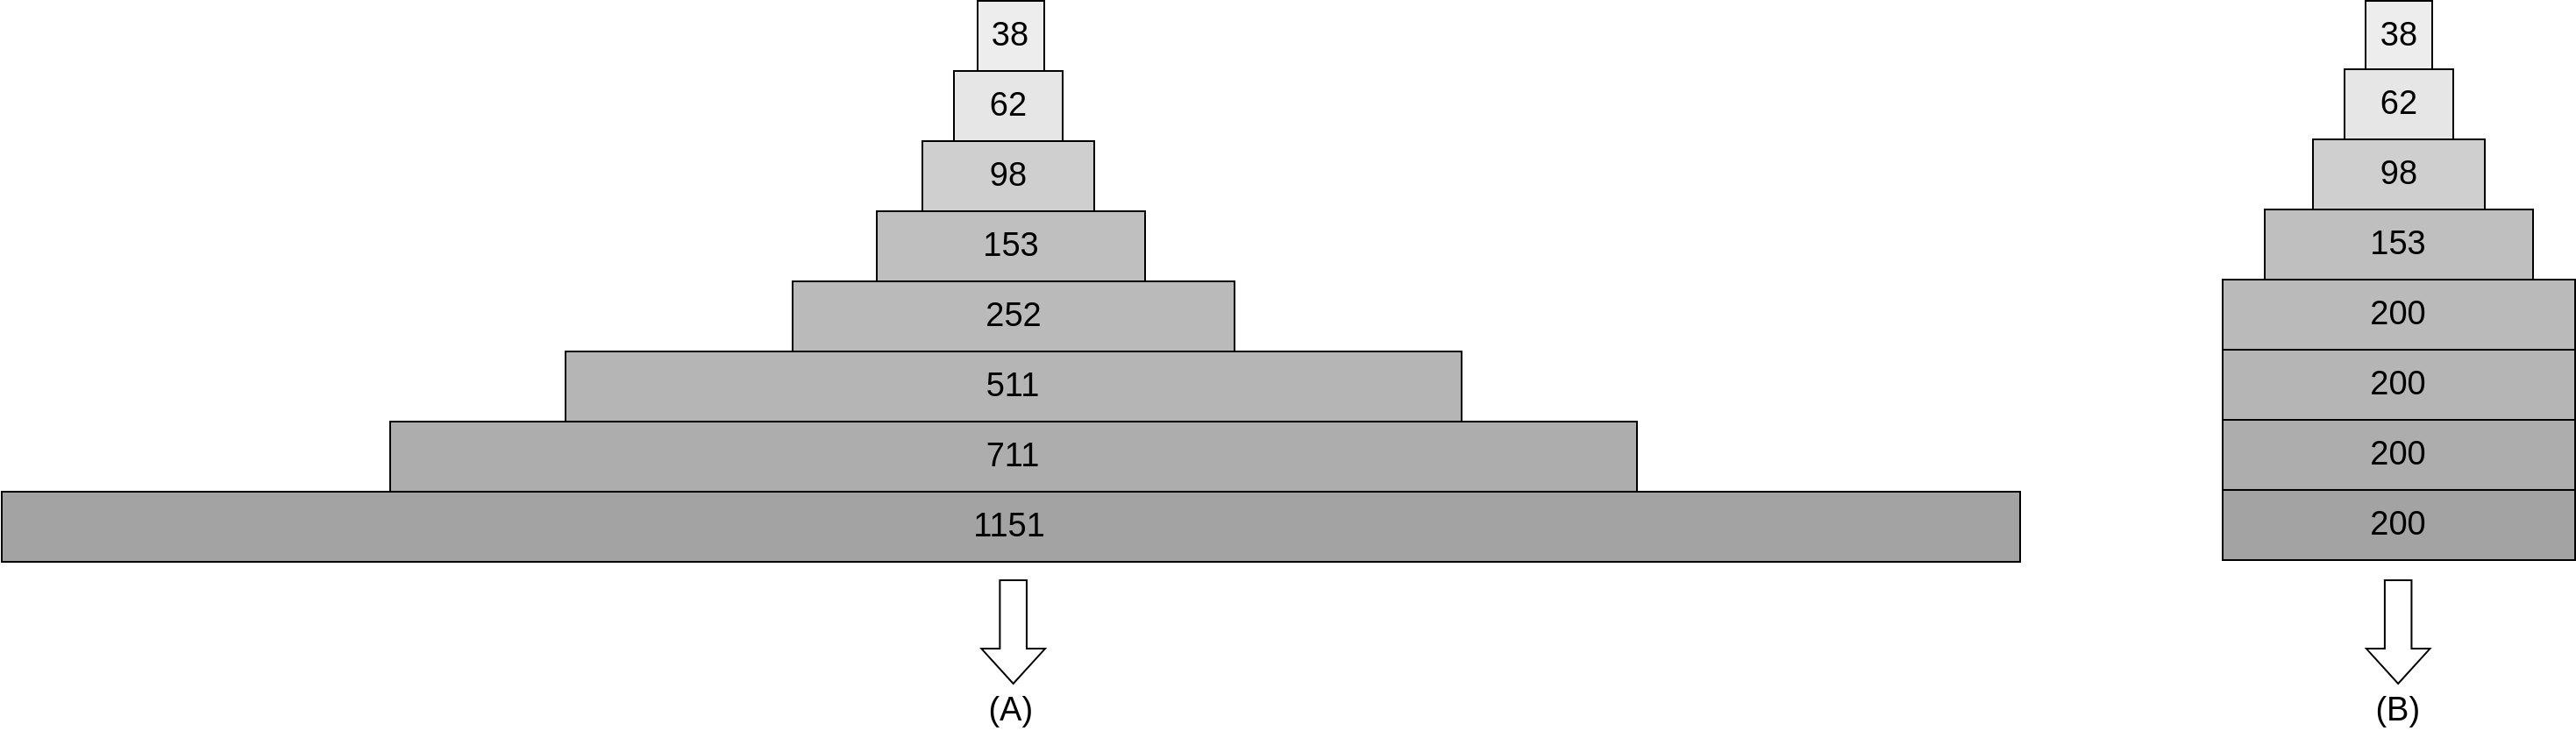
\includegraphics[width=12.5cm]{priority.png}
\caption{These figures depict the changes in queue size during BFS expansion before (Fig A) and after (Fig B) implementing expansion reduction in the same scenario (Fig. \ref{examples}), where the goal is to find 200 paths. In both Figures A and B, it's evident that the queue size grows exponentially before the introduction of priority limitation, but stabilizes once it reaches 200 after implementing this enhancement. Consequently, obtaining 200 paths takes 48.5ms before the introduction of priority limitation, while it only takes 16.8ms afterward.
} 
\label{priority}
\end{figure*}



\begin{figure}[t] \scriptsize
%\begin{tabular}{cc}
\begin{minipage}{.24\linewidth}
  \centerline{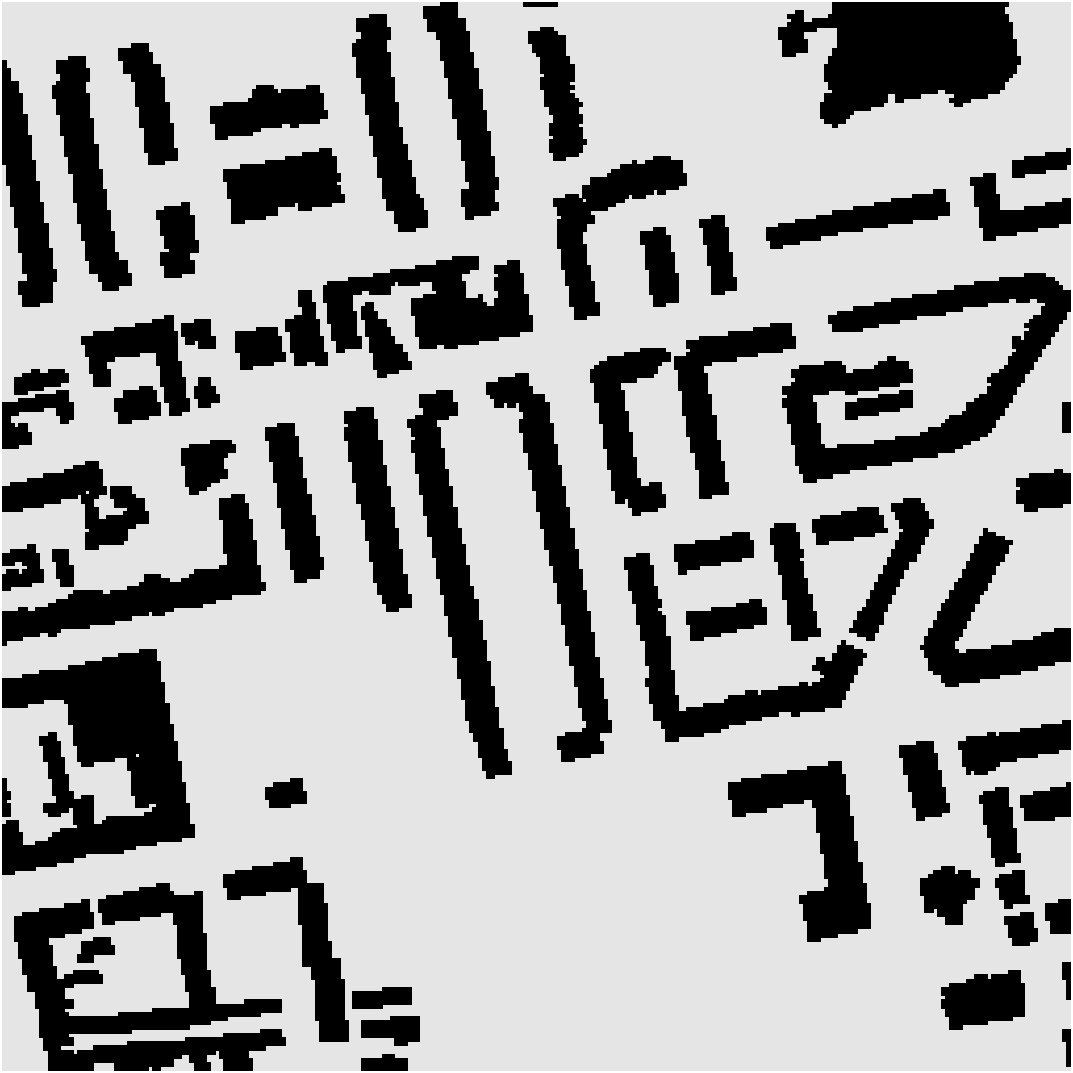
\includegraphics[width=2.1cm]{Berlin_1_256.png}}
  \centerline{A: Berlin\_1\_256}
\end{minipage}
\hfill
\begin{minipage}{.24\linewidth}
  \centerline{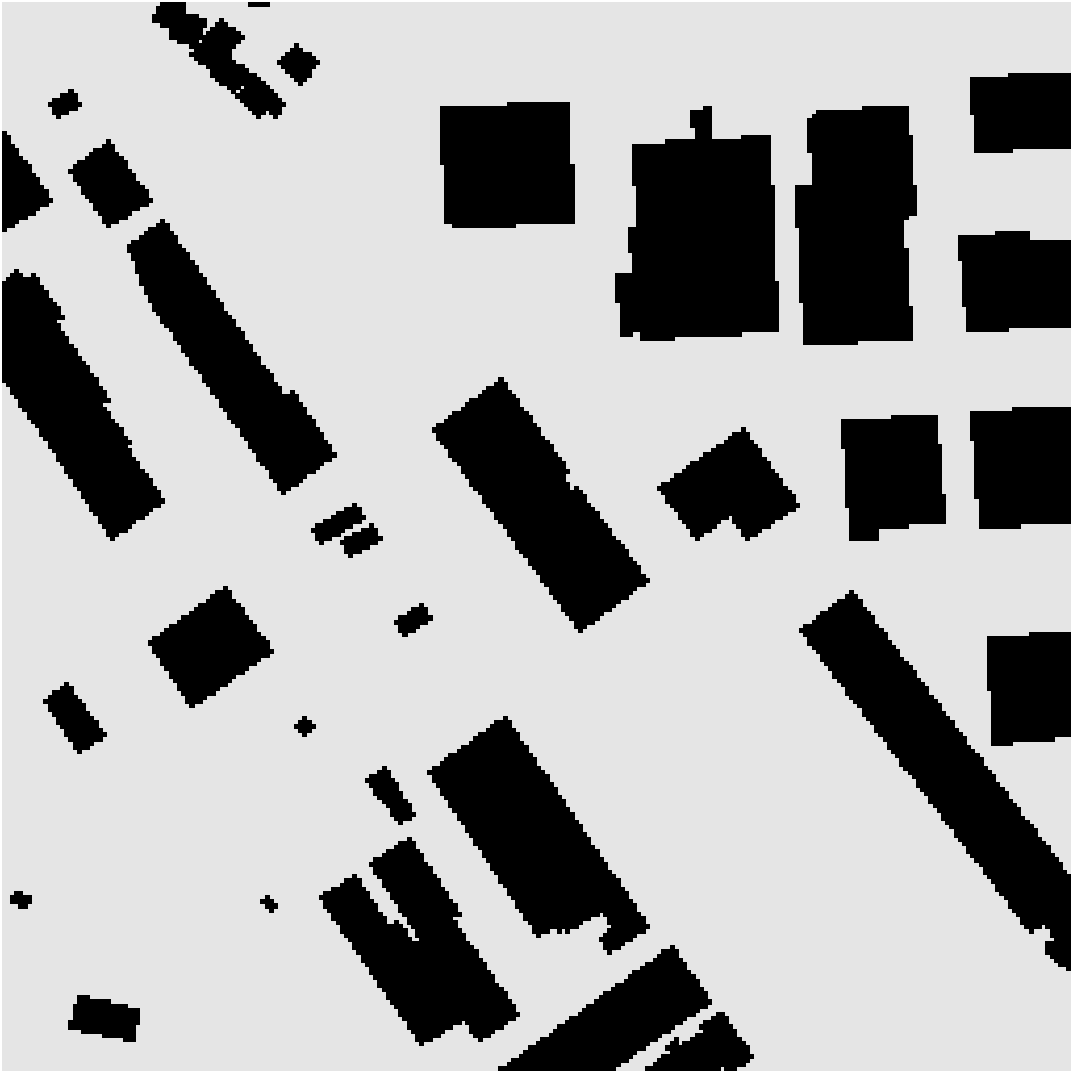
\includegraphics[width=2.1cm]{Boston_2_256.png}}
  \centerline{B: Boston\_2\_256}
\end{minipage}
\hfill
\begin{minipage}{.24\linewidth}
  \centerline{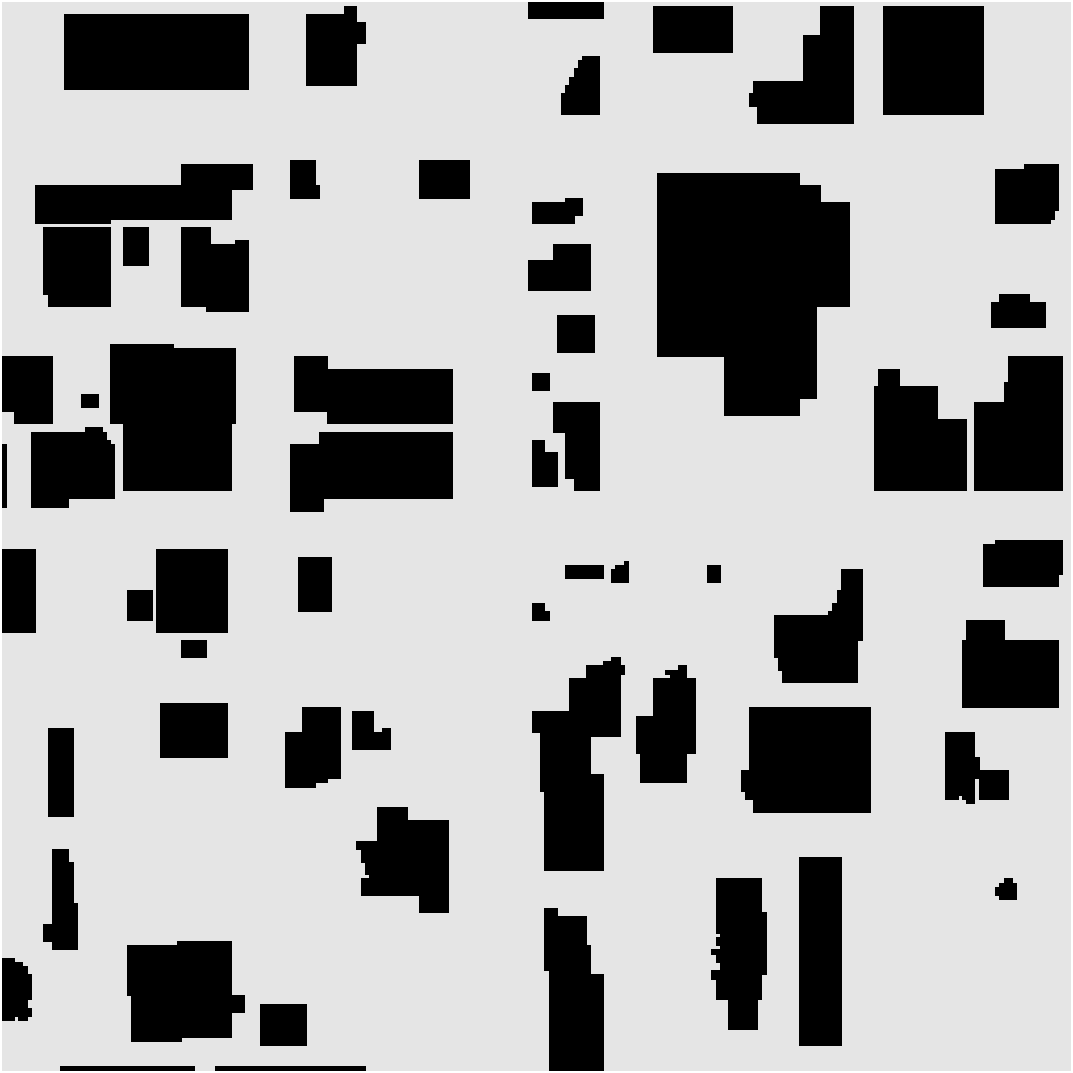
\includegraphics[width=2.1cm]{Denver_2_256.png}}
  \centerline{C: Denver\_2\_256}
\end{minipage}
\hfill
\begin{minipage}{.24\linewidth}
  \centerline{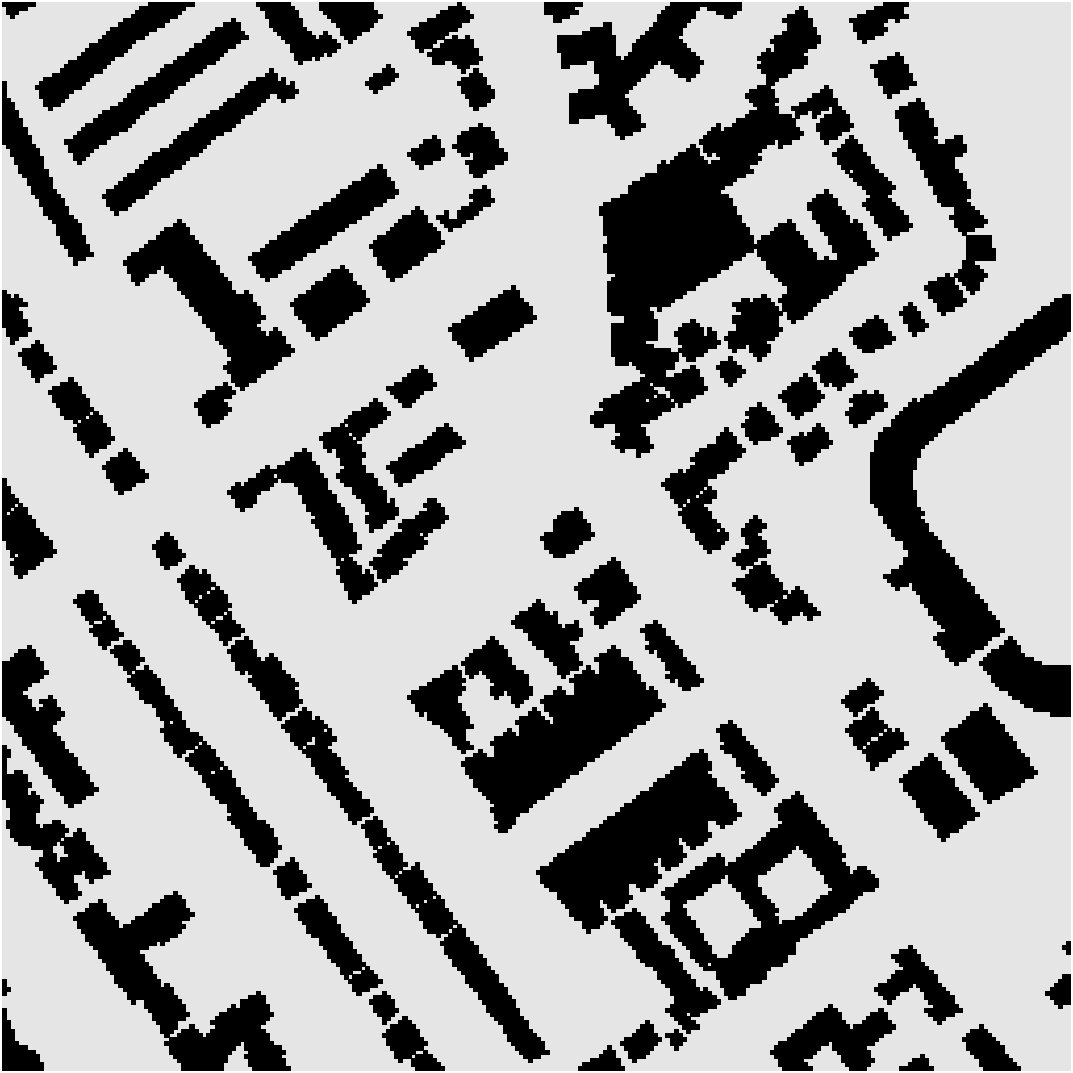
\includegraphics[width=2.1cm]{London_2_256.png}}
  \centerline{D: London\_2\_256}
\end{minipage}
\vfill
\vspace{0.2cm}
\begin{minipage}{.24\linewidth}
  \centerline{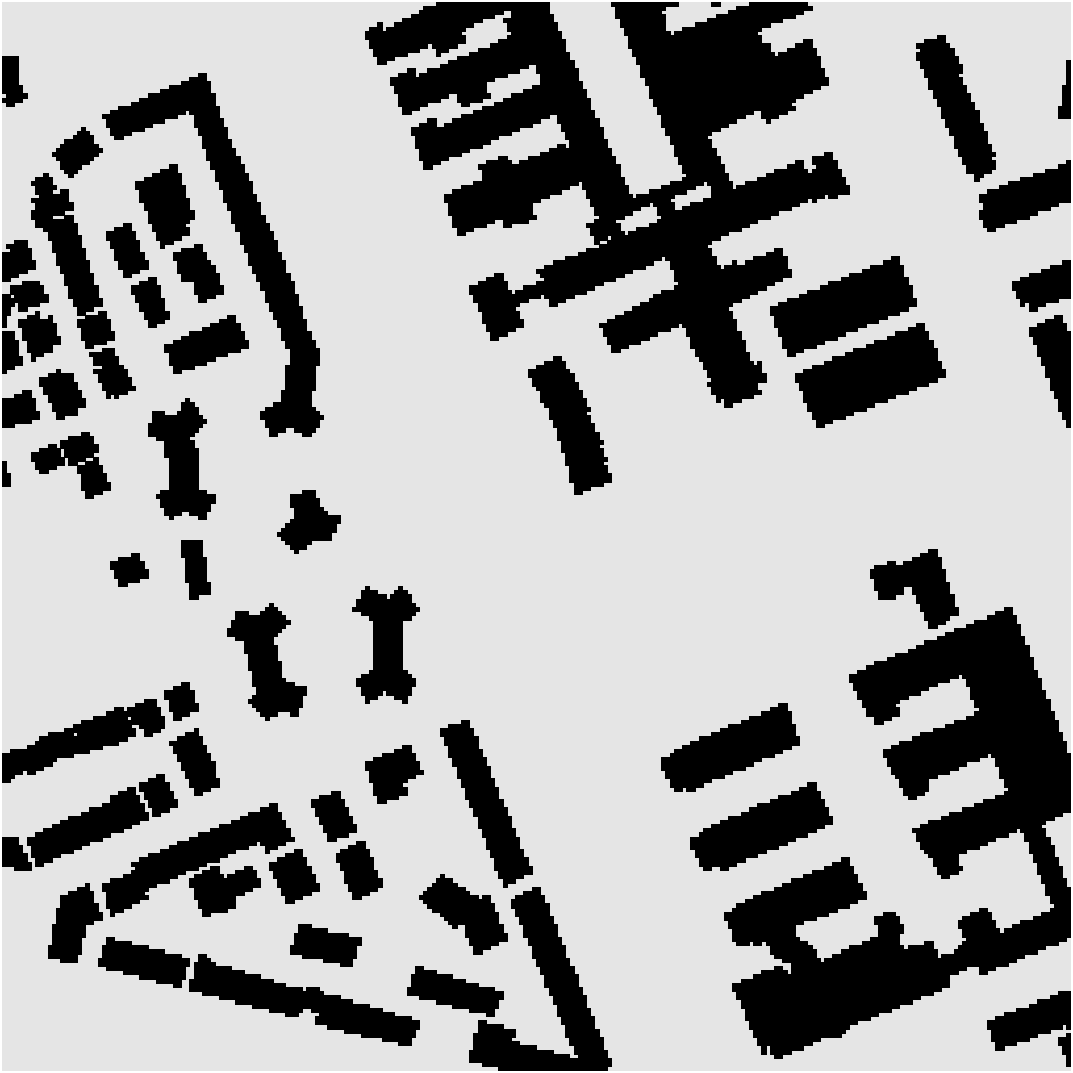
\includegraphics[width=2.1cm]{Milan_2_256.png}}
  \centerline{E: Milan\_2\_256}
\end{minipage}
\hfill
\begin{minipage}{.24\linewidth}
  \centerline{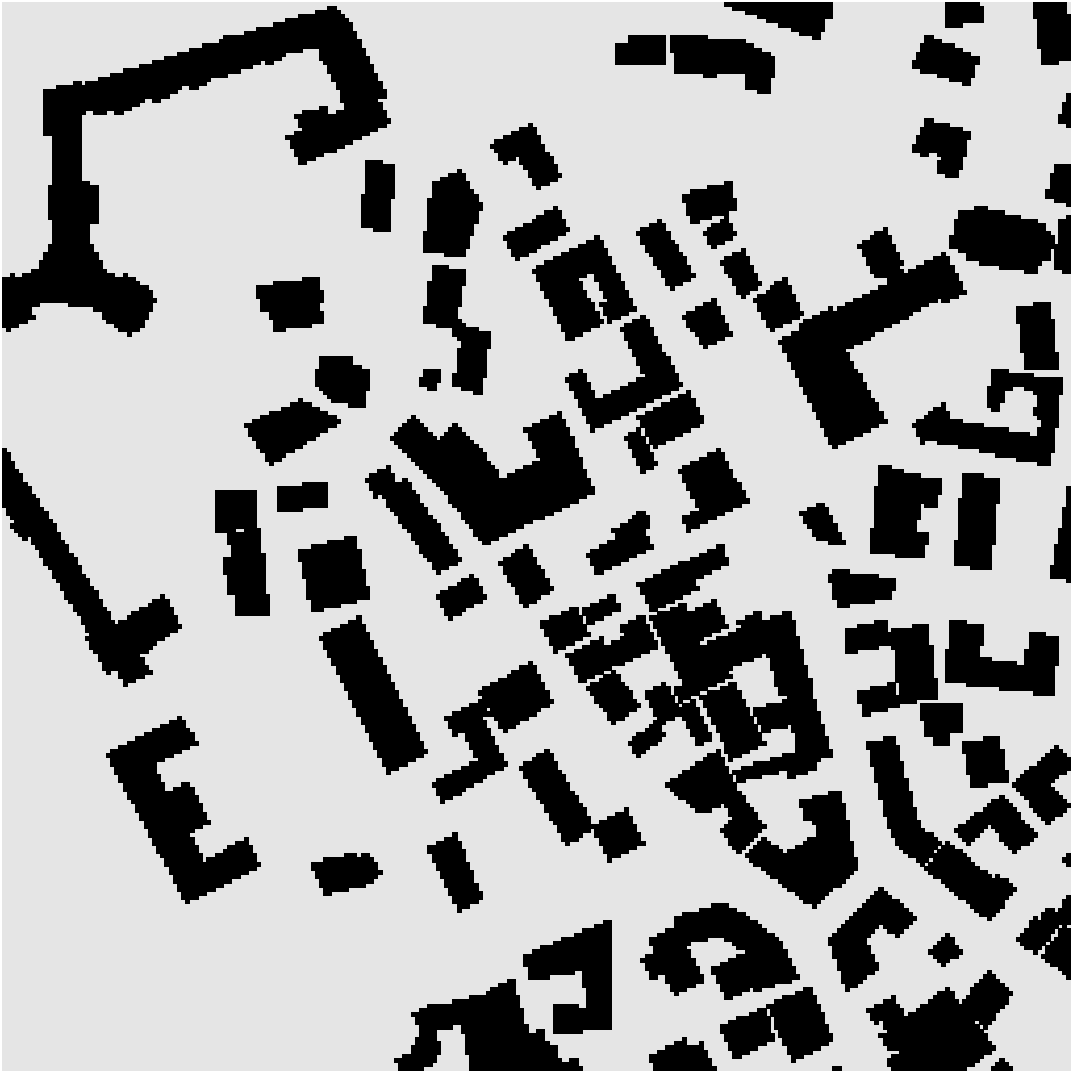
\includegraphics[width=2.1cm]{Moscow_2_256.png}}
  \centerline{F: Moscow\_2\_256}
\end{minipage}
\hfill
\begin{minipage}{.24\linewidth}
  \centerline{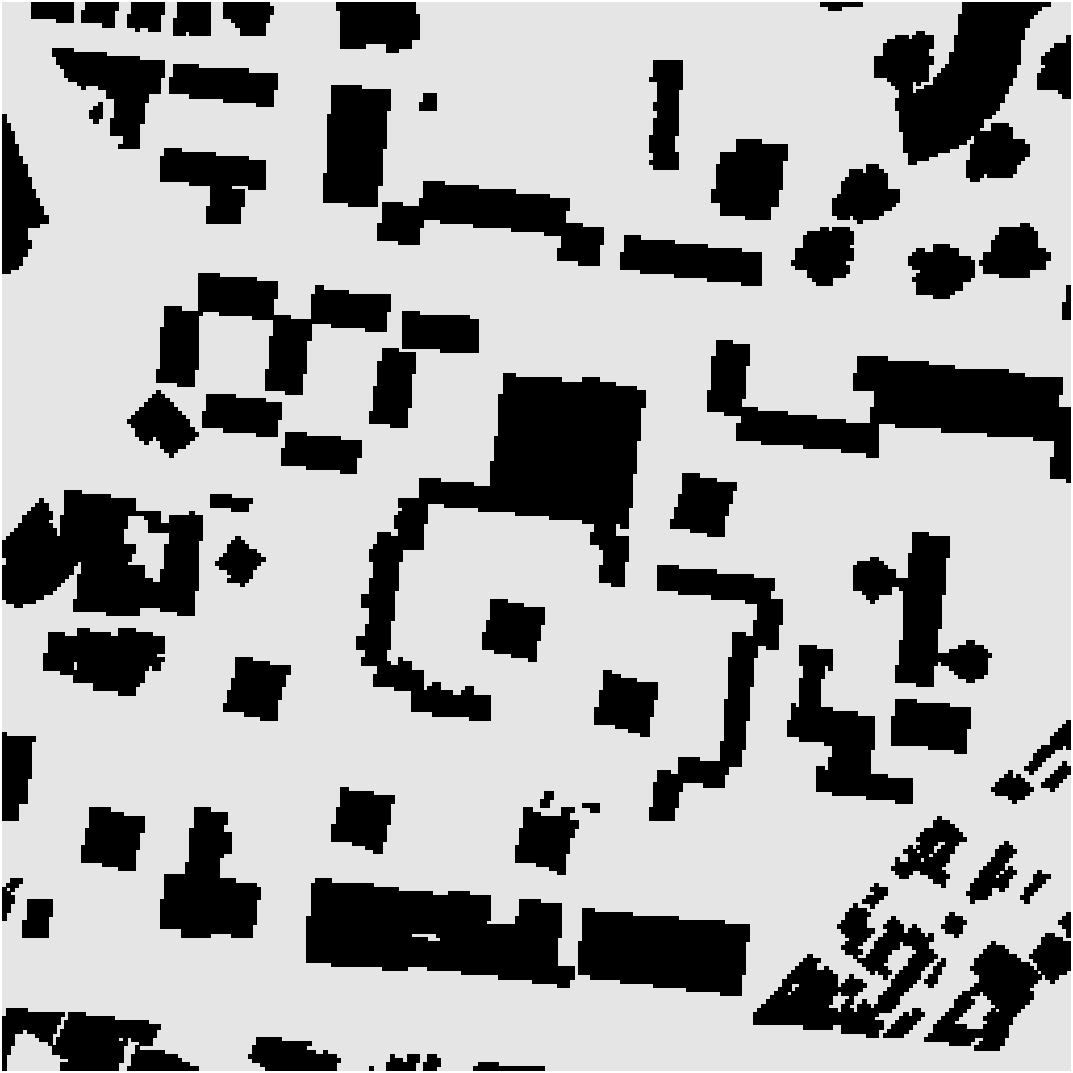
\includegraphics[width=2.1cm]{Paris_0_256.png}}
  \centerline{G: Paris\_0\_256}
\end{minipage}
\hfill
\begin{minipage}{.24\linewidth}
  \centerline{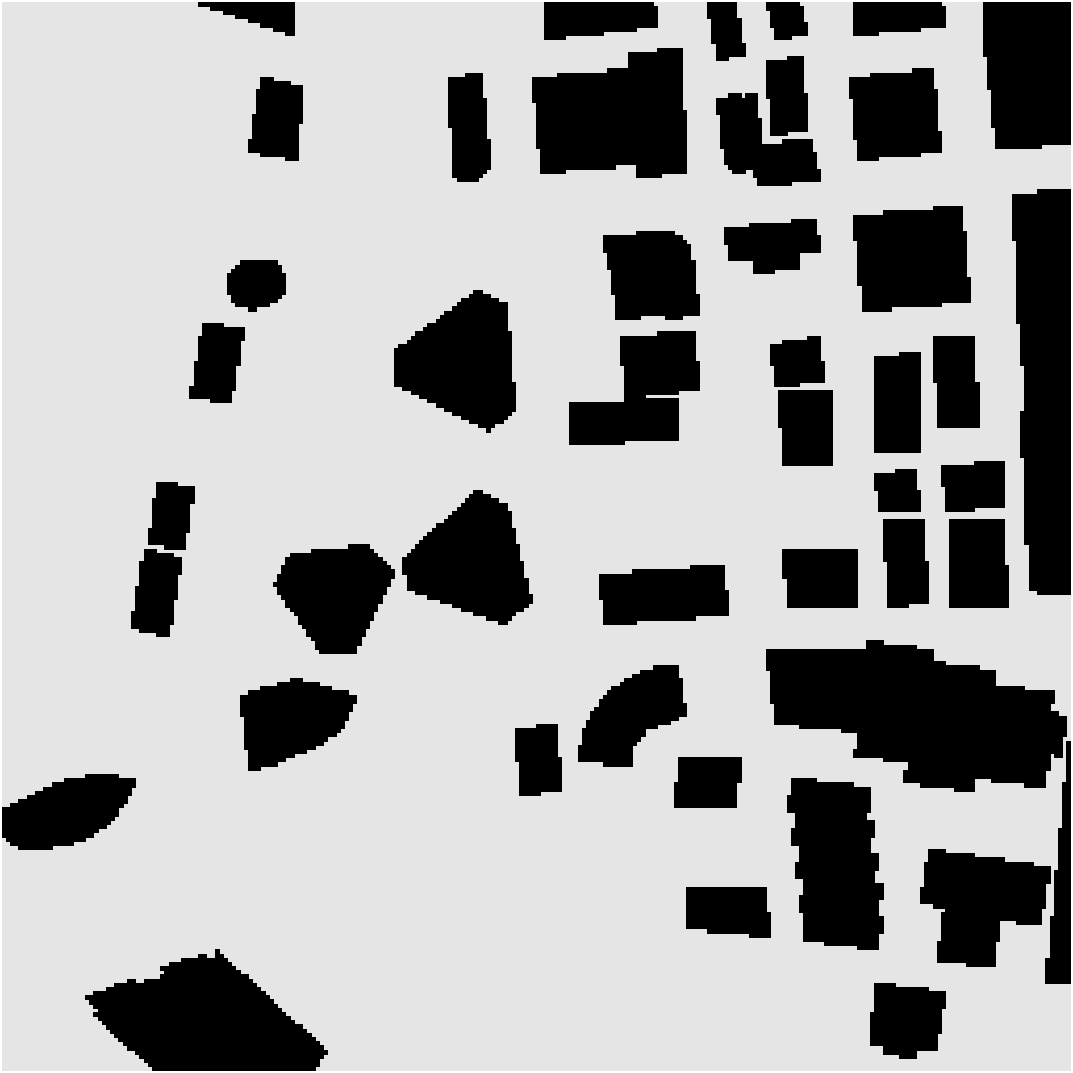
\includegraphics[width=2.1cm]{Sydney_1_256.png}}
  \centerline{H: Sydney\_1\_256}
\end{minipage}
\vfill

\caption{These figures showcase eight grid maps from \cite{sturtevant2012benchmarks} utilized in the comparison with other algorithms. The size of each map is 256$\times$256.}
\label{city_maps}
\end{figure}

\section{Results}
\label{Results}
%In this section, we provide more detailed insights into the performance of our algorithm and compare it with other distinctive topology path planning methods. In the first subsection, we elaborate on the construction of the tangent graph. To ensure a fair comparison, we use the implementations provided by the respective authors. We compare our method with HA*, HTheta*, and RHCF in terms of the time cost as the required number of paths and scale of map increases. We also compared path length of each method. HA* and HTheta* are H-signature-based algorithms\footnote{https://github.com/subh83/DOSL}, while RHCF is a Voronoi graph-based algorithm\footnote{https://github.com/srl-freiburg/srl\_rhcf\_planner}.

%Our experiments are conducted using a well-known grid map dataset\cite{sturtevant2012benchmarks}\footnote{https://movingai.com/benchmarks/grids.html}. To obtain more distinctive topology paths, we select city maps from the dataset, as illustrated in Fig. \ref{city_maps}. Because city maps contain lots of obstacles, so it is feasible to find hundreds topologically distinctive paths, all method have enough space to demostrate their capability. For each map, we randomly sample 100 start and target combinations as inputs for path planning. To study how methods' performance changes as scale of map increasing, we magnify raw map to get multiple larger maps. The manification of maps range from 1.0 to 4.0 (including 1.0, 1.1, 1.2, 1.3, 1.4, 1.5, 1.8, 2.0, 2.5, 3.0, 3.5, 4.0 specifically), so the scale of map ranges from 256*256 to 1024*1024. The experiments were carried out on a laptop running Ubuntu 20.04, equipped with a Ryzen 7 5800h (3.2GHz) CPU and 16GB of memory. 

%To demostrate the capability of methods to find huge amount of topologically distinctive paths, we set all methods to find 10 ~ 400 (including 10, 20, 30, 40, 50, 80, 120, 160, 200, 250, 300, 350, 400 specifically) paths. For HA* and HTheta*, their success rate decreas to less than 10\% when try to find 200 tipologically distinctive paths, so we set the maximum number of required paths for them to 200, to reduce the total time cost of experiment. 

In this section, we delve into a detailed examination of our algorithm's performance, comparing it with other distinctive topology path planning methods. The first subsection provides insights into the construction of the tangent graph. To ensure a fair comparison, we utilize the implementations provided by the respective authors. Our method is compared with HA*, HTheta*, and RHCF, focusing on the time cost as the required number of paths and the scale of the map increases. Path length comparisons for each method are also conducted. HA* and HTheta* are H-signature-based algorithms \footnote{https://github.com/subh83/DOSL}, while RHCF is a Voronoi graph-based algorithm \footnote{https://github.com/srl-freiburg/srl\_rhcf\_planner}.

The experiments are conducted using a well-known grid map dataset \cite{sturtevant2012benchmarks} \footnote{https://movingai.com/benchmarks/grids.html}. City maps from the dataset are selected for their high obstacle density, allowing the generation of hundreds of topologically distinctive paths, providing ample space for each method to demonstrate its capability. For each map, 100 start and target combinations are randomly sampled as inputs for path planning. To study how method performance changes with an increasing map scale, raw maps are magnified to create larger maps. The magnification ranges from 1.0 to 4.0 (including 1.0, 1.1, 1.2, 1.3, 1.4, 1.5, 1.8, 2.0, 2.5, 3.0, 3.5, 4.0 specifically), resulting in map scales from 256$\times$256 to 1024$\times$1024. Experiments were conducted on a laptop running Ubuntu 20.04, equipped with a Ryzen 7 5800h (3.2GHz) CPU and 16GB of memory.

To showcase the methods' capability to find a substantial number of topologically distinctive paths, we set all methods to find paths ranging from 10 to 400 (including 10, 20, 30, 40, 50, 80, 120, 160, 200, 250, 300, 350, 400 specifically). For HA* and HTheta*, their success rate drops to less than 10\% when attempting to find 200 topologically distinctive paths, so we set the maximum number of required paths for them to 200 to reduce the overall time cost of the experiment.


\subsection{Construction of tangent graph}

\begin{figure}[t] \scriptsize
%\begin{tabular}{cc}
\begin{minipage}{.48\linewidth}
  \centerline{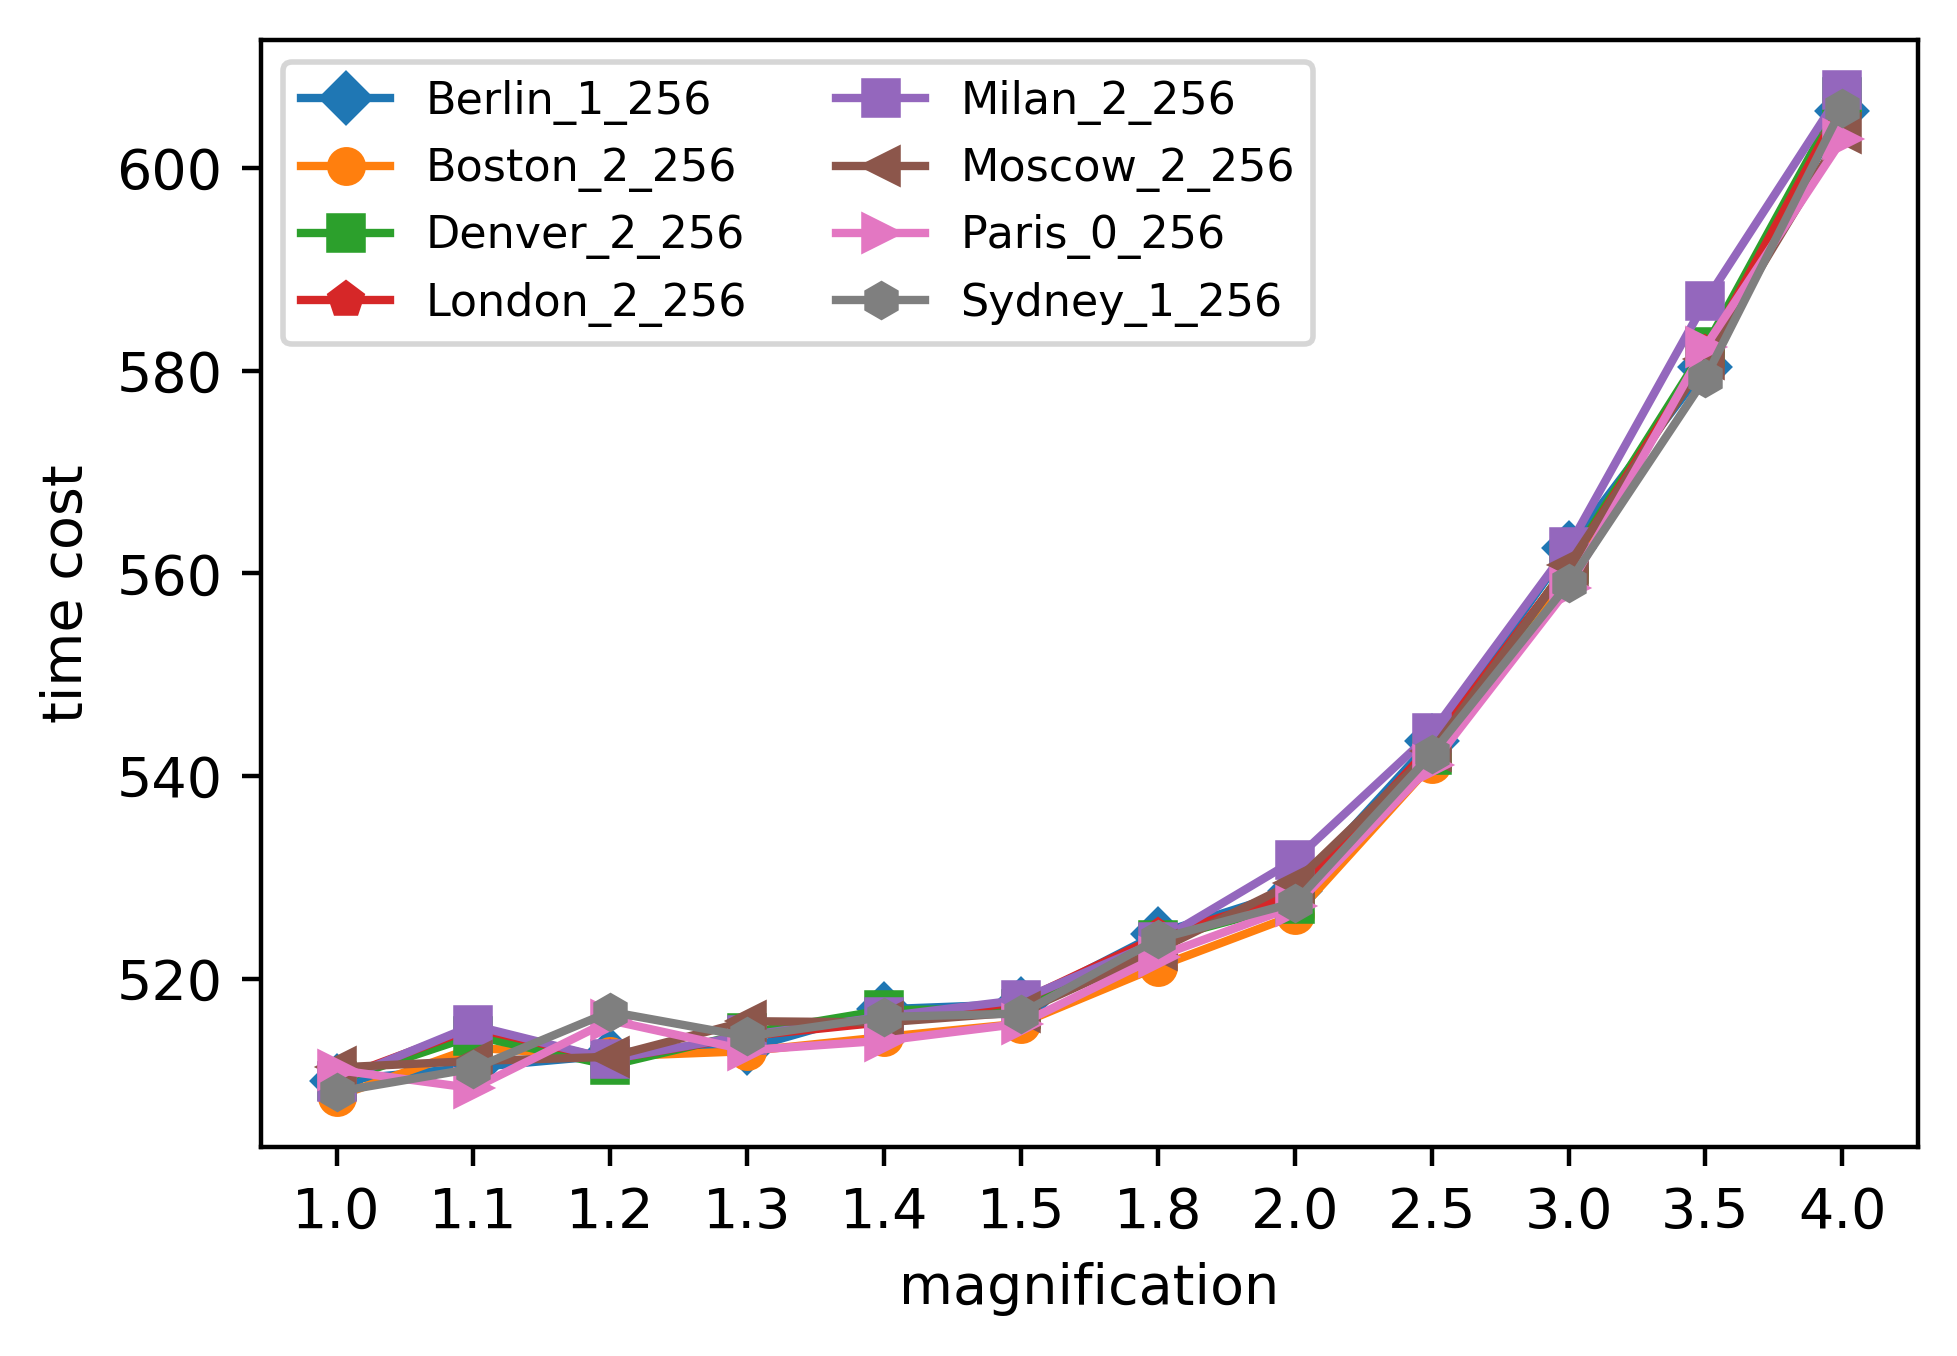
\includegraphics[width=4.6cm]{pre_time_cost.png}}
  \centerline{A: time cost comparison}
\end{minipage}
\hfill
\begin{minipage}{.48\linewidth}
  \centerline{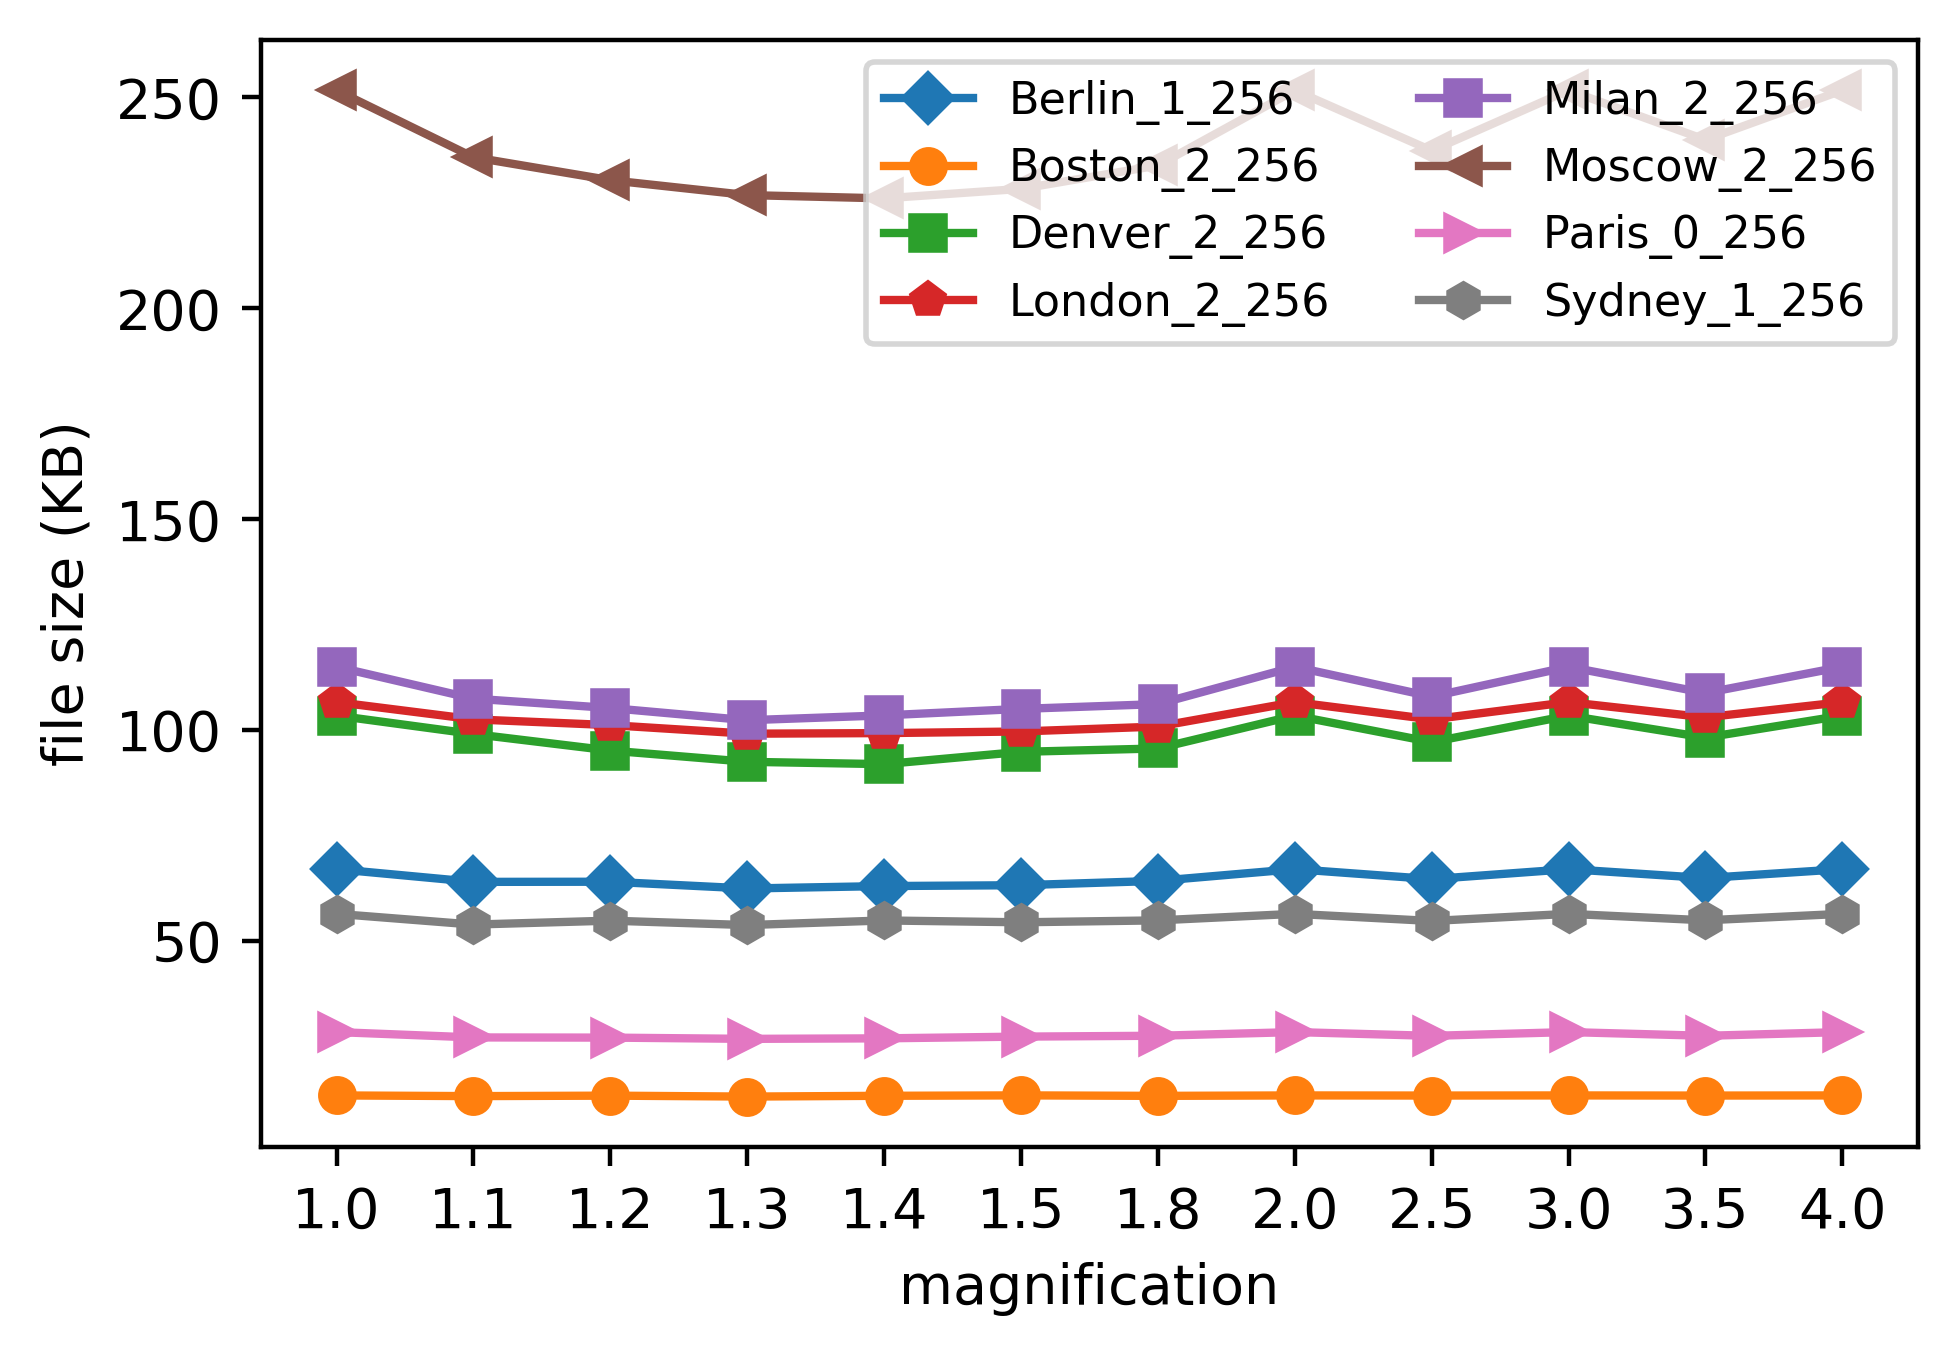
\includegraphics[width=4.6cm]{pre_file_size.png}}
  \centerline{B: time cost comparison}
\end{minipage}
\vfill

\caption{These two figures present comprehensive data pertaining to the tangent graph detection process of our method. The data includes information on time cost and file size to save the graph, encompassing various magnifications of the map. Figure 1 details the time cost across different magnifications, while Figure 2 provides insights into the corresponding file sizes.}
\label{precomputation_data}
\end{figure}

In this section, we elaborate on the construction of the tangent graph for the aforementioned eight maps across various magnifications. The associated data, including time cost and file size, is summarized in Fig \ref{precomputation_data}.

The construction of the tangent graph for nearly all maps is completed in approximately 0.5 seconds, indicating nearly real-time updates. Notably, the time cost exhibits a gradual increase as the scale magnifies. Specifically, when the map's scale increases fourfold, the time cost only experiences a 20\% increment.

The file size required to store the tangent graph for these maps ranges from 10KB to 300KB, demonstrating a manageable size for ordinary computing platforms. Importantly, the size of the tangent graph remains stable as the map scale increases. This observation suggests that the tangent graph exhibits insensitivity to variations in map resolution, making it well-suited for real-world maps with high resolutions.


\subsection{Comparison with other methods}
%In this section, we focus on compare our method with other methods, including HA*, HTheta* and RHCF. In practice, distinctive topology path planning have a time cost upper bound, to avoid cost more time than expectation. And if a method finds no all solution within the time bound, it return all solution it have found. So in section, we set the time upper bound to 10s, and apply the success rate to find all solution within time bound as a indicator to evaluate the performance of methods. Essentially, success rate is determine by time cost.

%Moreover, we compare all methods in terms of path length, which is also a very important indicator in path planning. Considering map scale have a siginicant influence on the performance path planning algorithms, we also test the four mentioned methods under map have the same content but scale range from 256*256 to 1024*1024.
    
In this section, our focus centers on the comparative analysis of our method with other prominent approaches, namely HA*, HTheta*, and RHCF. In practical applications, topologically distinctive path planning is often constrained by an upper limit on time costs to avoid exceeding expected time constraints. When a method fails to find all solutions within the specified time bound, it returns the solutions it has discovered up to that point. Therefore, in this section, we impose a time upper bound of 10 seconds and employ the success rate – the ability to find all solutions within the time constraint – as an indicative measure for evaluating the performance of the methods. Essentially, the success rate is determined by the time cost incurred.

Furthermore, we conduct a comparative assessment of all methods with respect to path length – a crucial metric in path planning. Recognizing that map scale significantly influences the performance of path planning algorithms, we conduct tests on the four aforementioned methods using maps with identical content but scales ranging from 256$\times$256 to 1024$\times$1024.    
    
\subsubsection{Time cost and success rate}

% total time cost and required path count
\begin{figure*}[t] \scriptsize
%\begin{tabular}{cc}
\begin{minipage}{.245\linewidth}
  \centerline{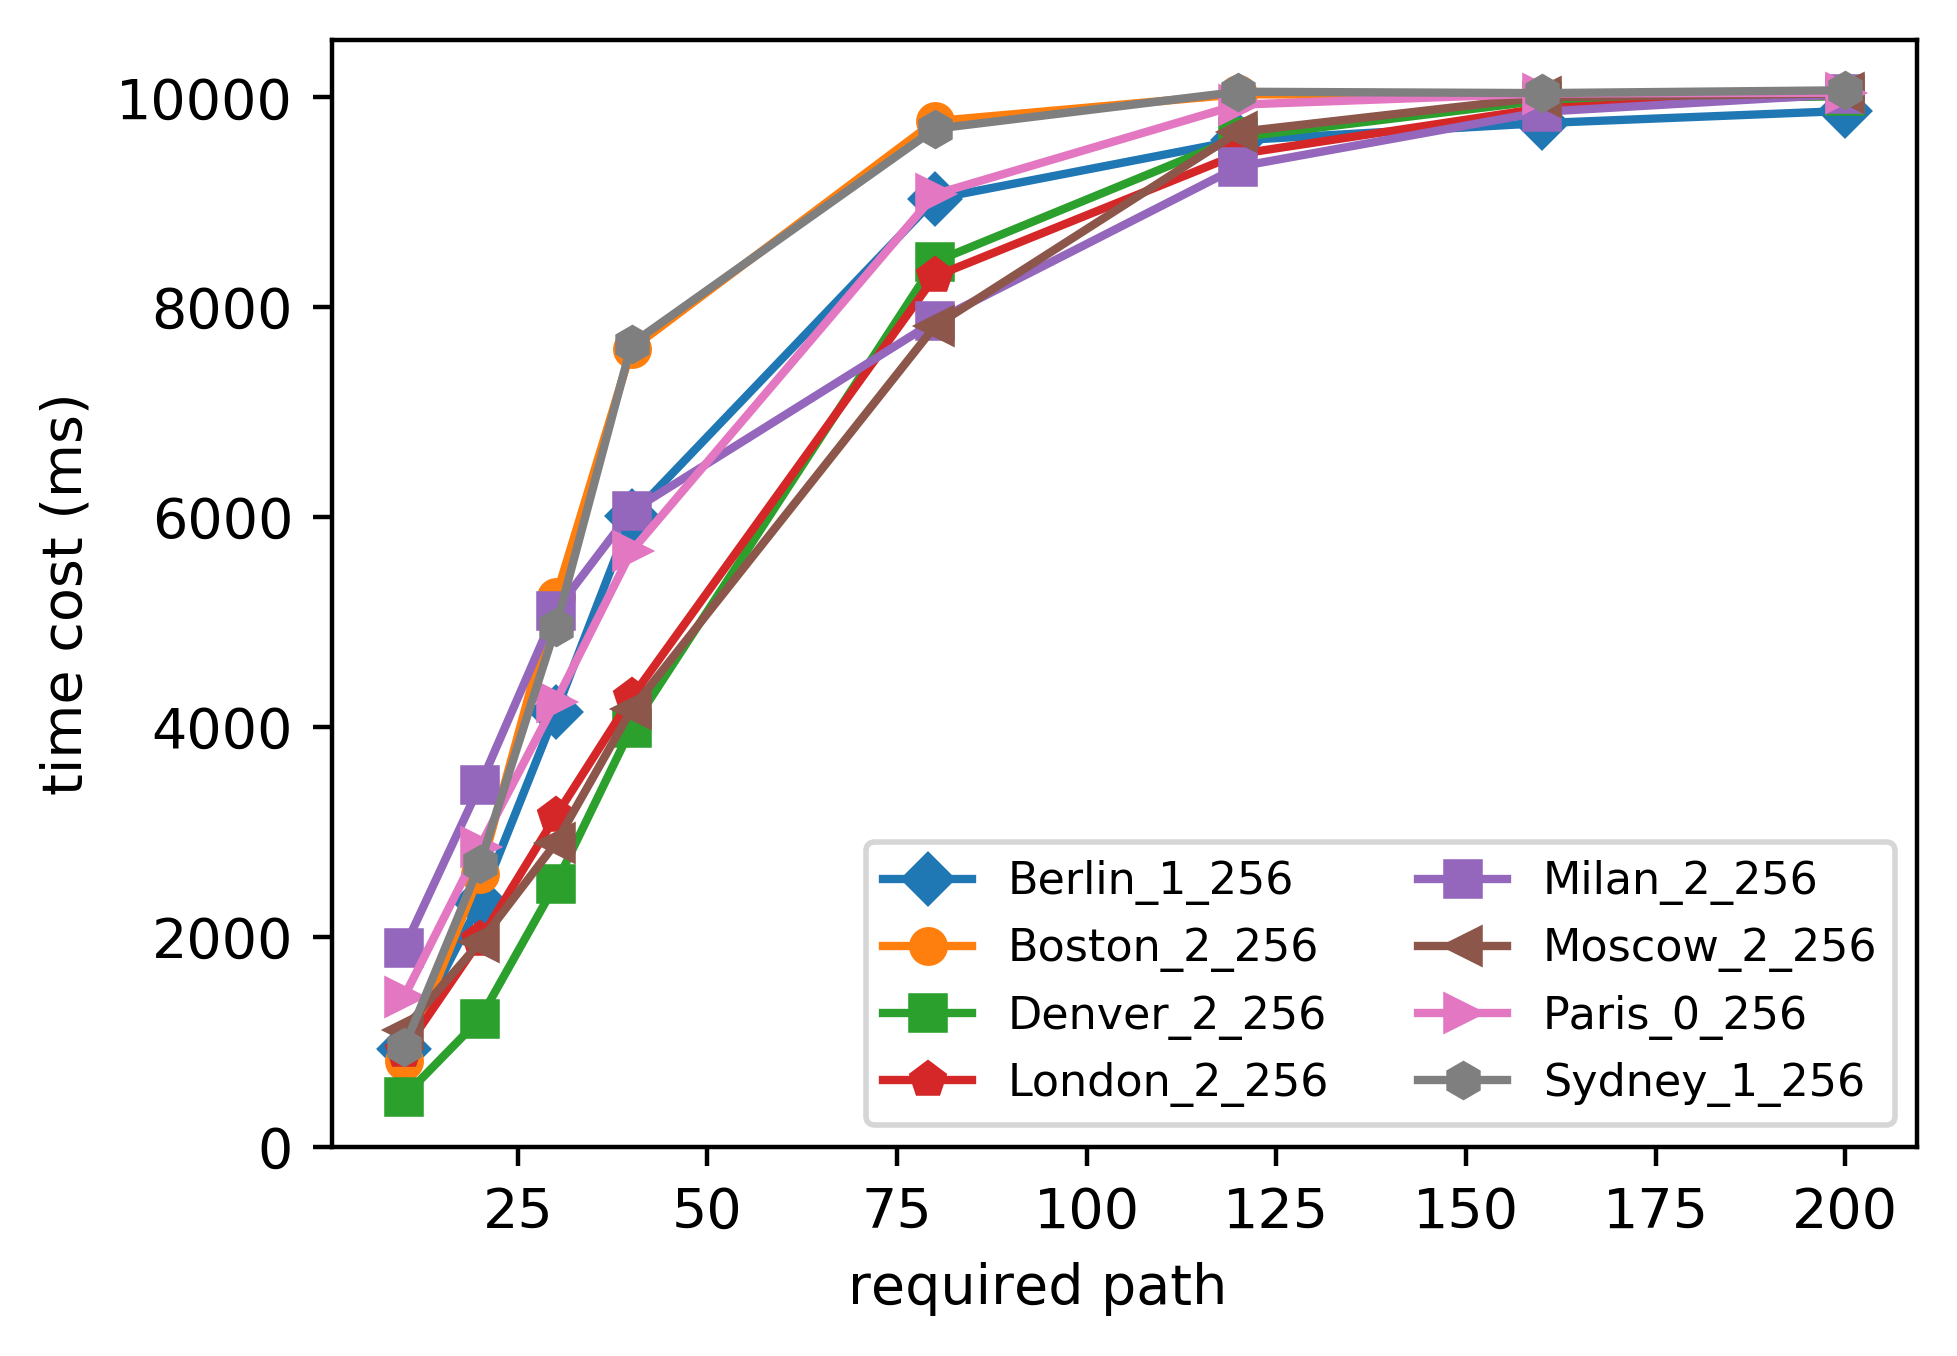
\includegraphics[width=4.6cm]{HsAs_time_and_count.png}}
  \centerline{A: HA*}
\end{minipage}
\hfill
\begin{minipage}{.245\linewidth}
  \centerline{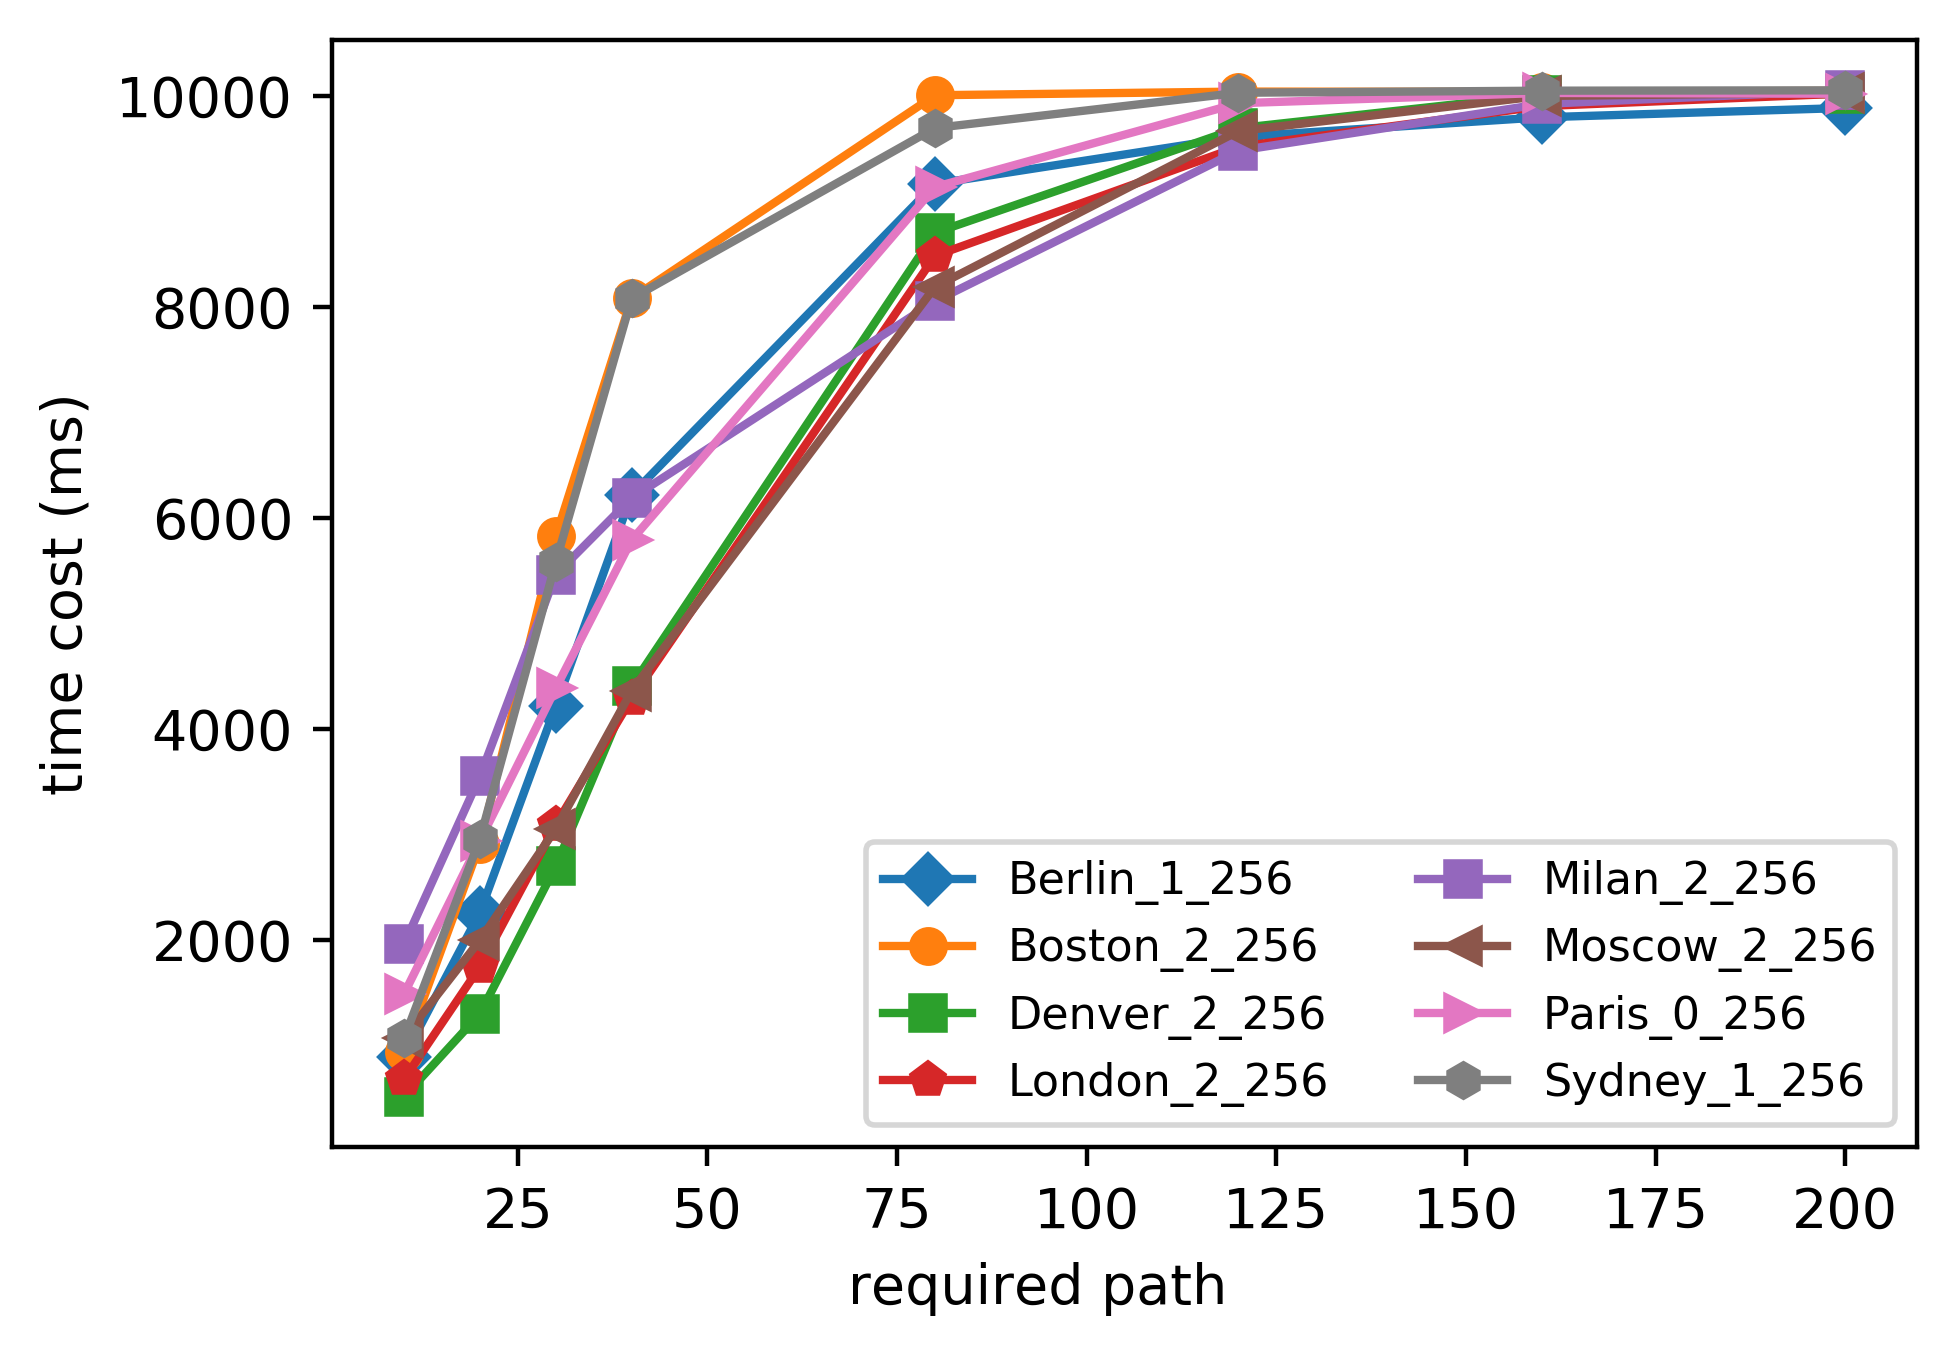
\includegraphics[width=4.6cm]{HsTs_time_and_count.png}}
  \centerline{B: HTheta*}
\end{minipage}
\hfill
\begin{minipage}{.245\linewidth}
  \centerline{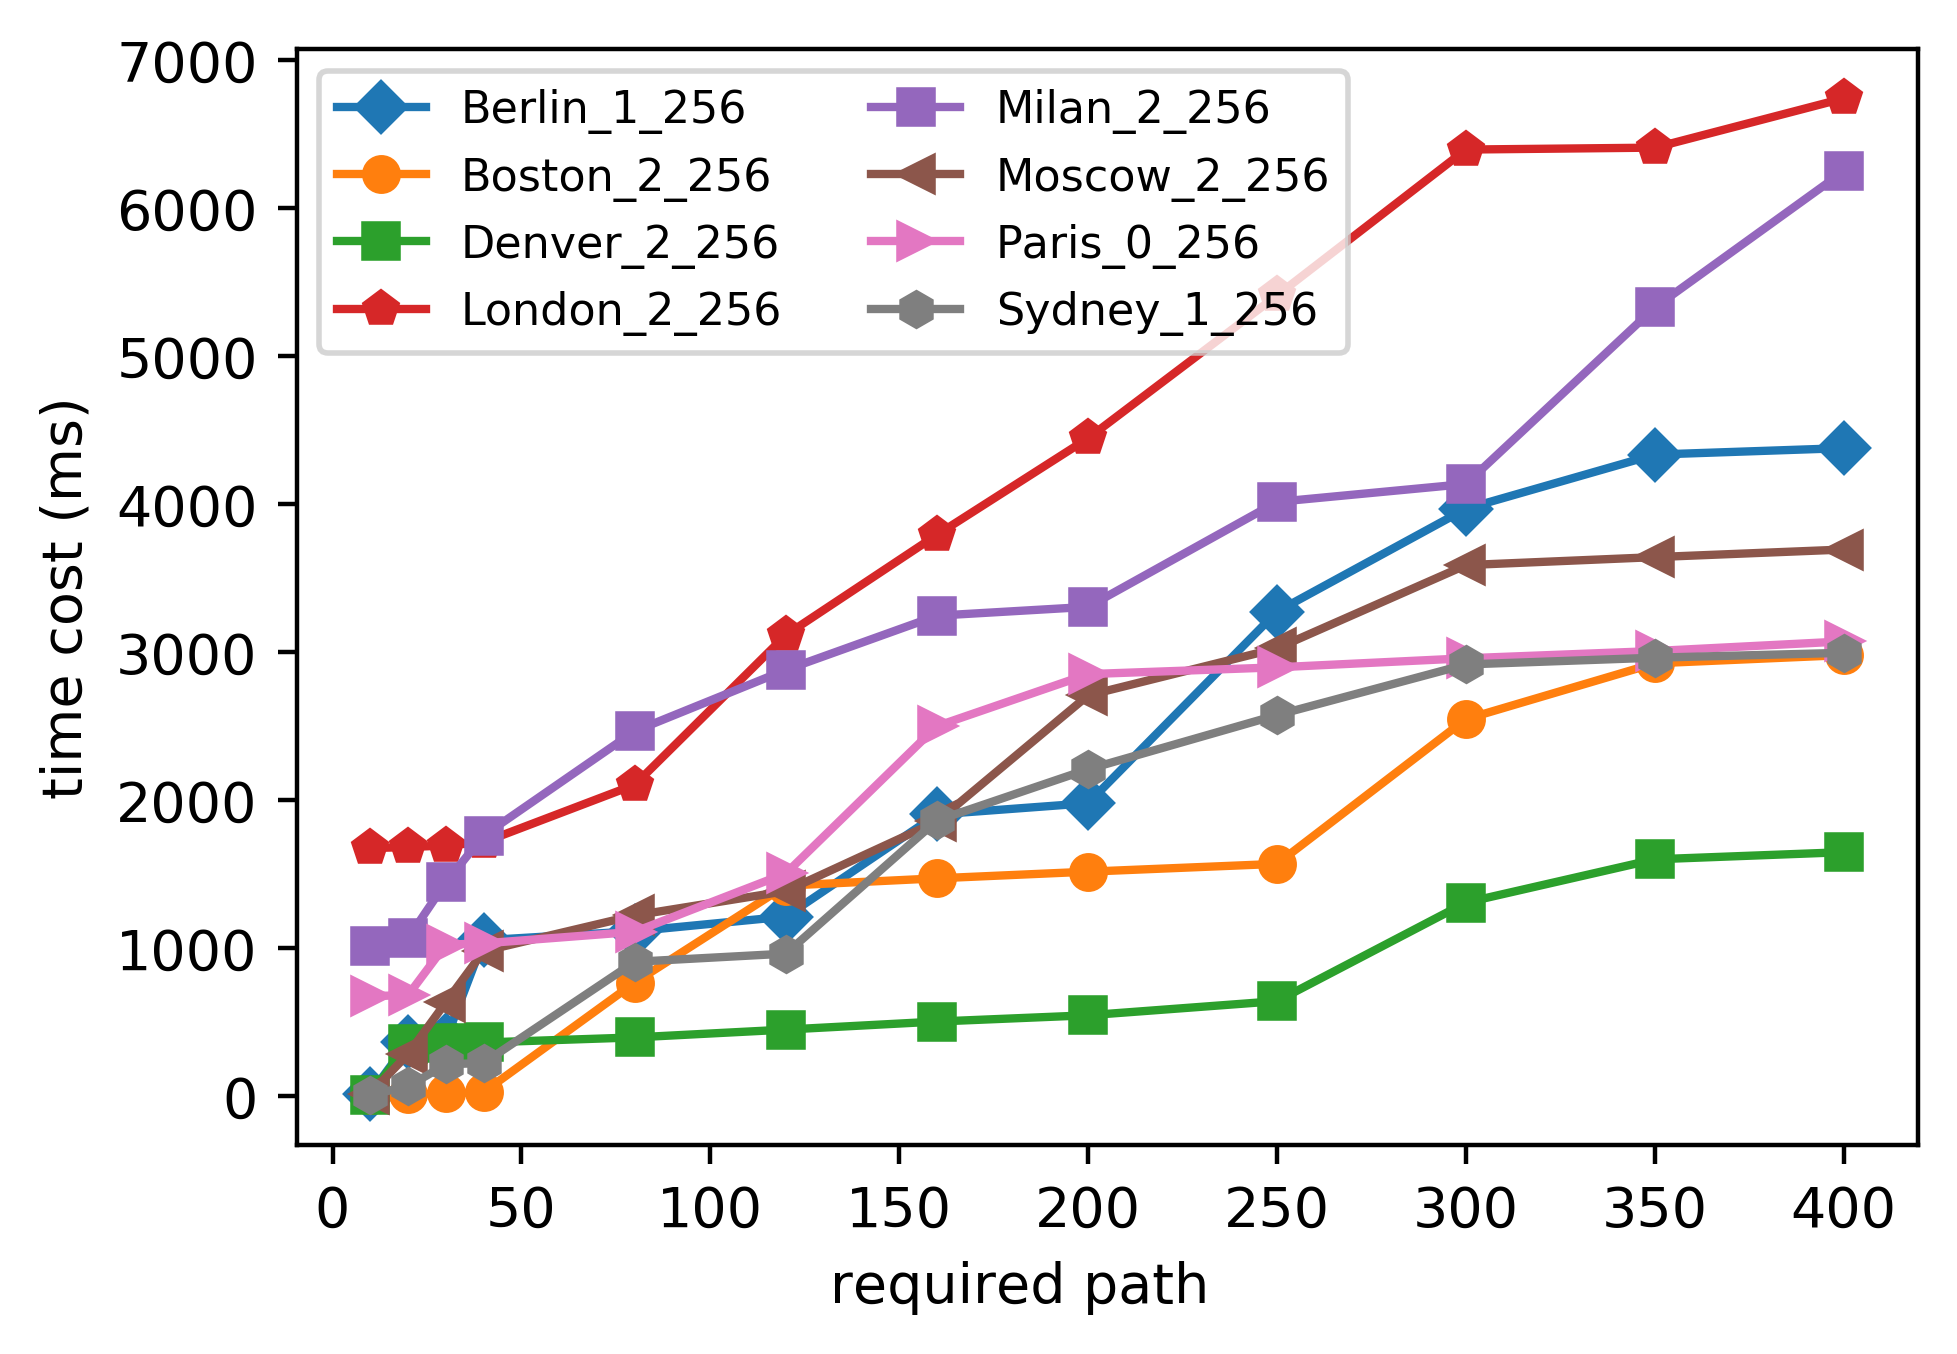
\includegraphics[width=4.6cm]{RHCF_time_and_count.png}}
  \centerline{C: RHCF}
\end{minipage}
\hfill
\begin{minipage}{.245\linewidth}
  \centerline{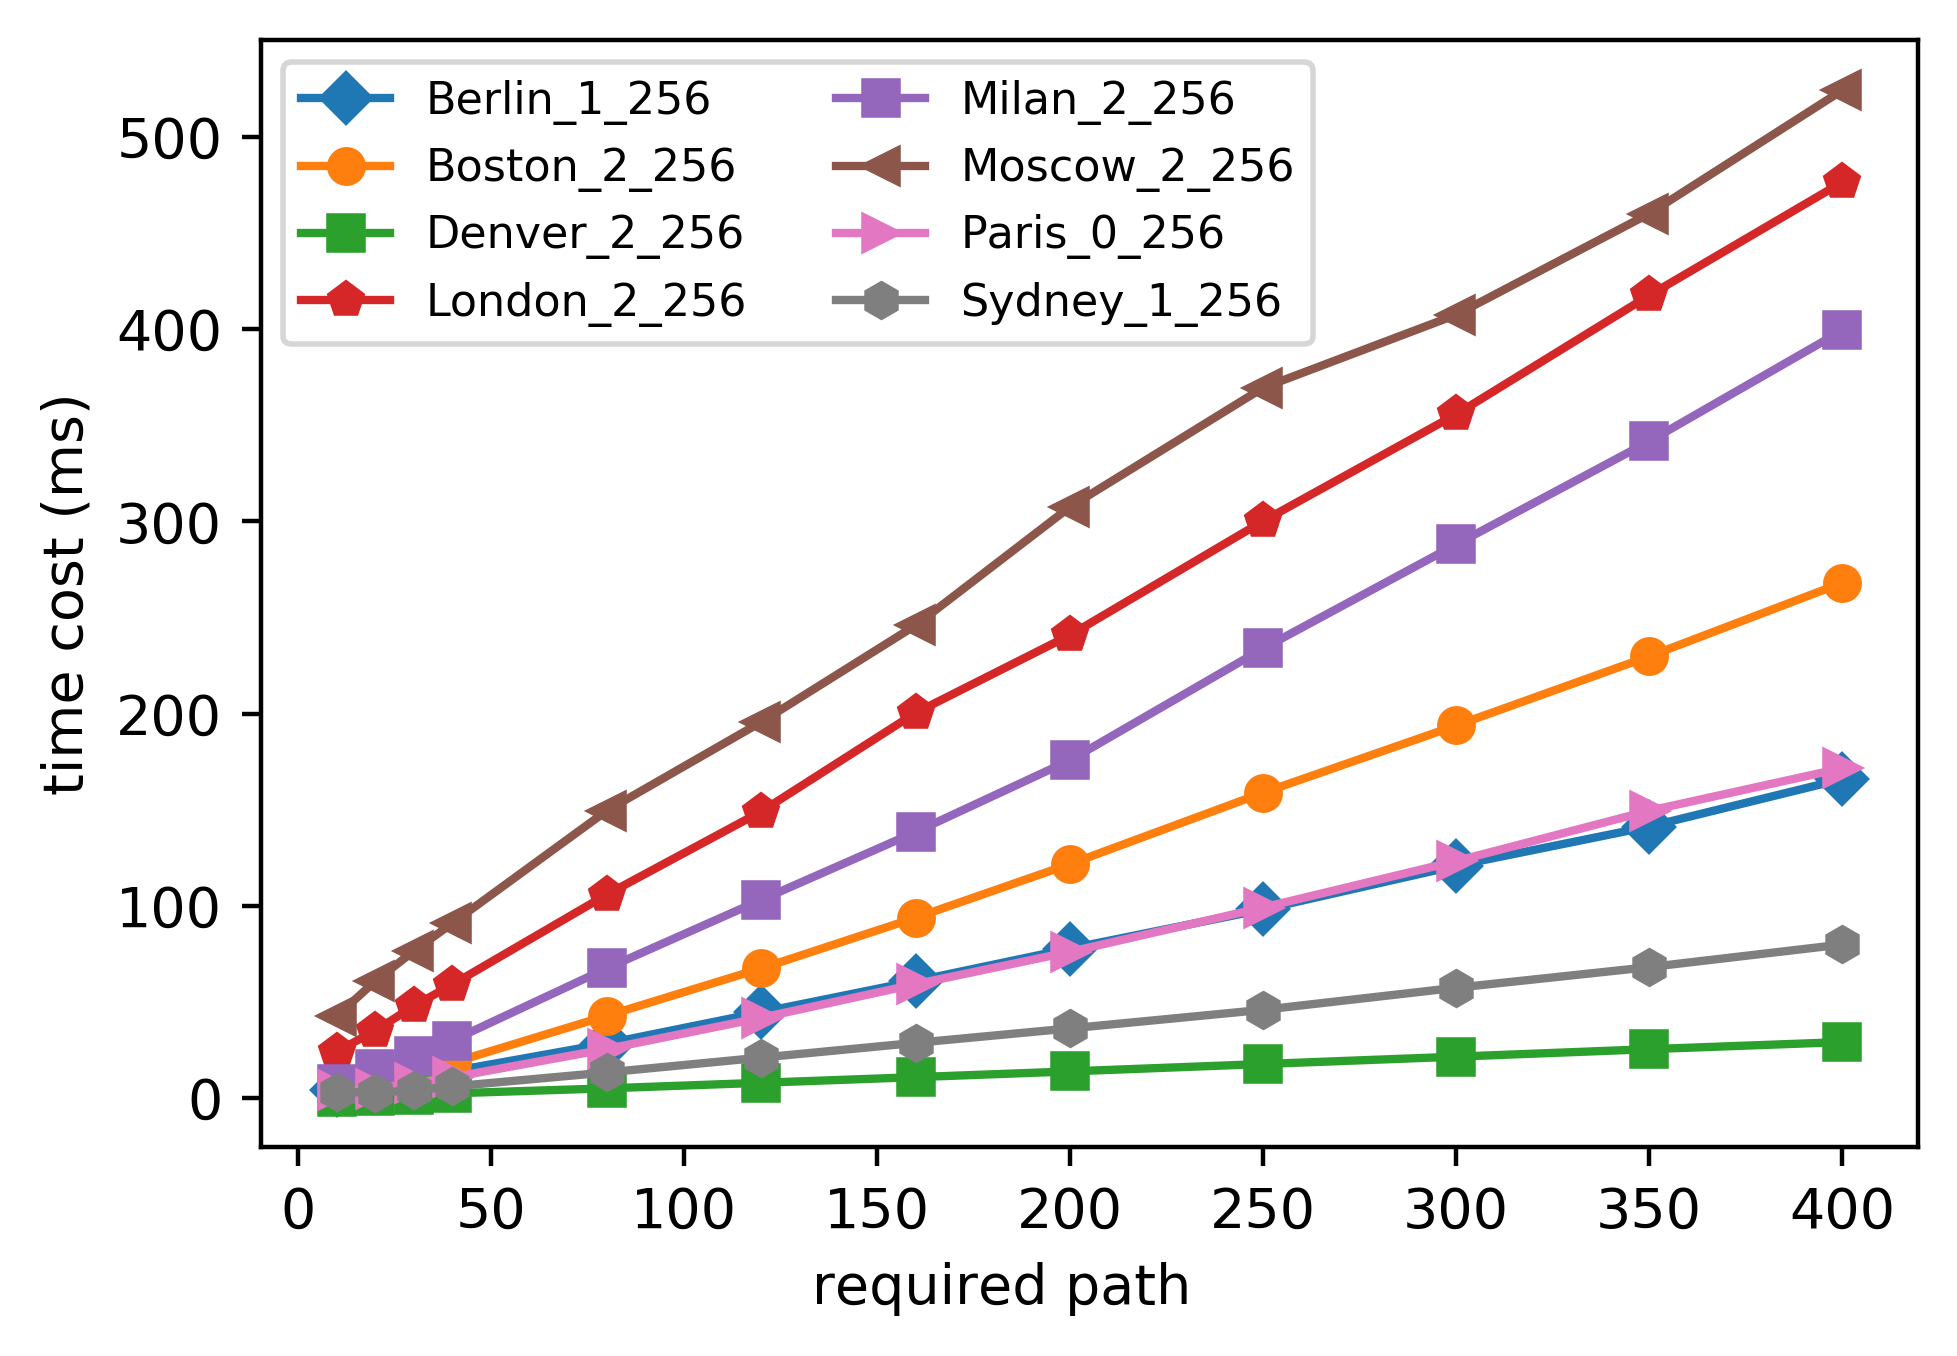
\includegraphics[width=4.6cm]{RJ_time_and_count.png}}
  \centerline{D: Our method}
\end{minipage}
\vfill

\caption{These figures illustrate the mean time cost for finding the required number of paths for each map using all four methods. The magnification for all maps is set to 1.0.}
\label{total_time_cost_and_path_count}
\end{figure*}

% success rate and required path count
\begin{figure*}[t] \scriptsize
%\begin{tabular}{cc}
\begin{minipage}{.245\linewidth}
  \centerline{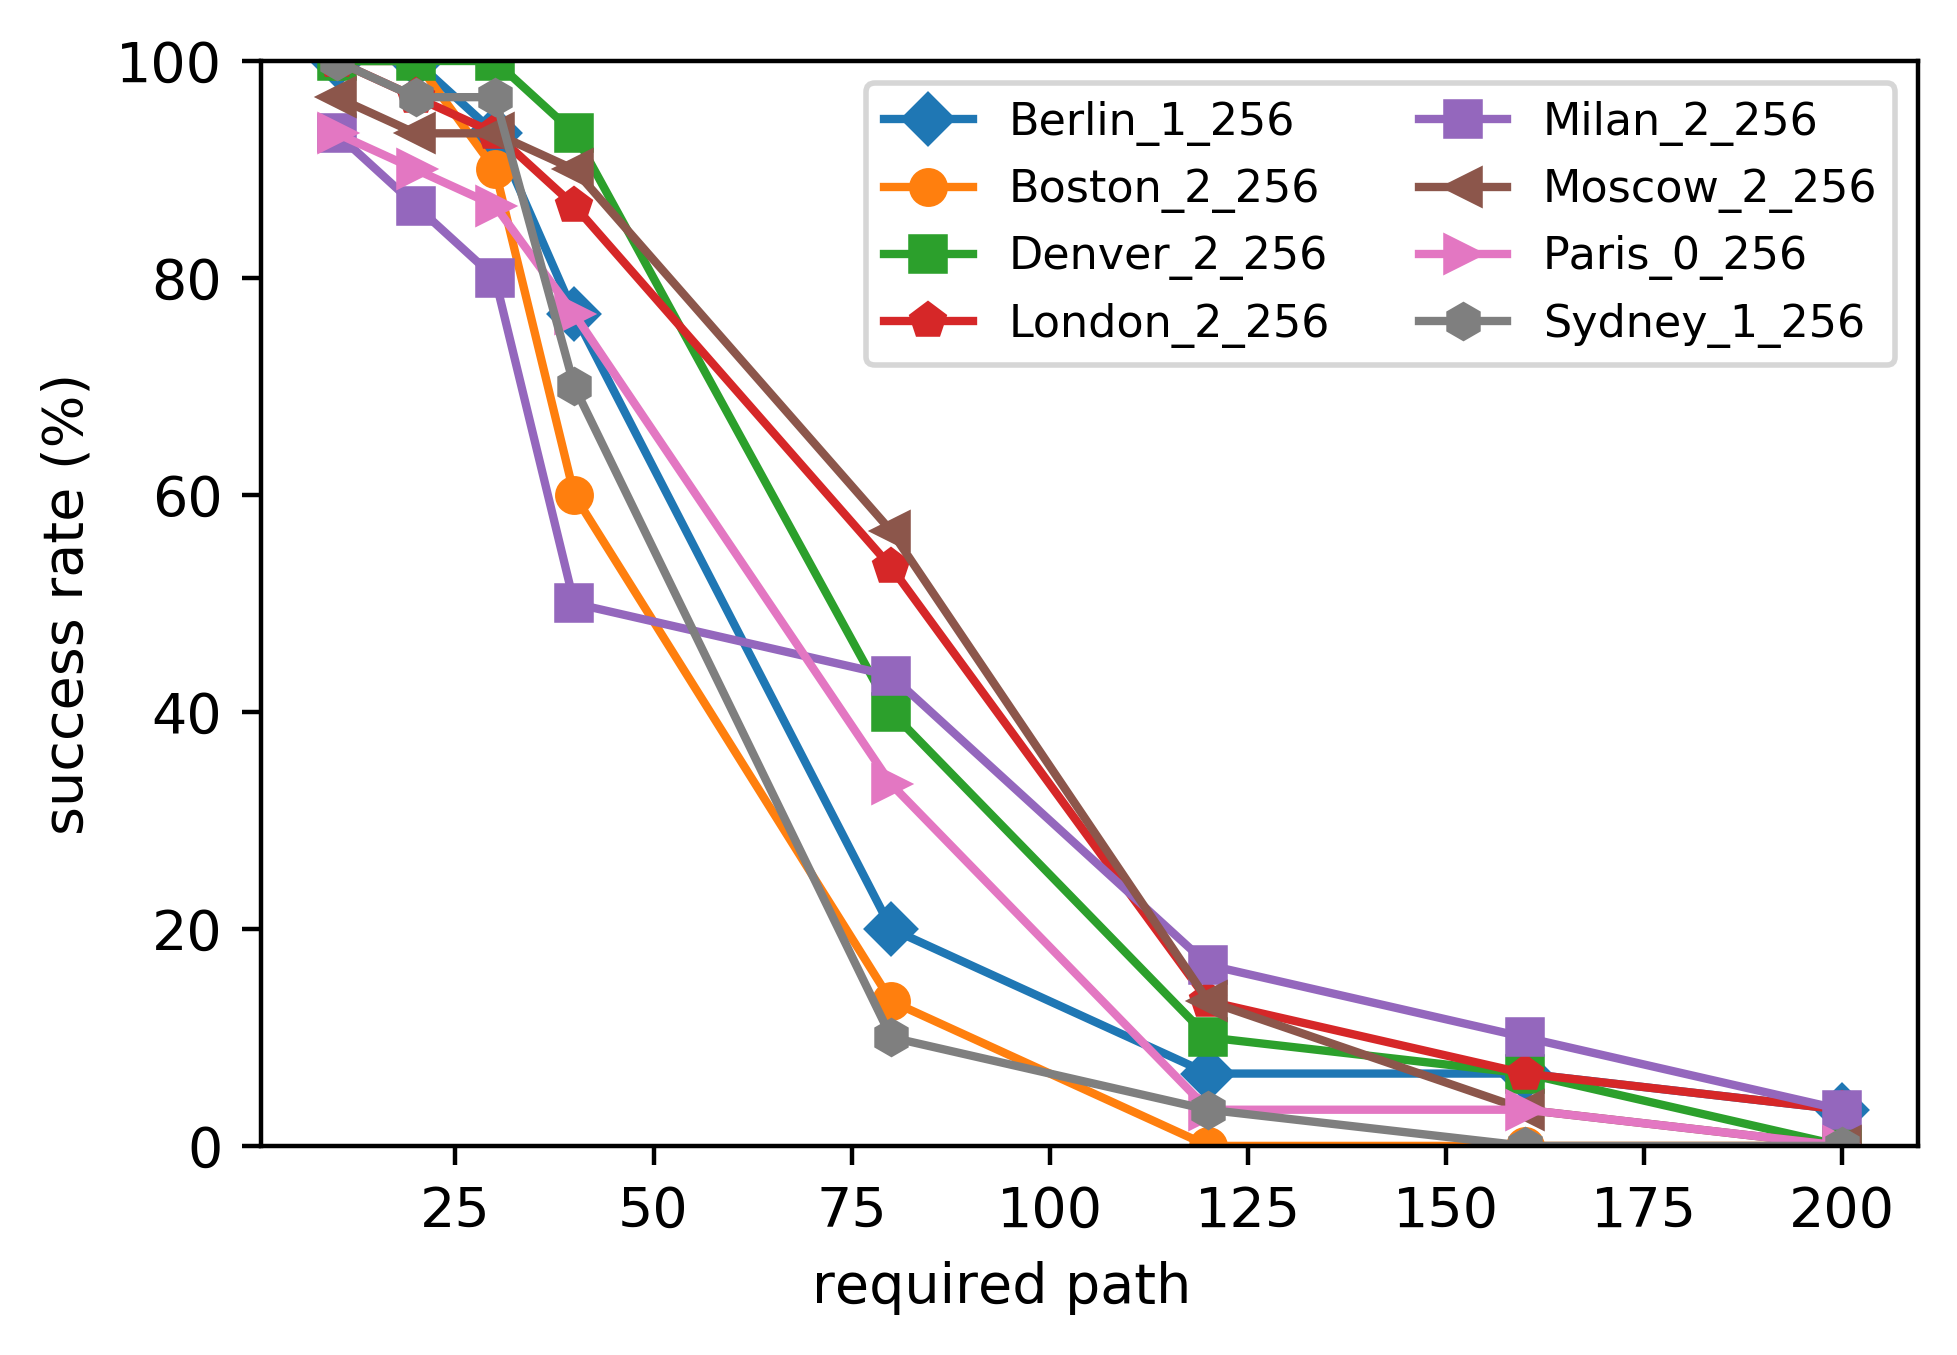
\includegraphics[width=4.6cm]{HsAs_succ_and_count.png}}
  \centerline{A: HA*}
\end{minipage}
\hfill
\begin{minipage}{.245\linewidth}
  \centerline{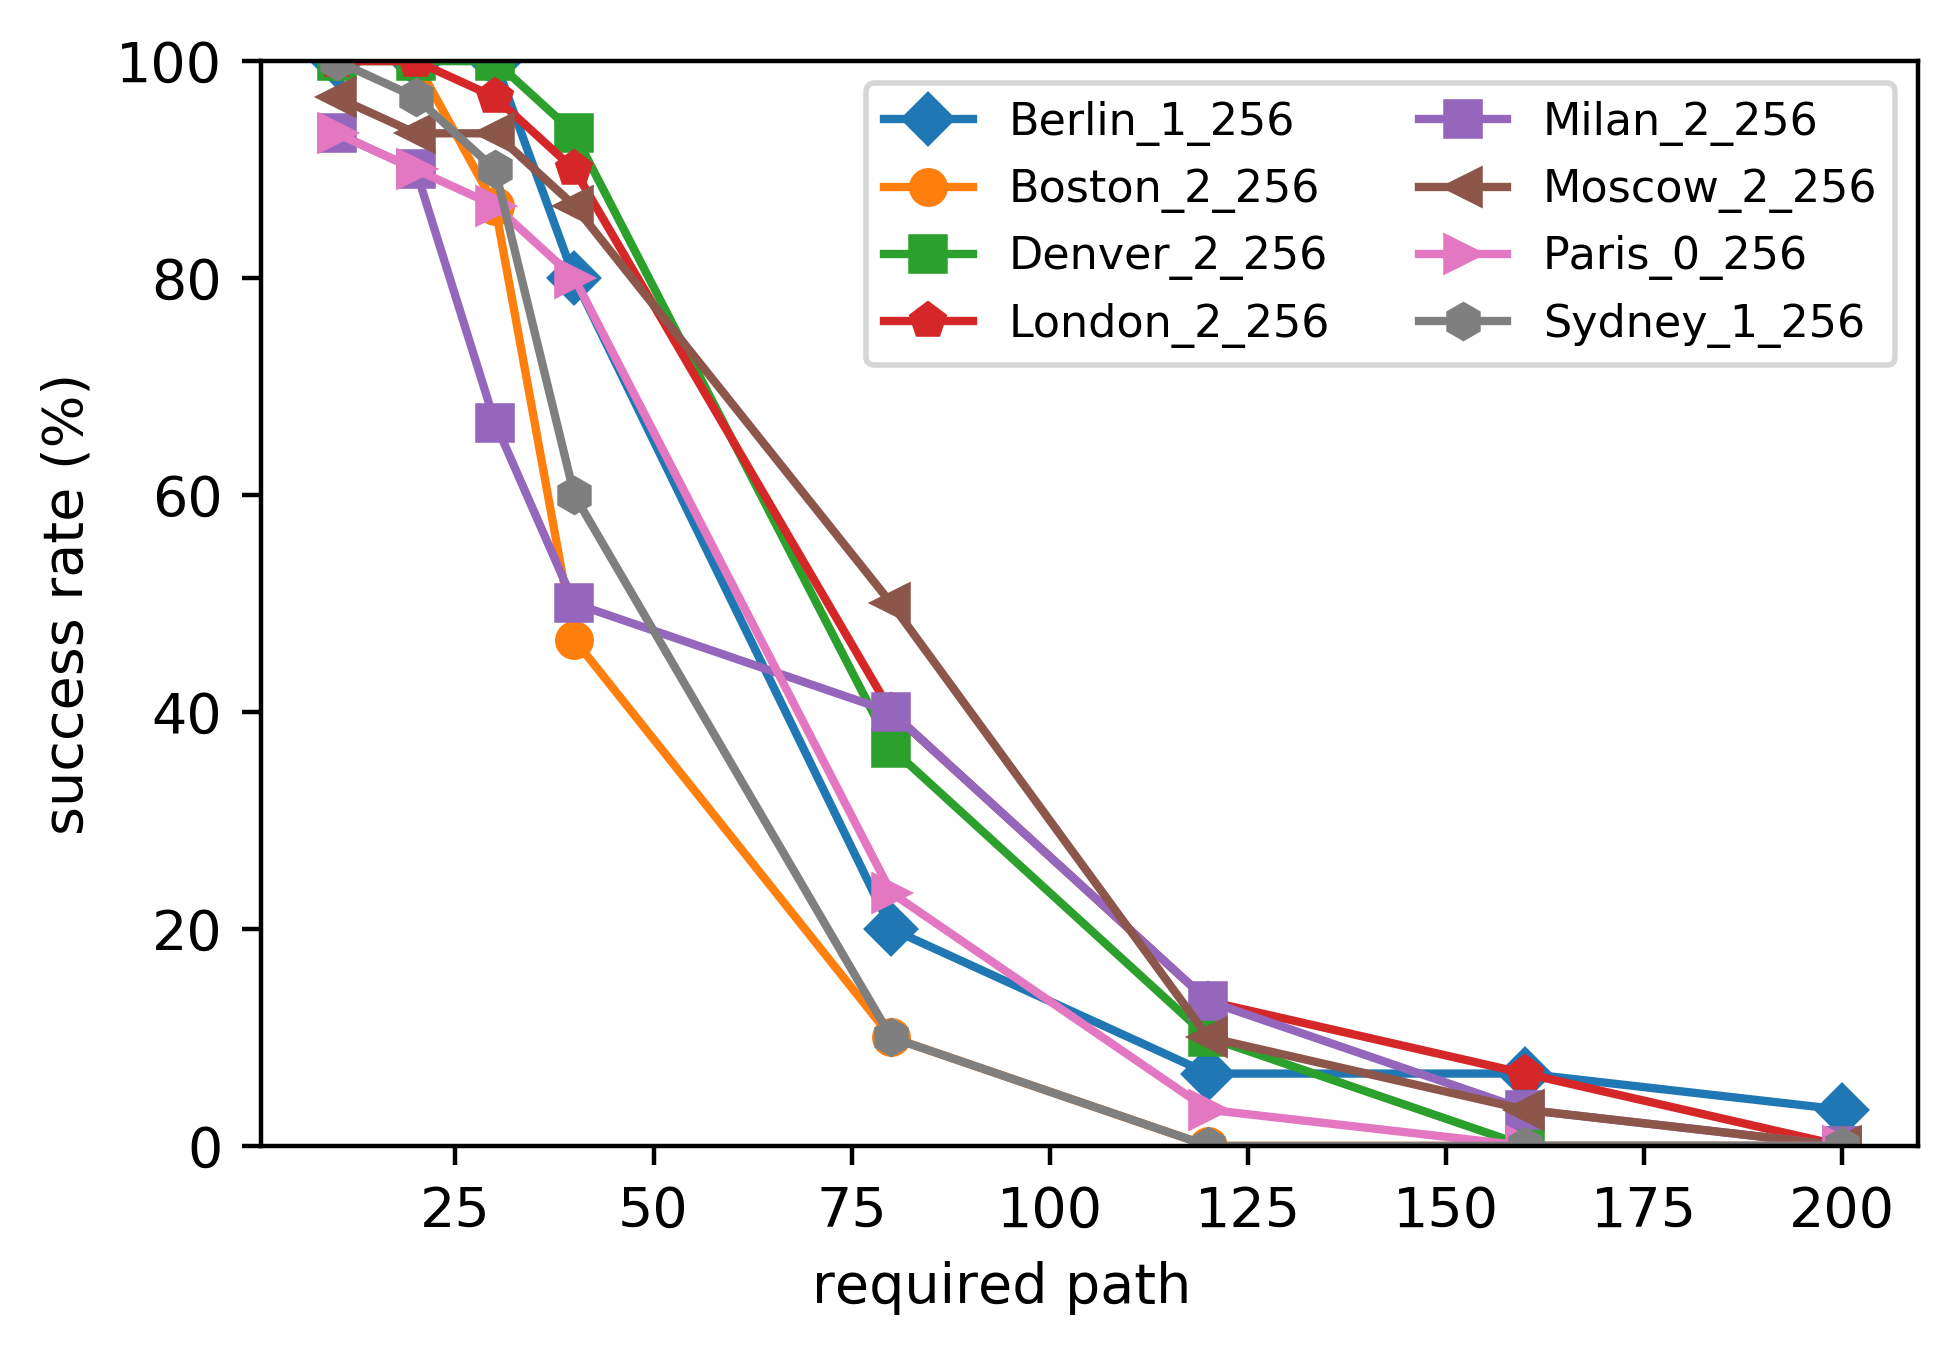
\includegraphics[width=4.6cm]{HsTs_succ_and_count.png}}
  \centerline{B: HTheta*}
\end{minipage}
\hfill
\begin{minipage}{.245\linewidth}
  \centerline{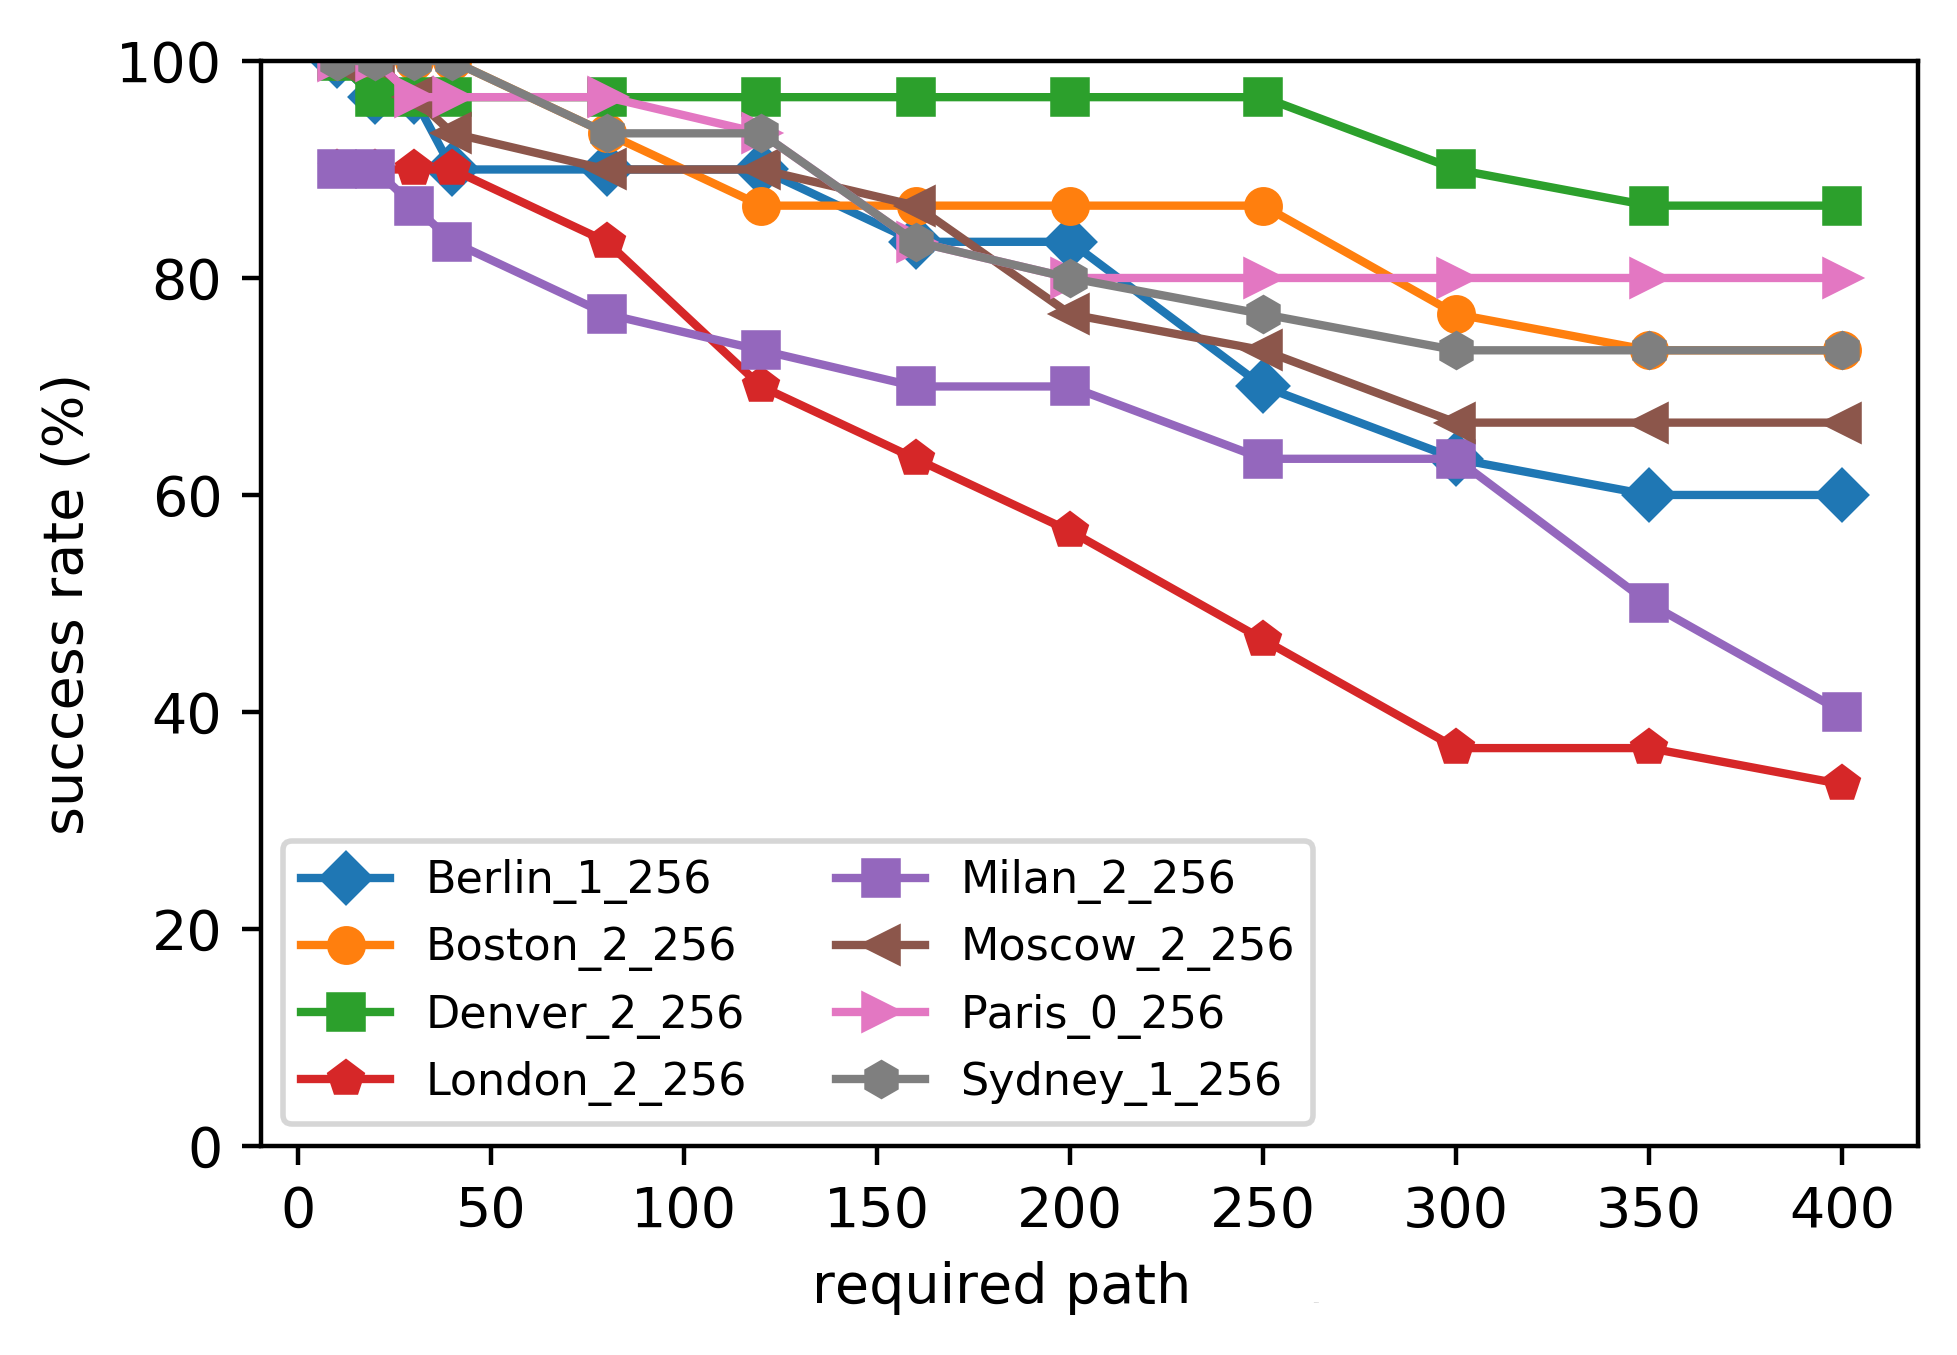
\includegraphics[width=4.6cm]{RHCF_succ_and_count.png}}
  \centerline{C: RHCF}
\end{minipage}
\hfill
\begin{minipage}{.245\linewidth}
  \centerline{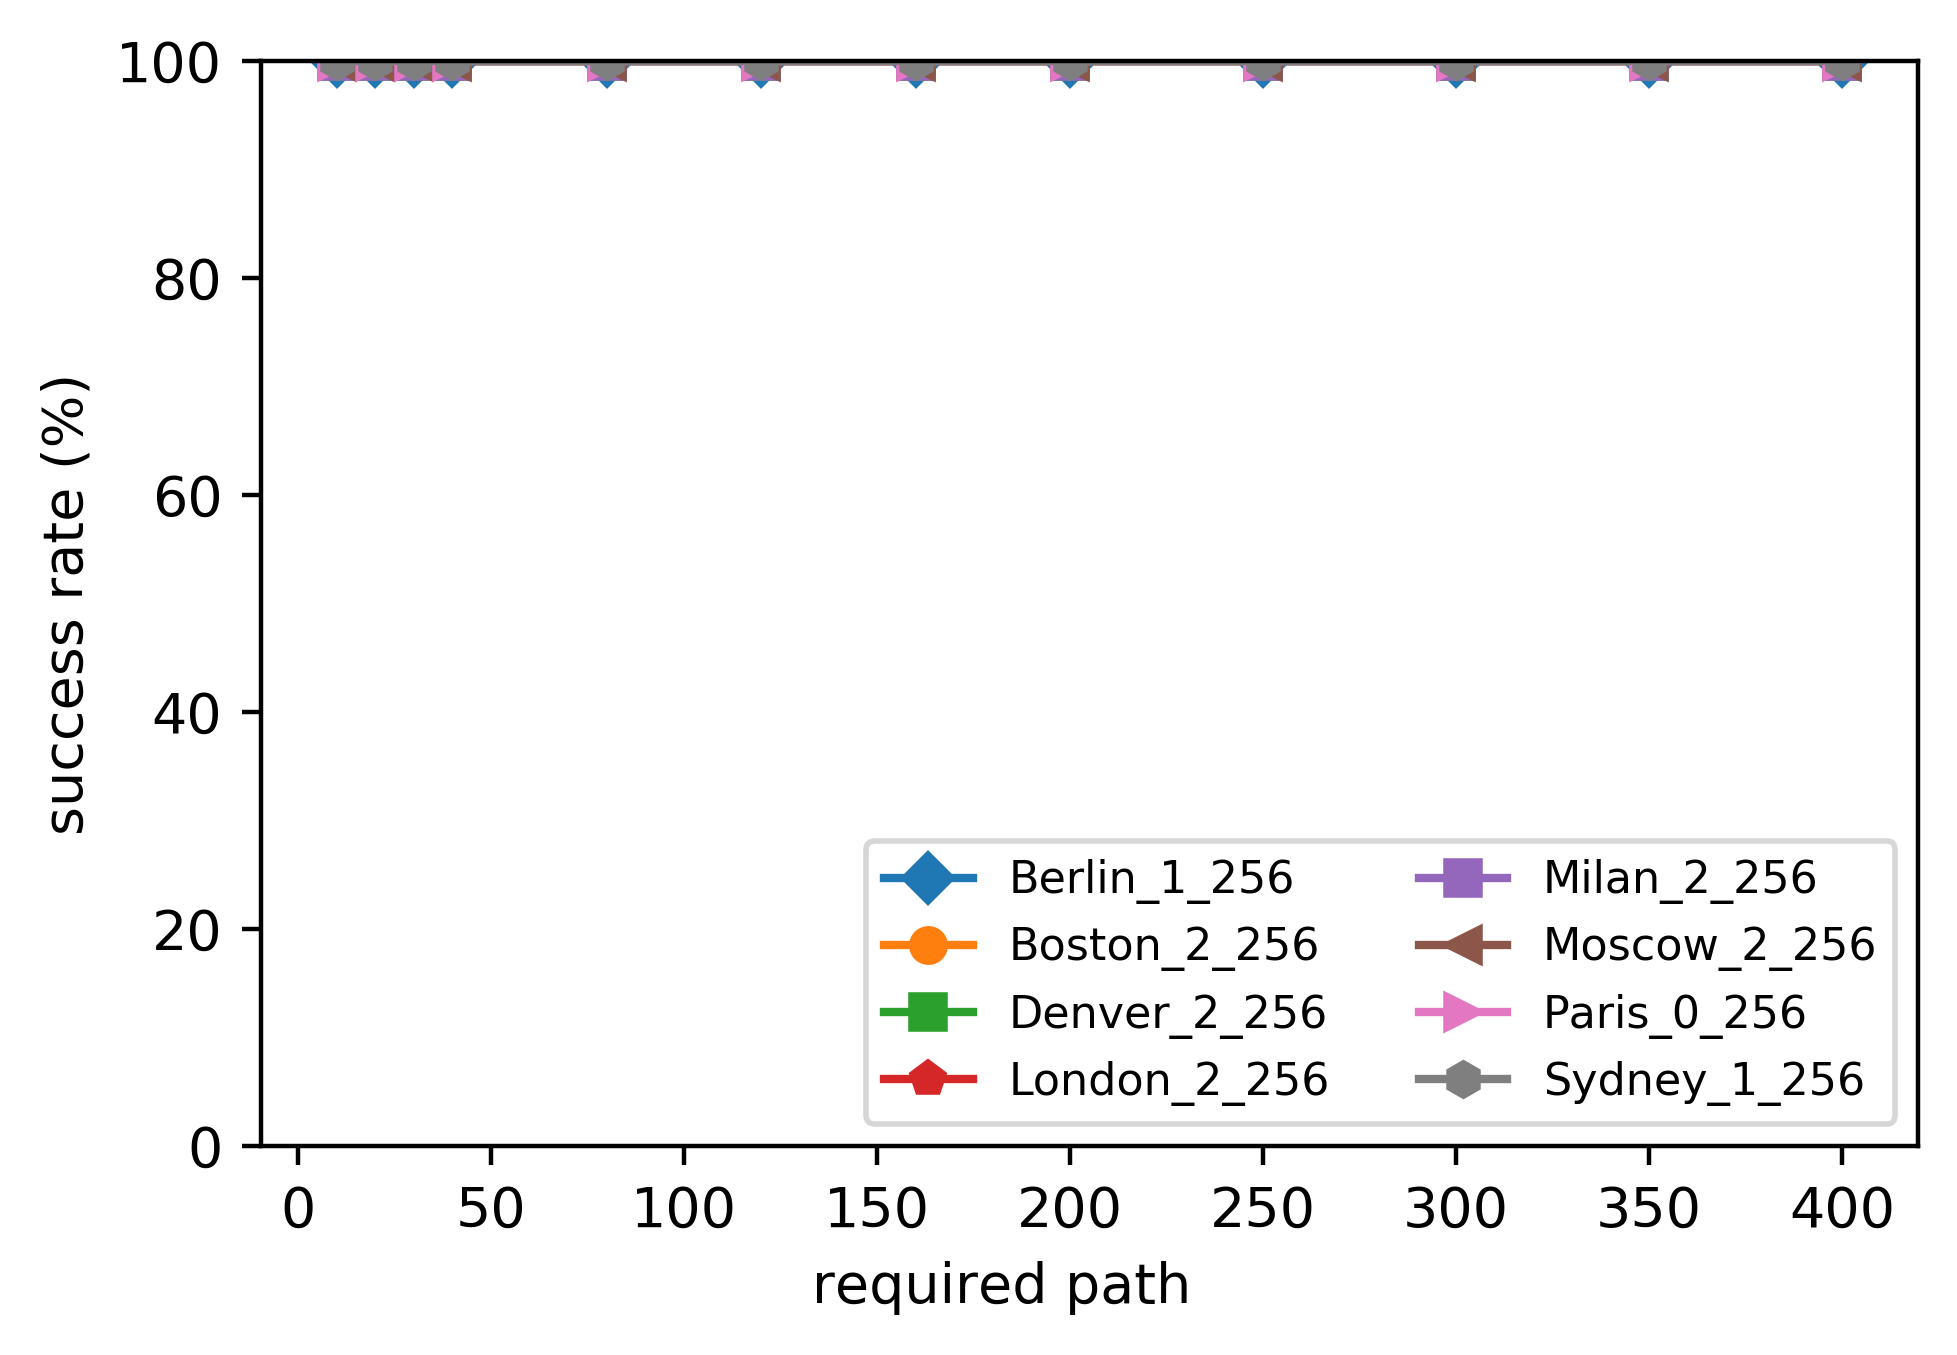
\includegraphics[width=4.6cm]{RJ_succ_and_count.png}}
  \centerline{D: Our method}
\end{minipage}
\vfill

\caption{These figures illustrate the mean success rate for finding the required number of paths for each map using all four methods. The magnification for all maps is set to 1.0. 
}
\label{succ_and_path_count}
\end{figure*}

\begin{figure}[t] \scriptsize
%\begin{tabular}{cc}
\begin{minipage}{.48\linewidth}
  \centerline{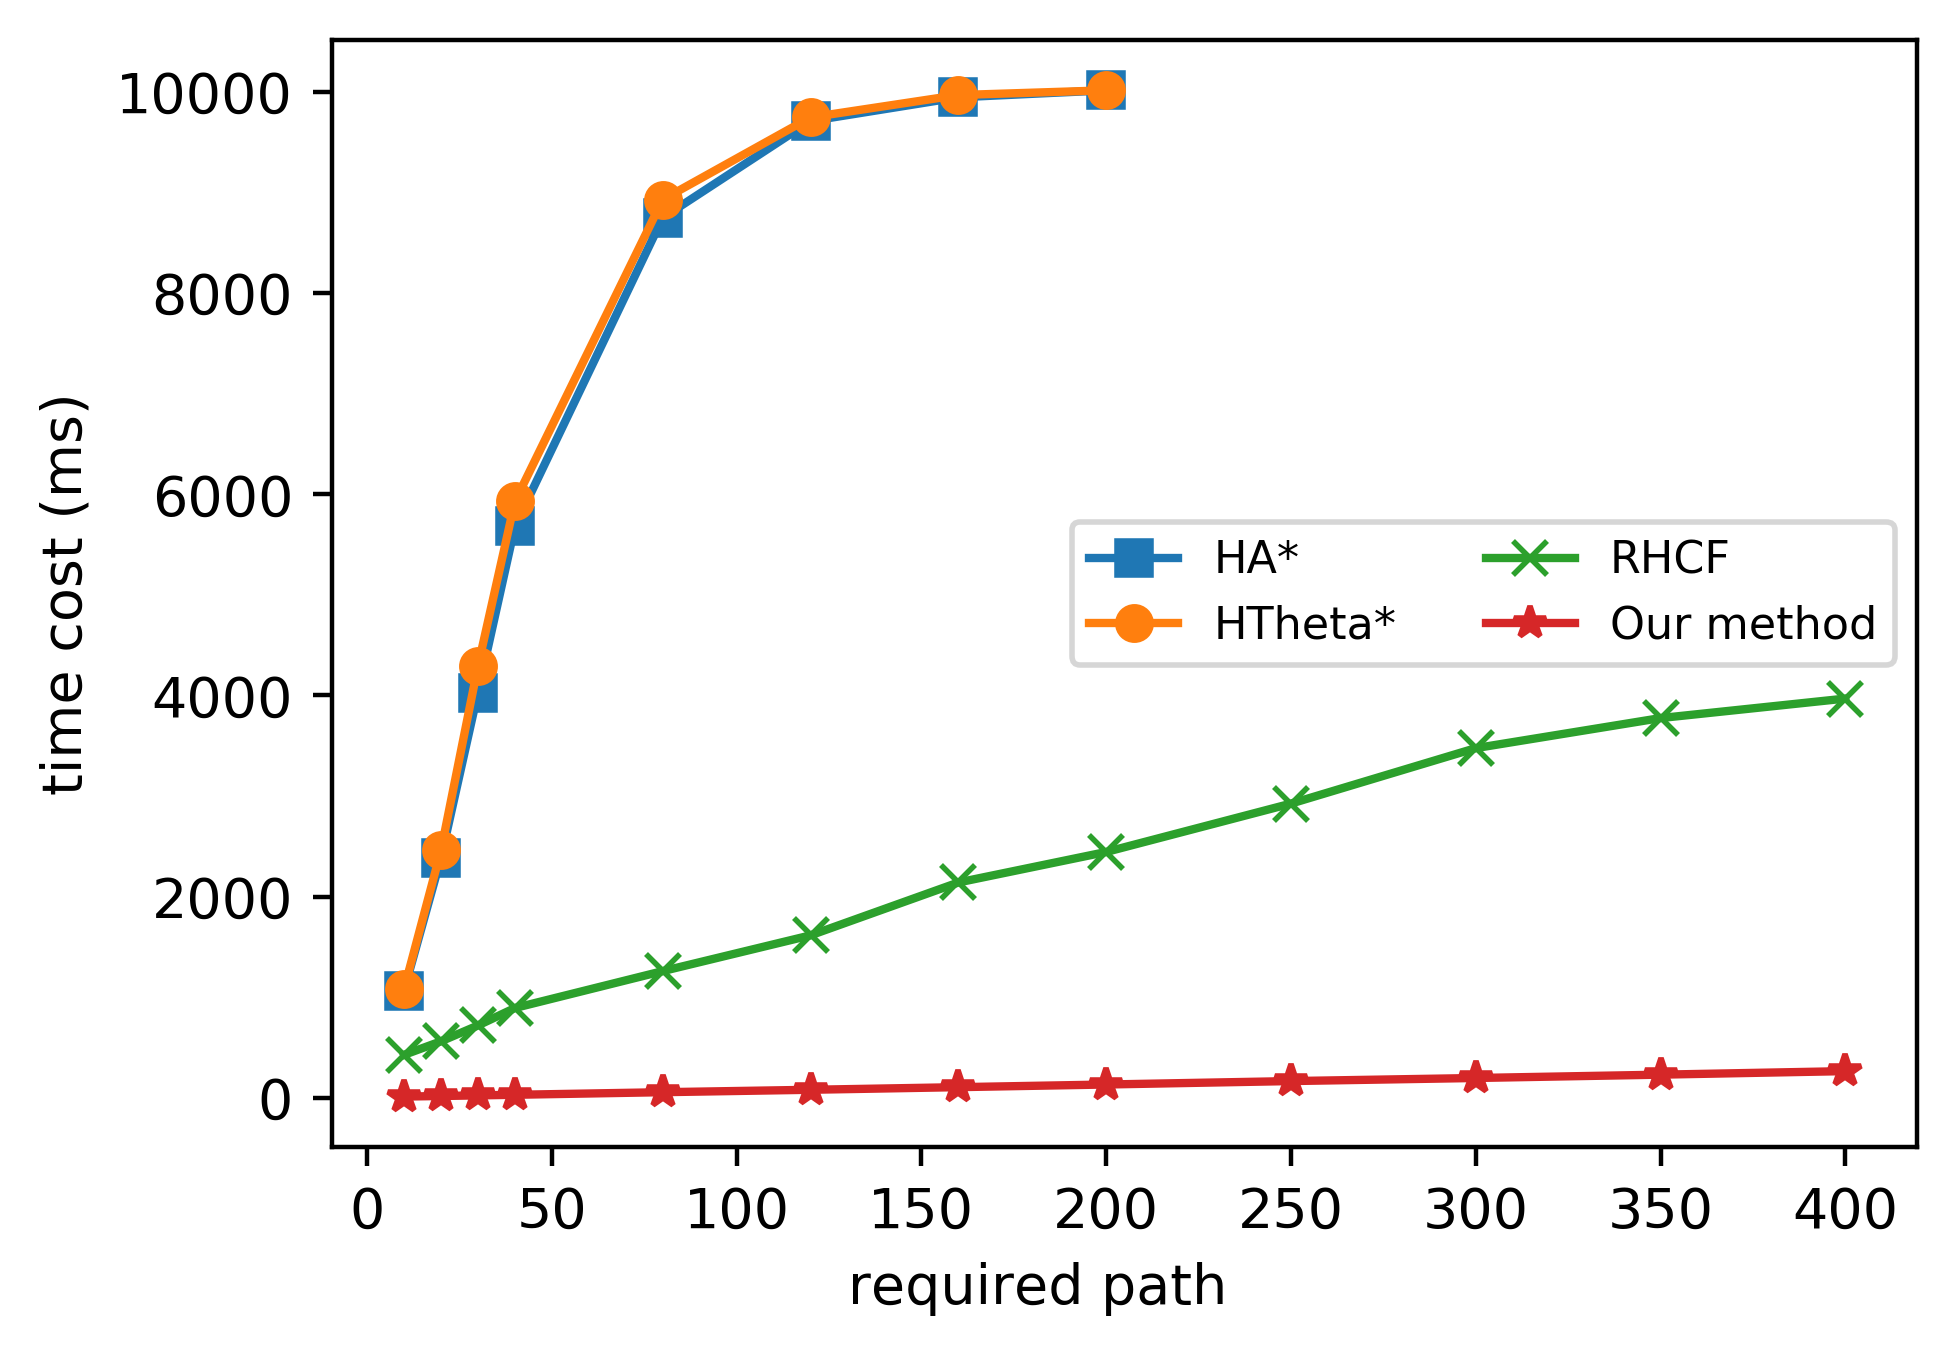
\includegraphics[width=4.6cm]{comparison_time_and_count.png}}
  \centerline{A: time cost comparison}
\end{minipage}
\hfill
\begin{minipage}{.48\linewidth}
  \centerline{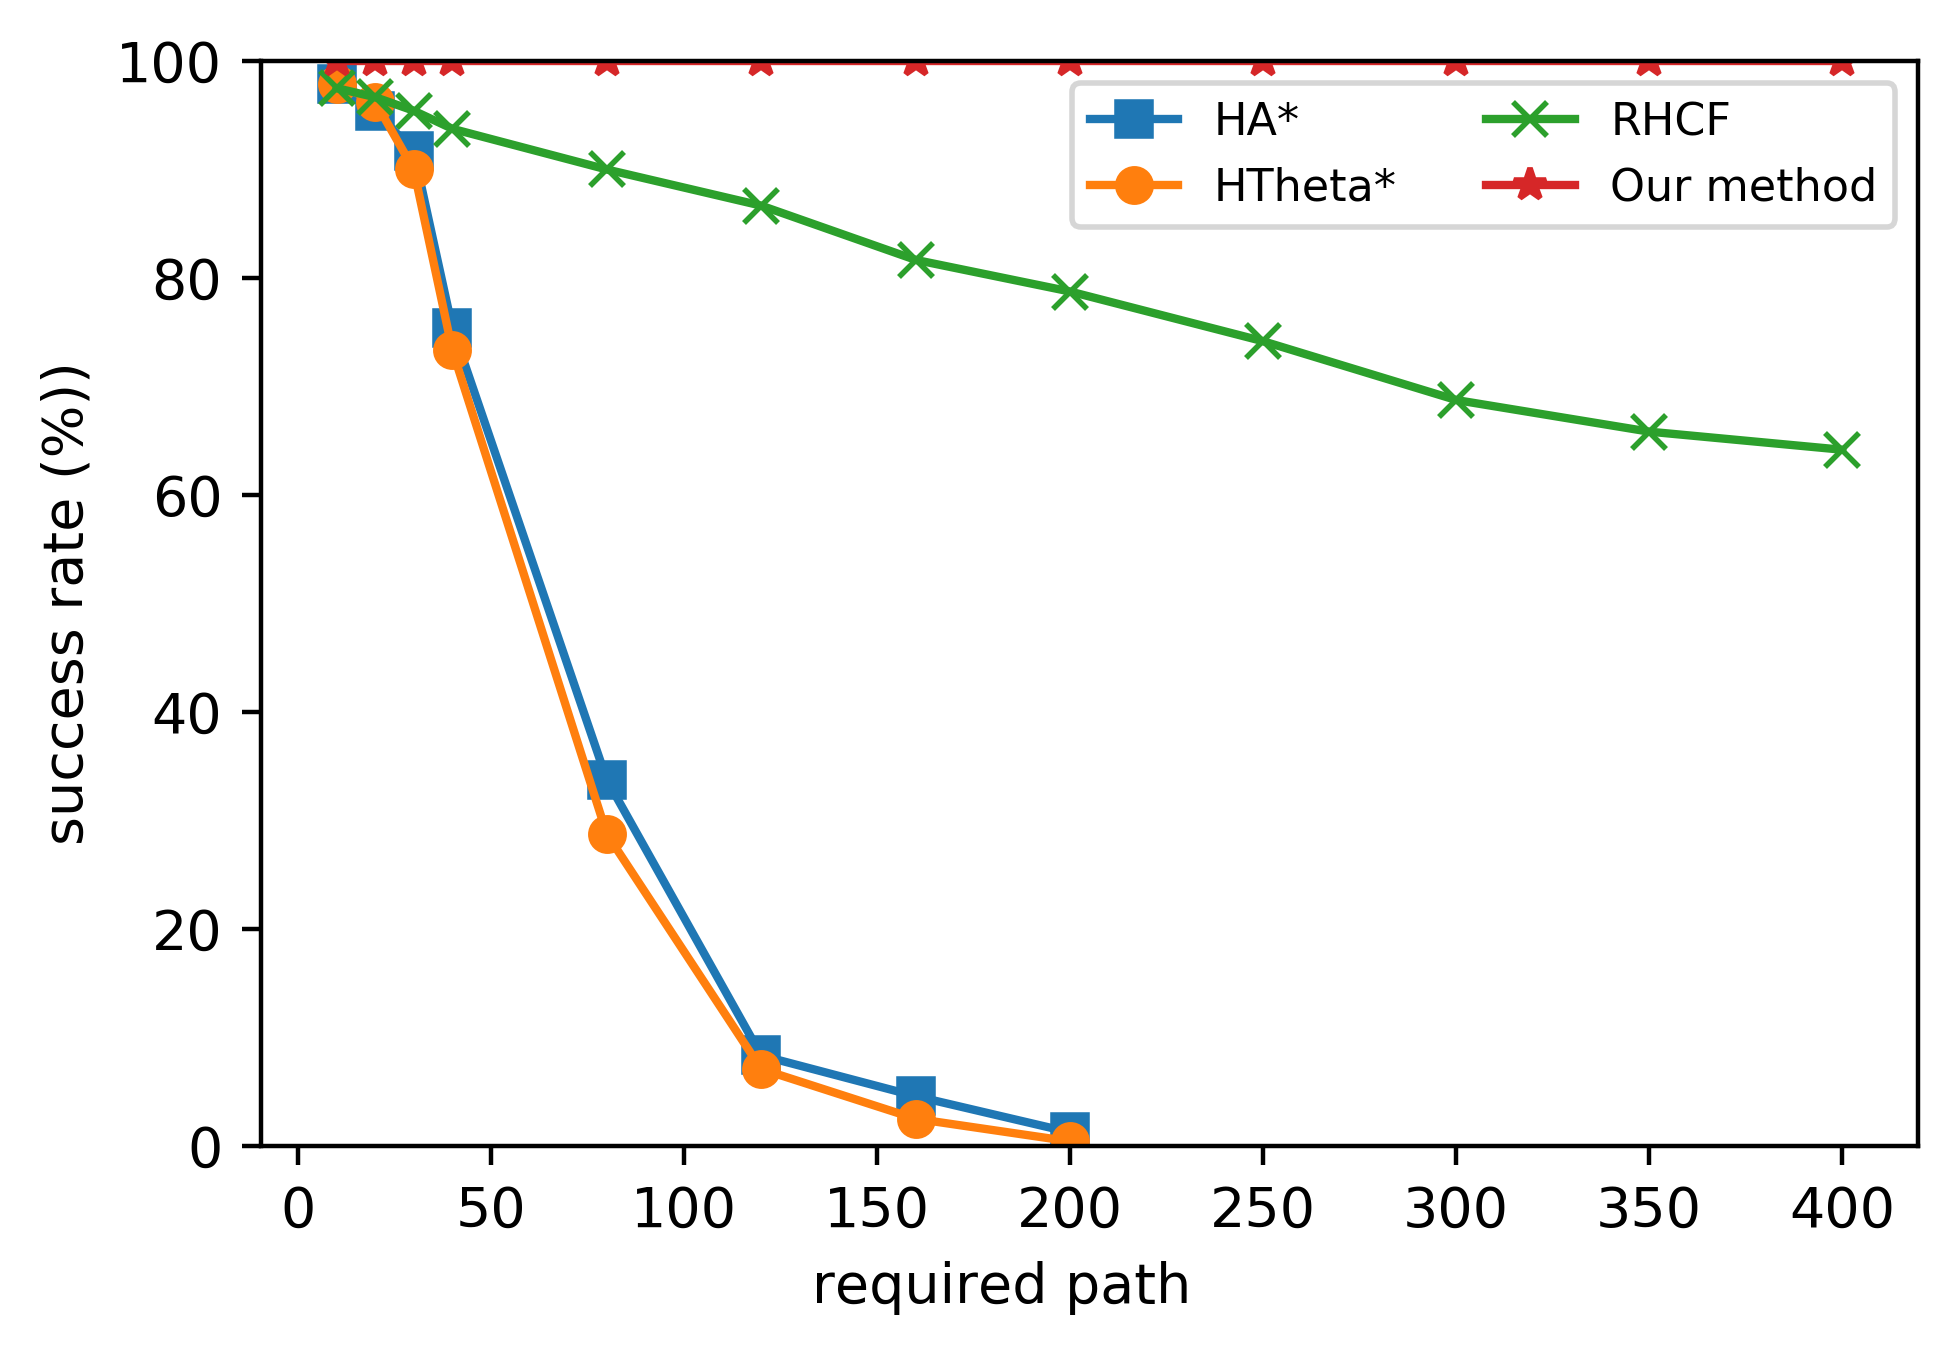
\includegraphics[width=4.6cm]{comparison_succ_and_count.png}}
  \centerline{B: success rate comparison}
\end{minipage}
\vfill

\caption{These figures show the comparison of the success rates and time costs of the four methods across all eight maps, with a consistent magnification set to 1.0.}
\label{compariosn_between_methods}
\end{figure}


%Firstly, we test all four methods under the mentioned eight maps, use them to find multiple (range from 10 to 400) topologically distinctive paths, and we recorded the mean time cost and success rate under each maps, as shown in Fig. \ref{total_time_cost_and_path_count} and Fig. \ref{succ_and_path_count} respectively. The combined results of time cost and success rate are shown in Fig. \ref{compariosn_between_methods}.

%As shown in Fig. \ref{total_time_cost_and_path_count} and Fig. \ref{succ_and_path_count}, our method's mean time cost to find 400 paths is 500ms approximately, and its success rate is 100\%. While for RHCF, it take approximately 7s to find 400 paths in average under the worst case and its success rate is decrease to 80\% in the best case and 40\% in the worst case. For HA* and HTheta*, their mean time cost is close to the time upper bound (10s) when try to find more than 80 paths. And their success rate decreases as mean time cost increases, it decreases to 50\% after try to find more than 40 paths.   And our method's time cost increase in a slower way than other methods, as our method avoid mutiple graph search for multiple path but get all required paths during one times of search. Out method only take 500ms in average in the worst case, and always are 100\% to find required number of paths.

%In this section, our method demostrate overwhelming advantage to other methods in term of time cost and success rate. 

Initially, we subjected all four methods to testing under the specified eight maps, utilizing them to search varying numbers of topologically distinctive paths (ranging from 10 to 400). The mean time cost and success rate were recorded for each map, as depicted in Fig. \ref{total_time_cost_and_path_count} and Fig. \ref{succ_and_path_count} respectively. The amalgamated results, showcasing the interplay between time cost and success rate, are illustrated in Fig. \ref{compariosn_between_methods}.

As illustrated in Fig. \ref{total_time_cost_and_path_count} and Fig. \ref{succ_and_path_count}, our method achieves a mean time cost of approximately 500ms to find 400 paths, boasting a 100\% success rate. In contrast, RHCF takes around 7s to find 400 paths on average, with its success rate varying from 80\% in the best case to 40\% in the worst case. For HA* and HTheta*, their mean time cost approaches the time upper bound (10s) when attempting to find more than 80 paths. Moreover, their success rate declines as the mean time cost increases, dropping to 50\% after attempting to find more than 40 paths. Notably, our method exhibits a slower increase in time cost compared to other methods, as it circumvents multiple graph searches for multiple paths, obtaining all required paths in a single search. With an average time cost of only 500ms in the worst case, our method consistently achieves a 100\% success rate in finding the required number of paths.

This section underscores our method's substantial advantage over other methods in terms of time cost and success rate.

\subsubsection{Path length}

% time and scale
\begin{figure*}[t] \scriptsize
%\begin{tabular}{cc}
\begin{minipage}{.245\linewidth}
  \centerline{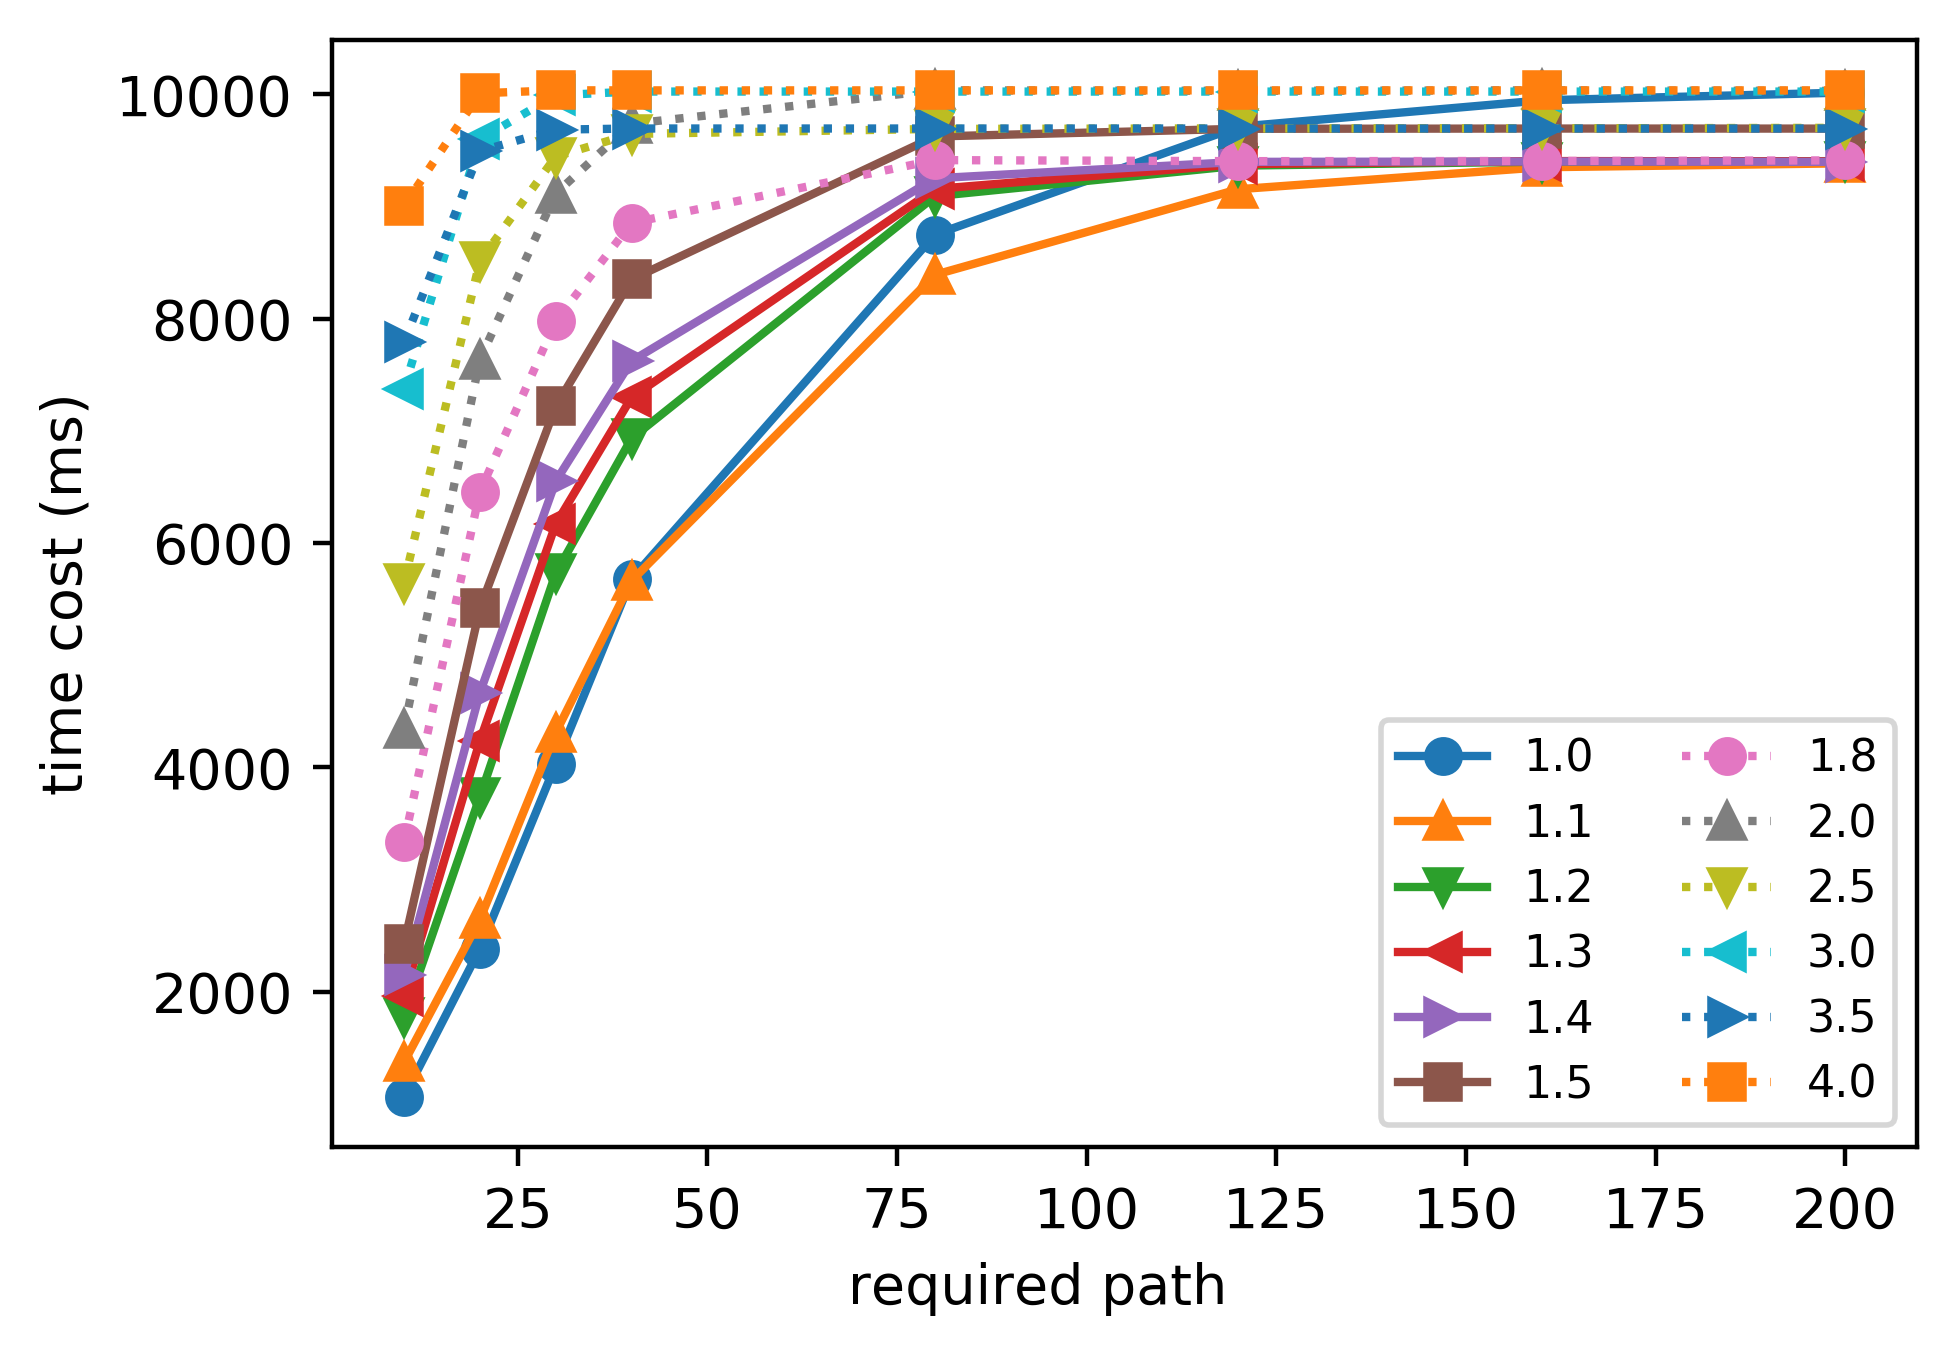
\includegraphics[width=4.6cm]{HsAs_scale_cost_method_path_count.png}}
  \centerline{A: HA*}
\end{minipage}
\hfill
\begin{minipage}{.245\linewidth}
  \centerline{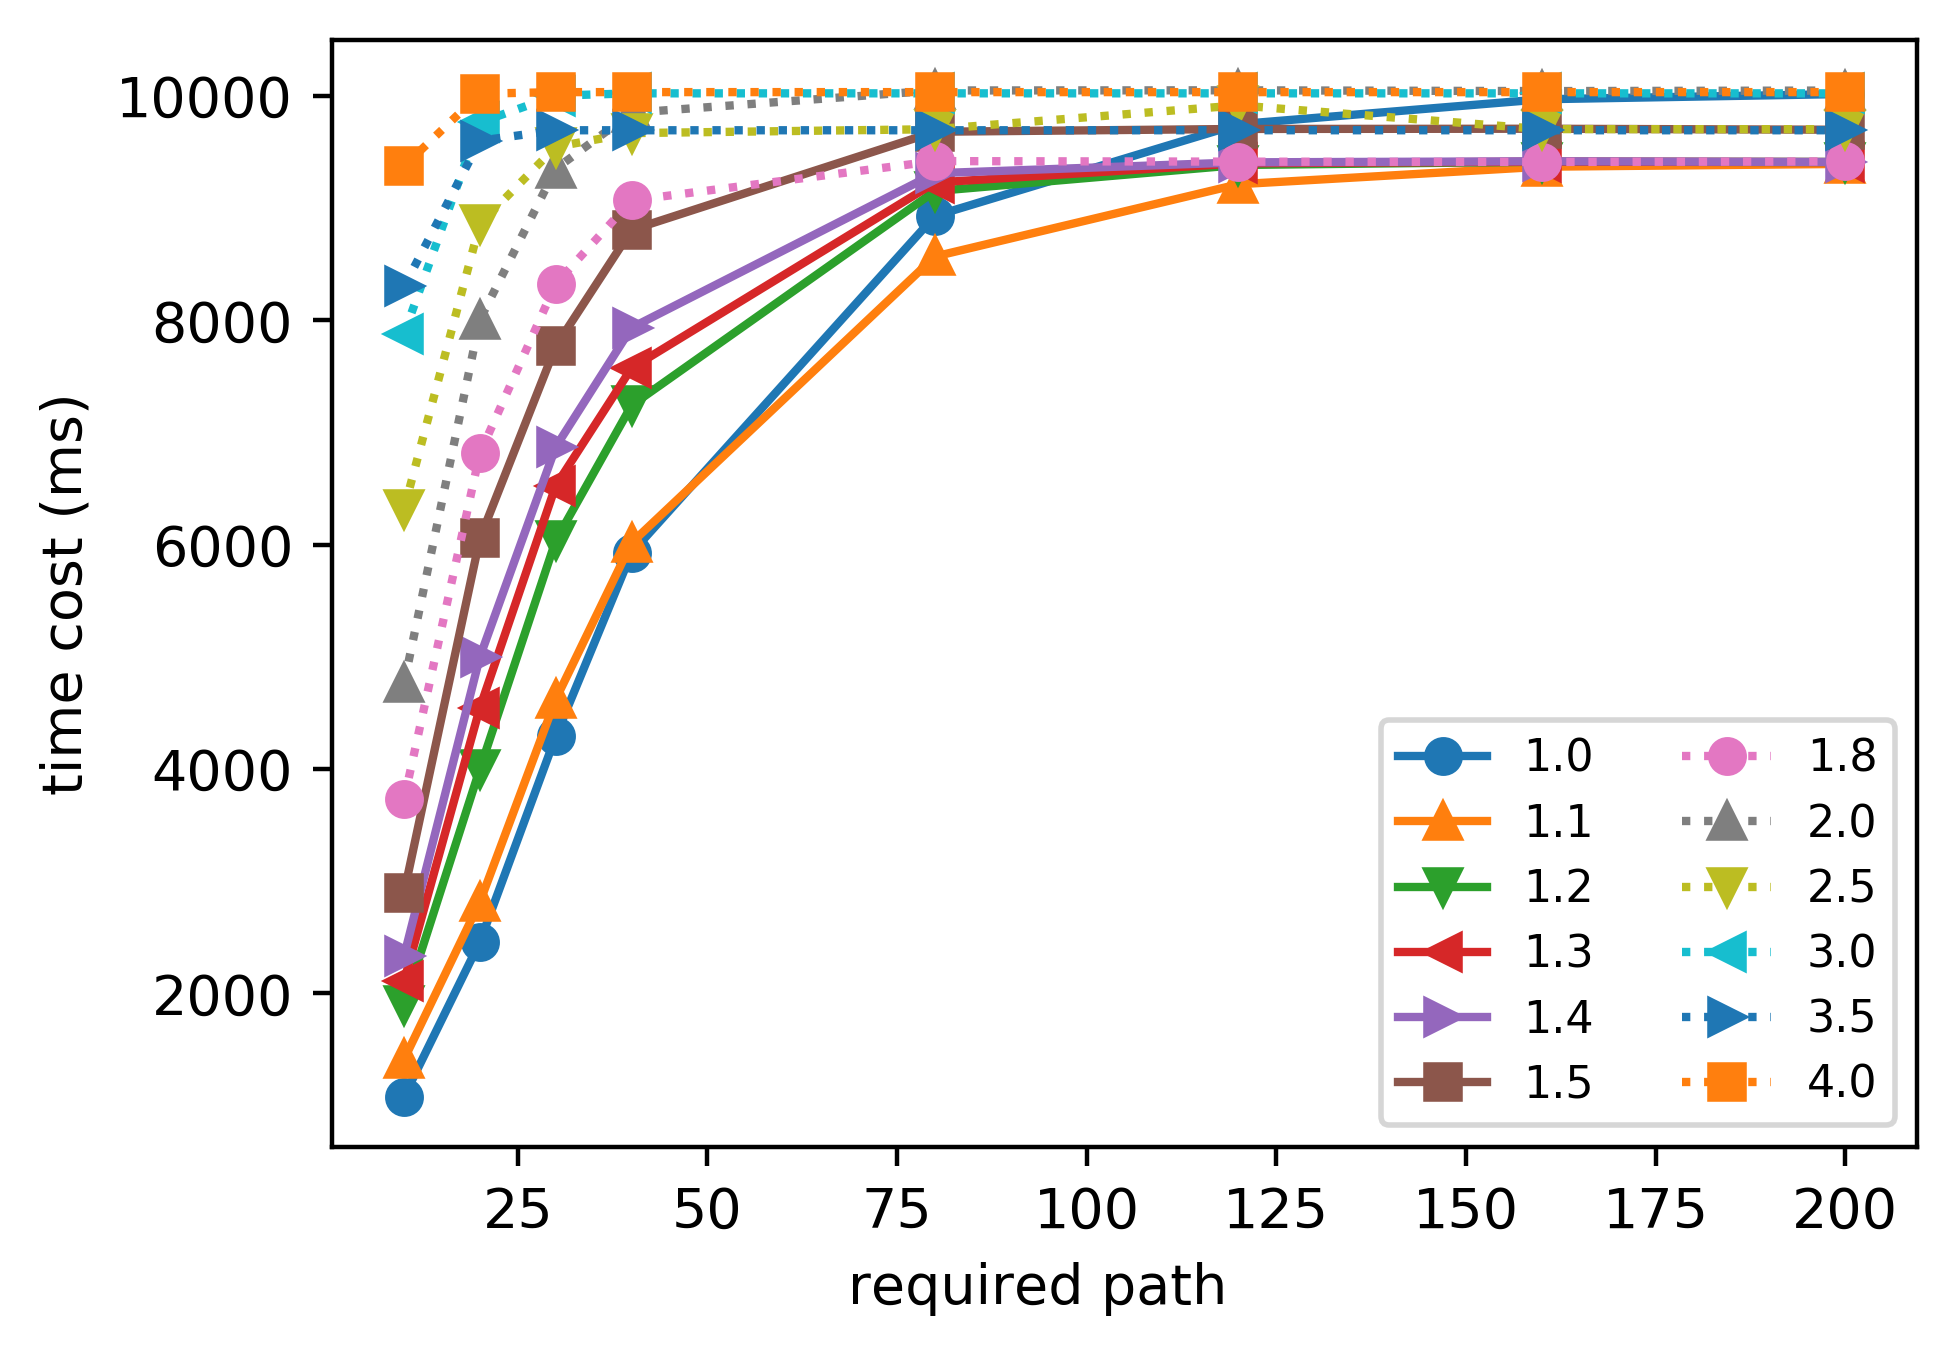
\includegraphics[width=4.6cm]{HsTs_scale_cost_method_path_count.png}}
  \centerline{B: HTheta*}
\end{minipage}
\hfill
\begin{minipage}{.245\linewidth}
  \centerline{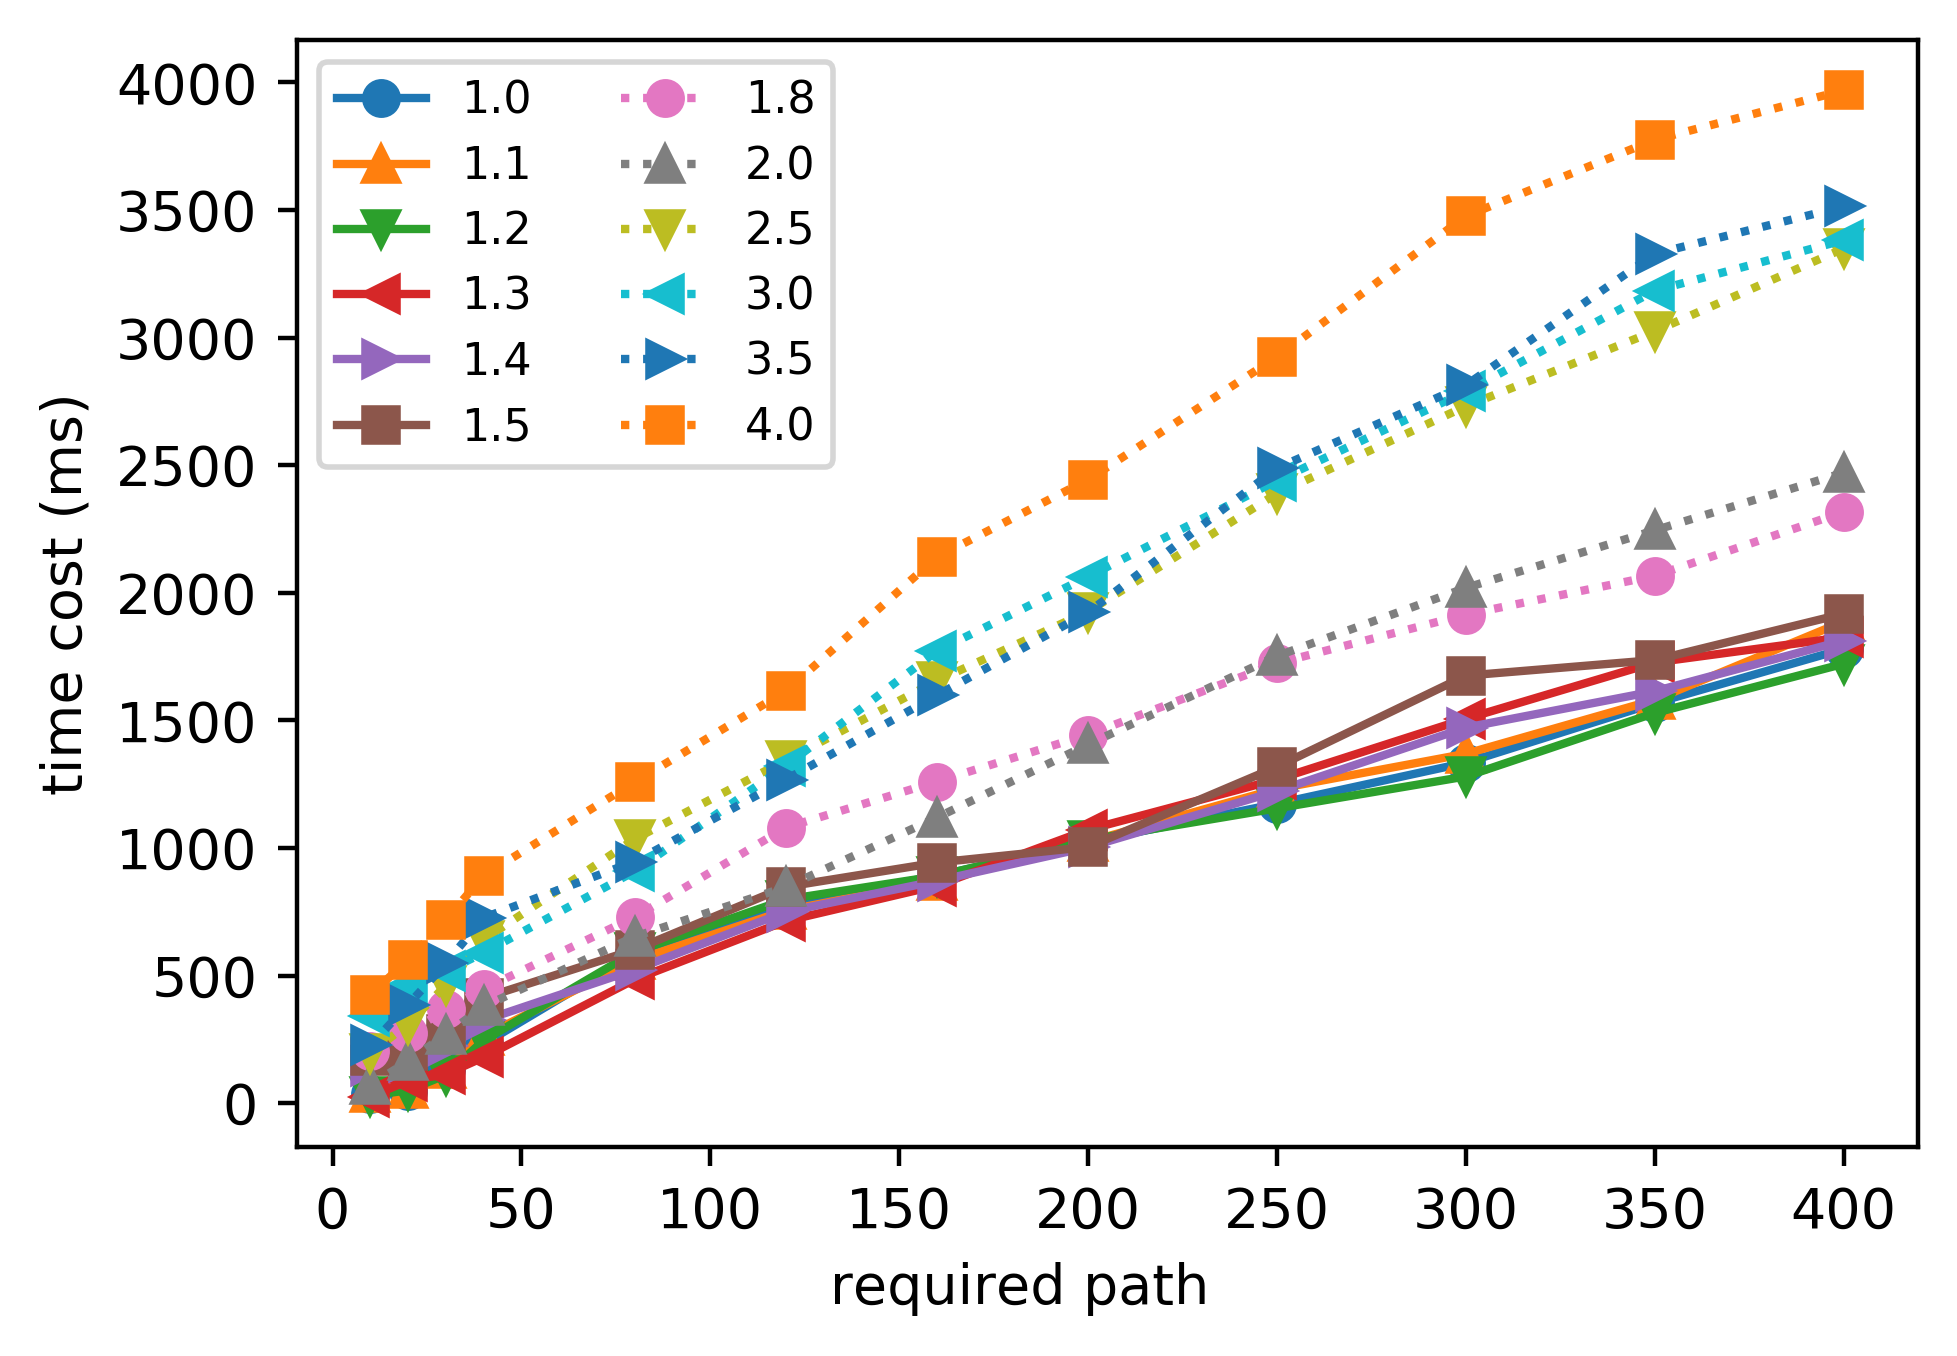
\includegraphics[width=4.6cm]{RHCF_scale_cost_method_path_count.png}}
  \centerline{C: RHCF}
\end{minipage}
\hfill
\begin{minipage}{.245\linewidth}
  \centerline{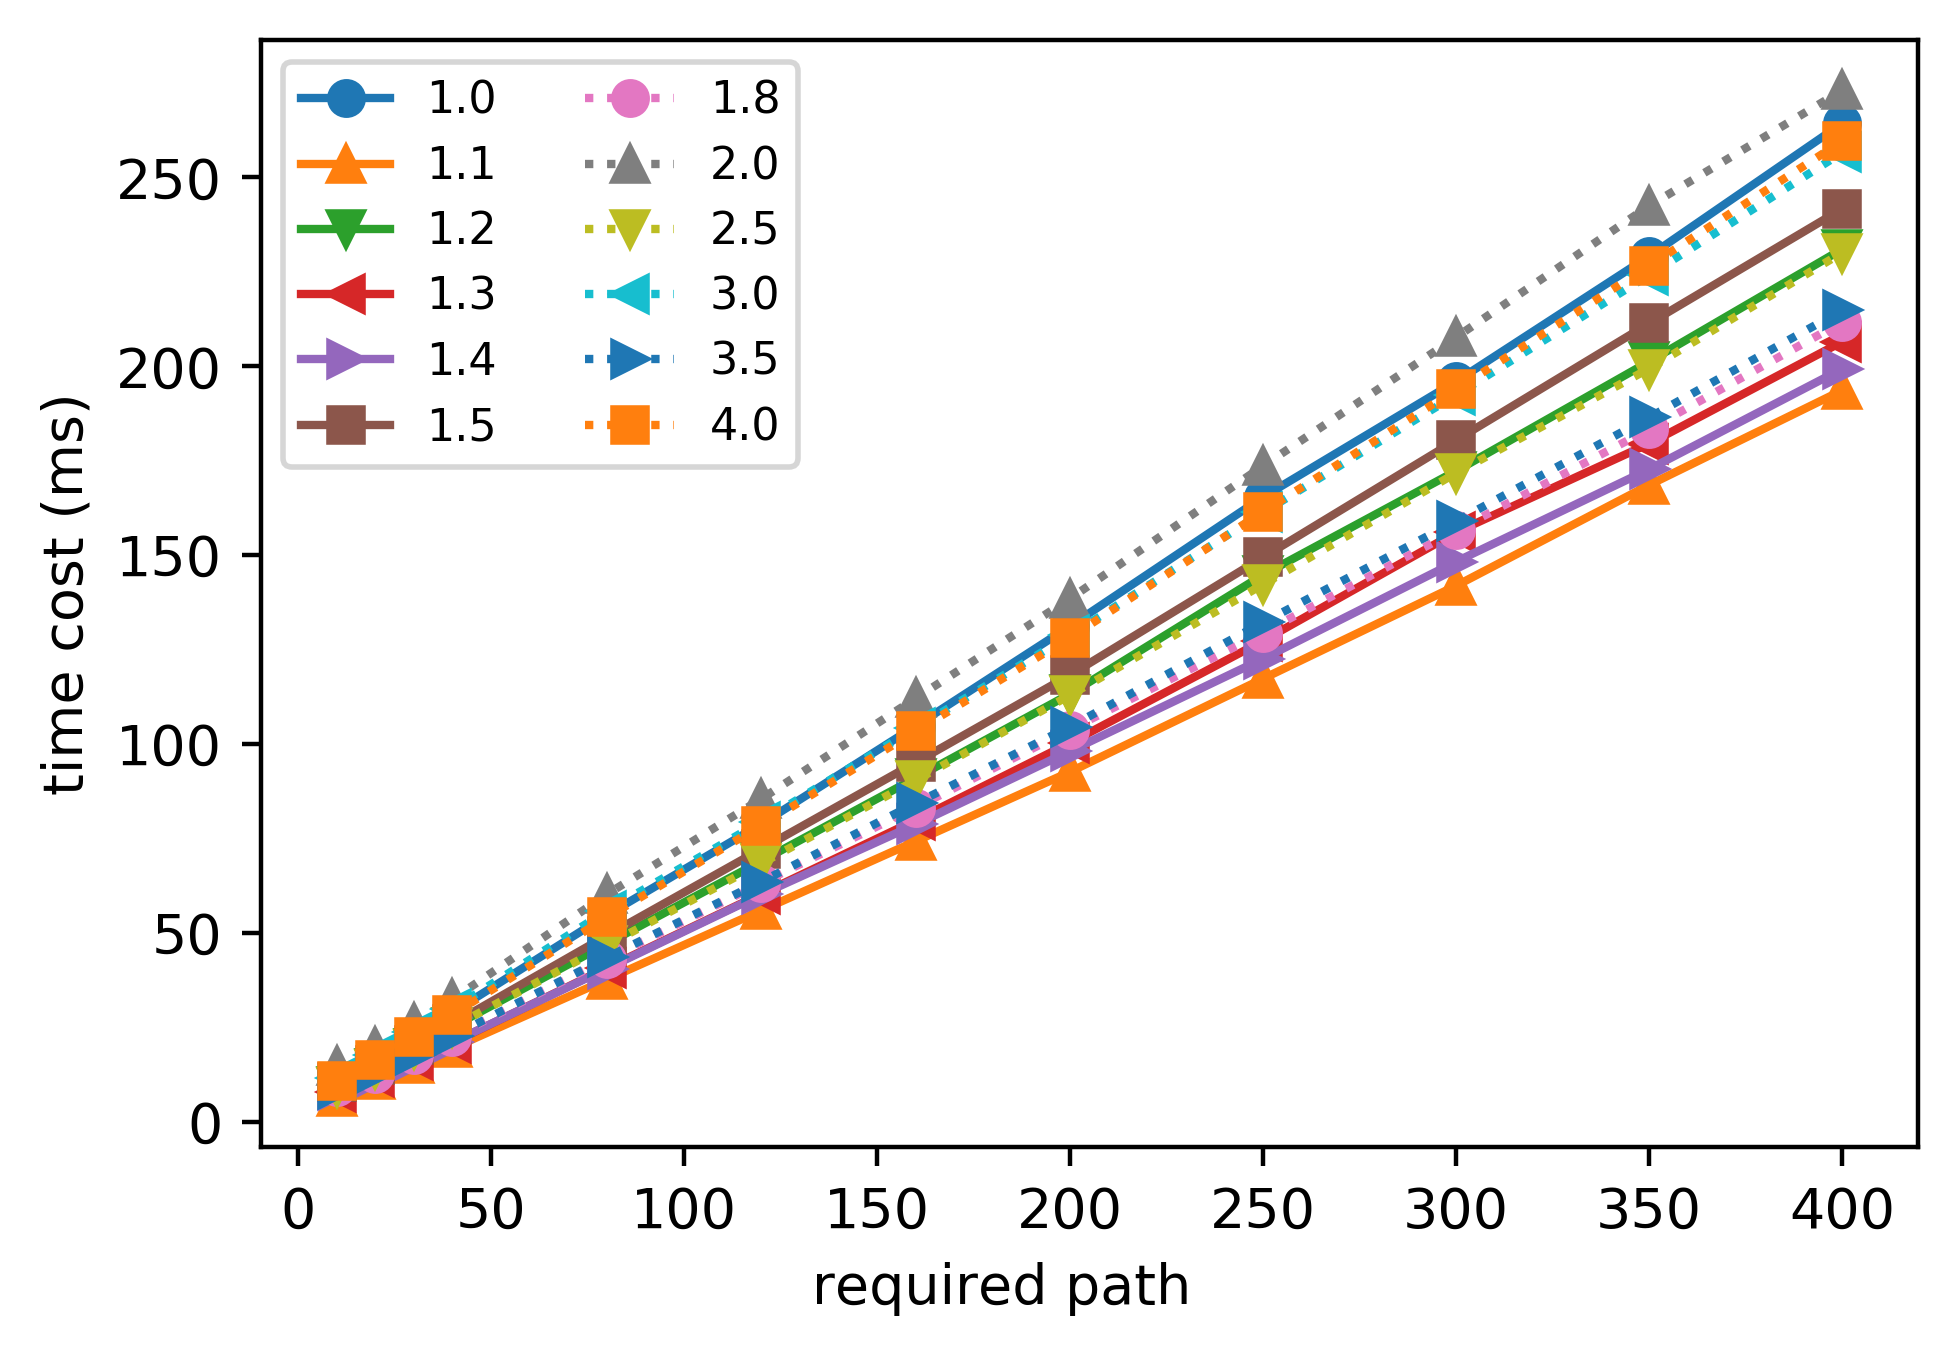
\includegraphics[width=4.6cm]{RJ_scale_cost_method_path_count.png}}
  \centerline{D: Our method}
\end{minipage}
\vfill

\caption{These figures illustrate that the mean time cost to find the required number of paths increases with the magnification of the maps, covering all eight maps.}
\label{scale_cost_method_path_count}
\end{figure*}

% success rate and scale
\begin{figure*}[t] \scriptsize
%\begin{tabular}{cc}
\begin{minipage}{.245\linewidth}
  \centerline{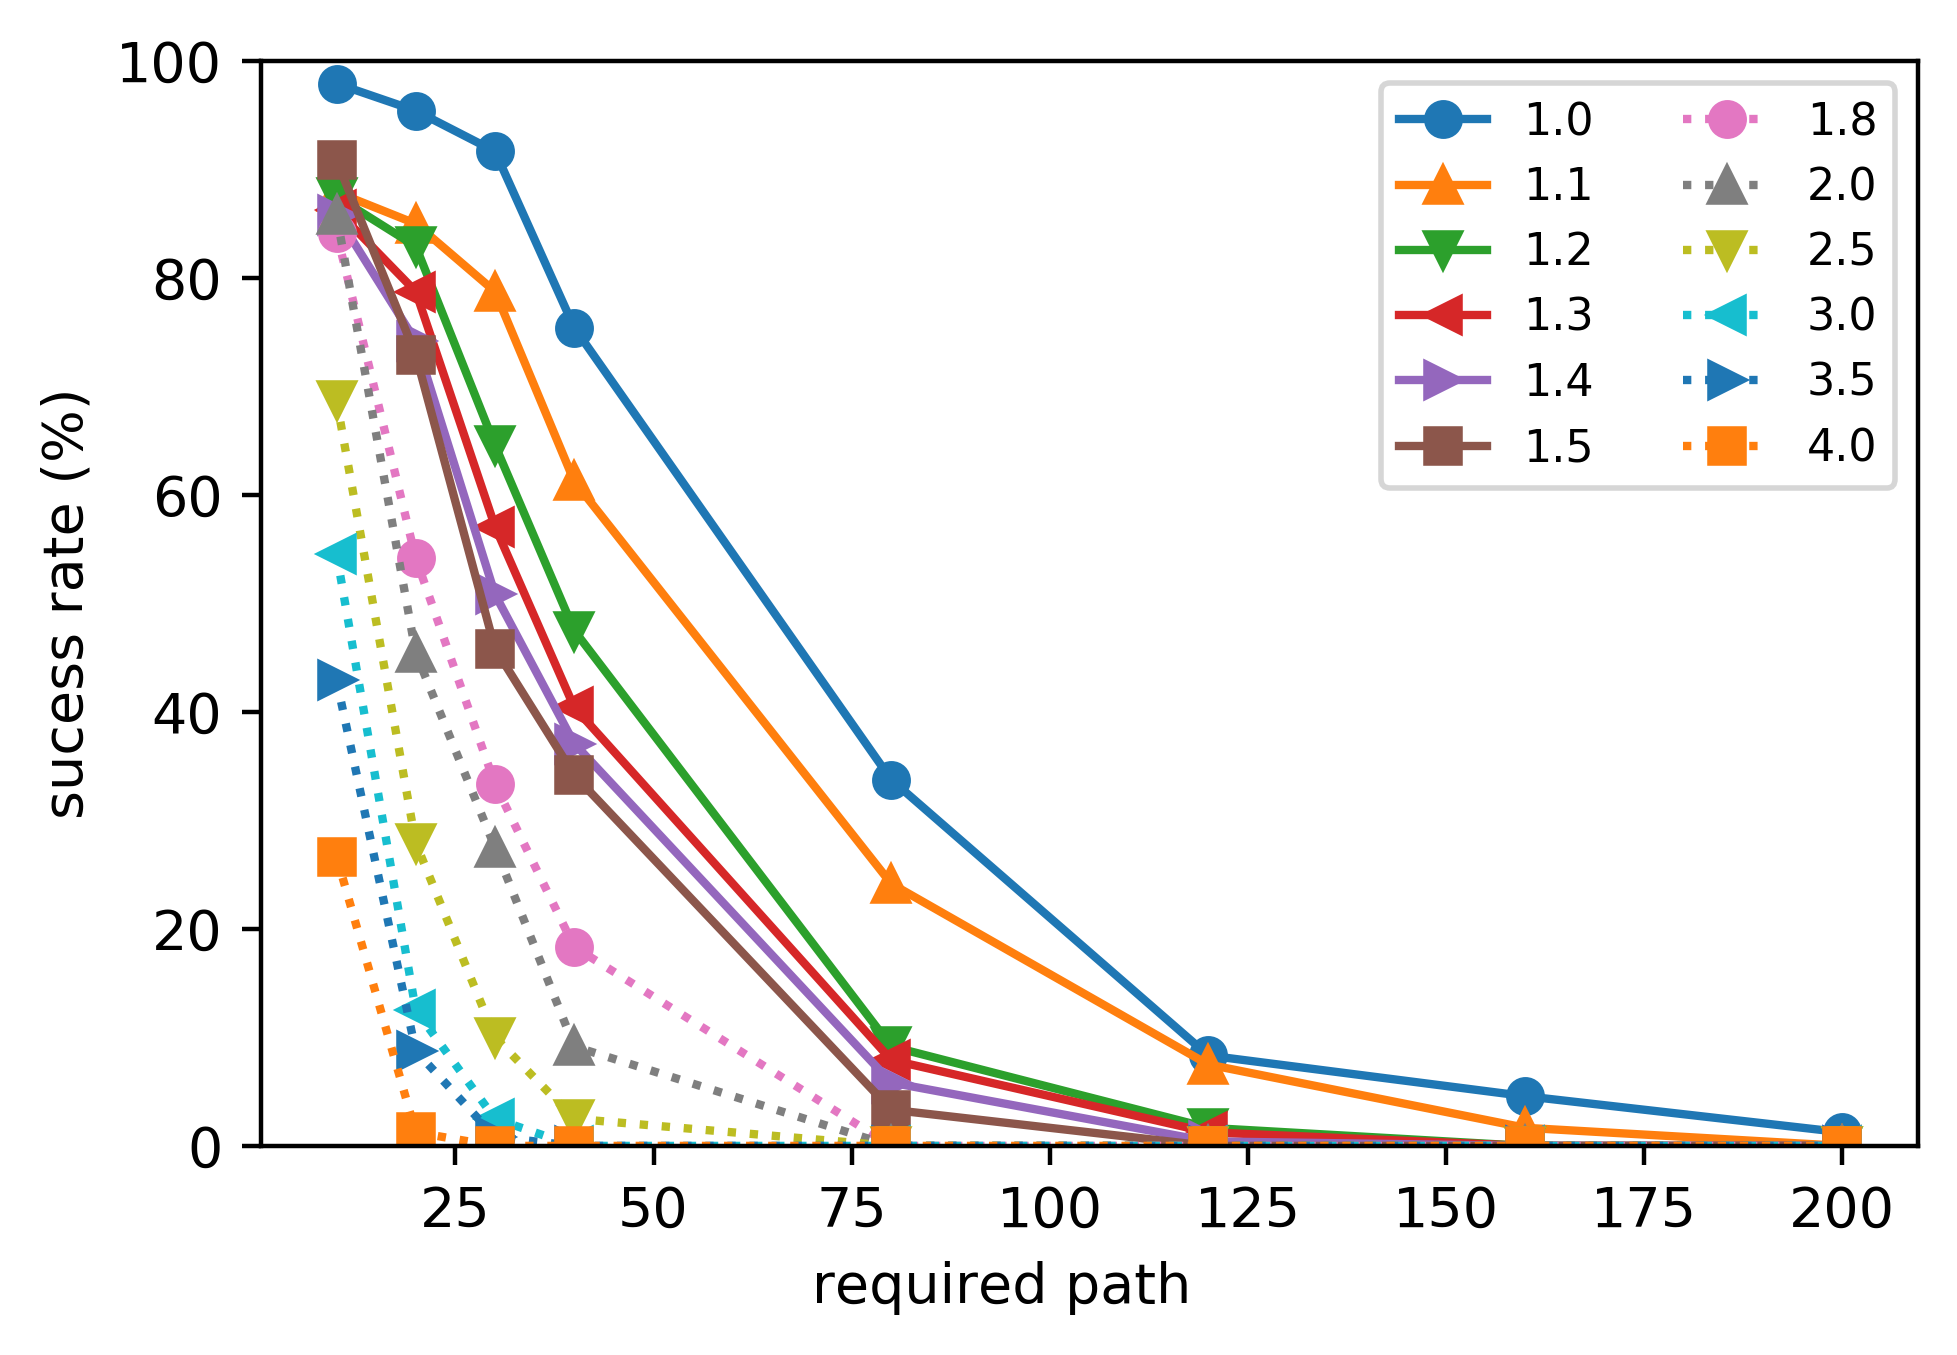
\includegraphics[width=4.6cm]{HsAs_scale_succ_method_path_count.png}}
  \centerline{A: HA*}
\end{minipage}
\hfill
\begin{minipage}{.245\linewidth}
  \centerline{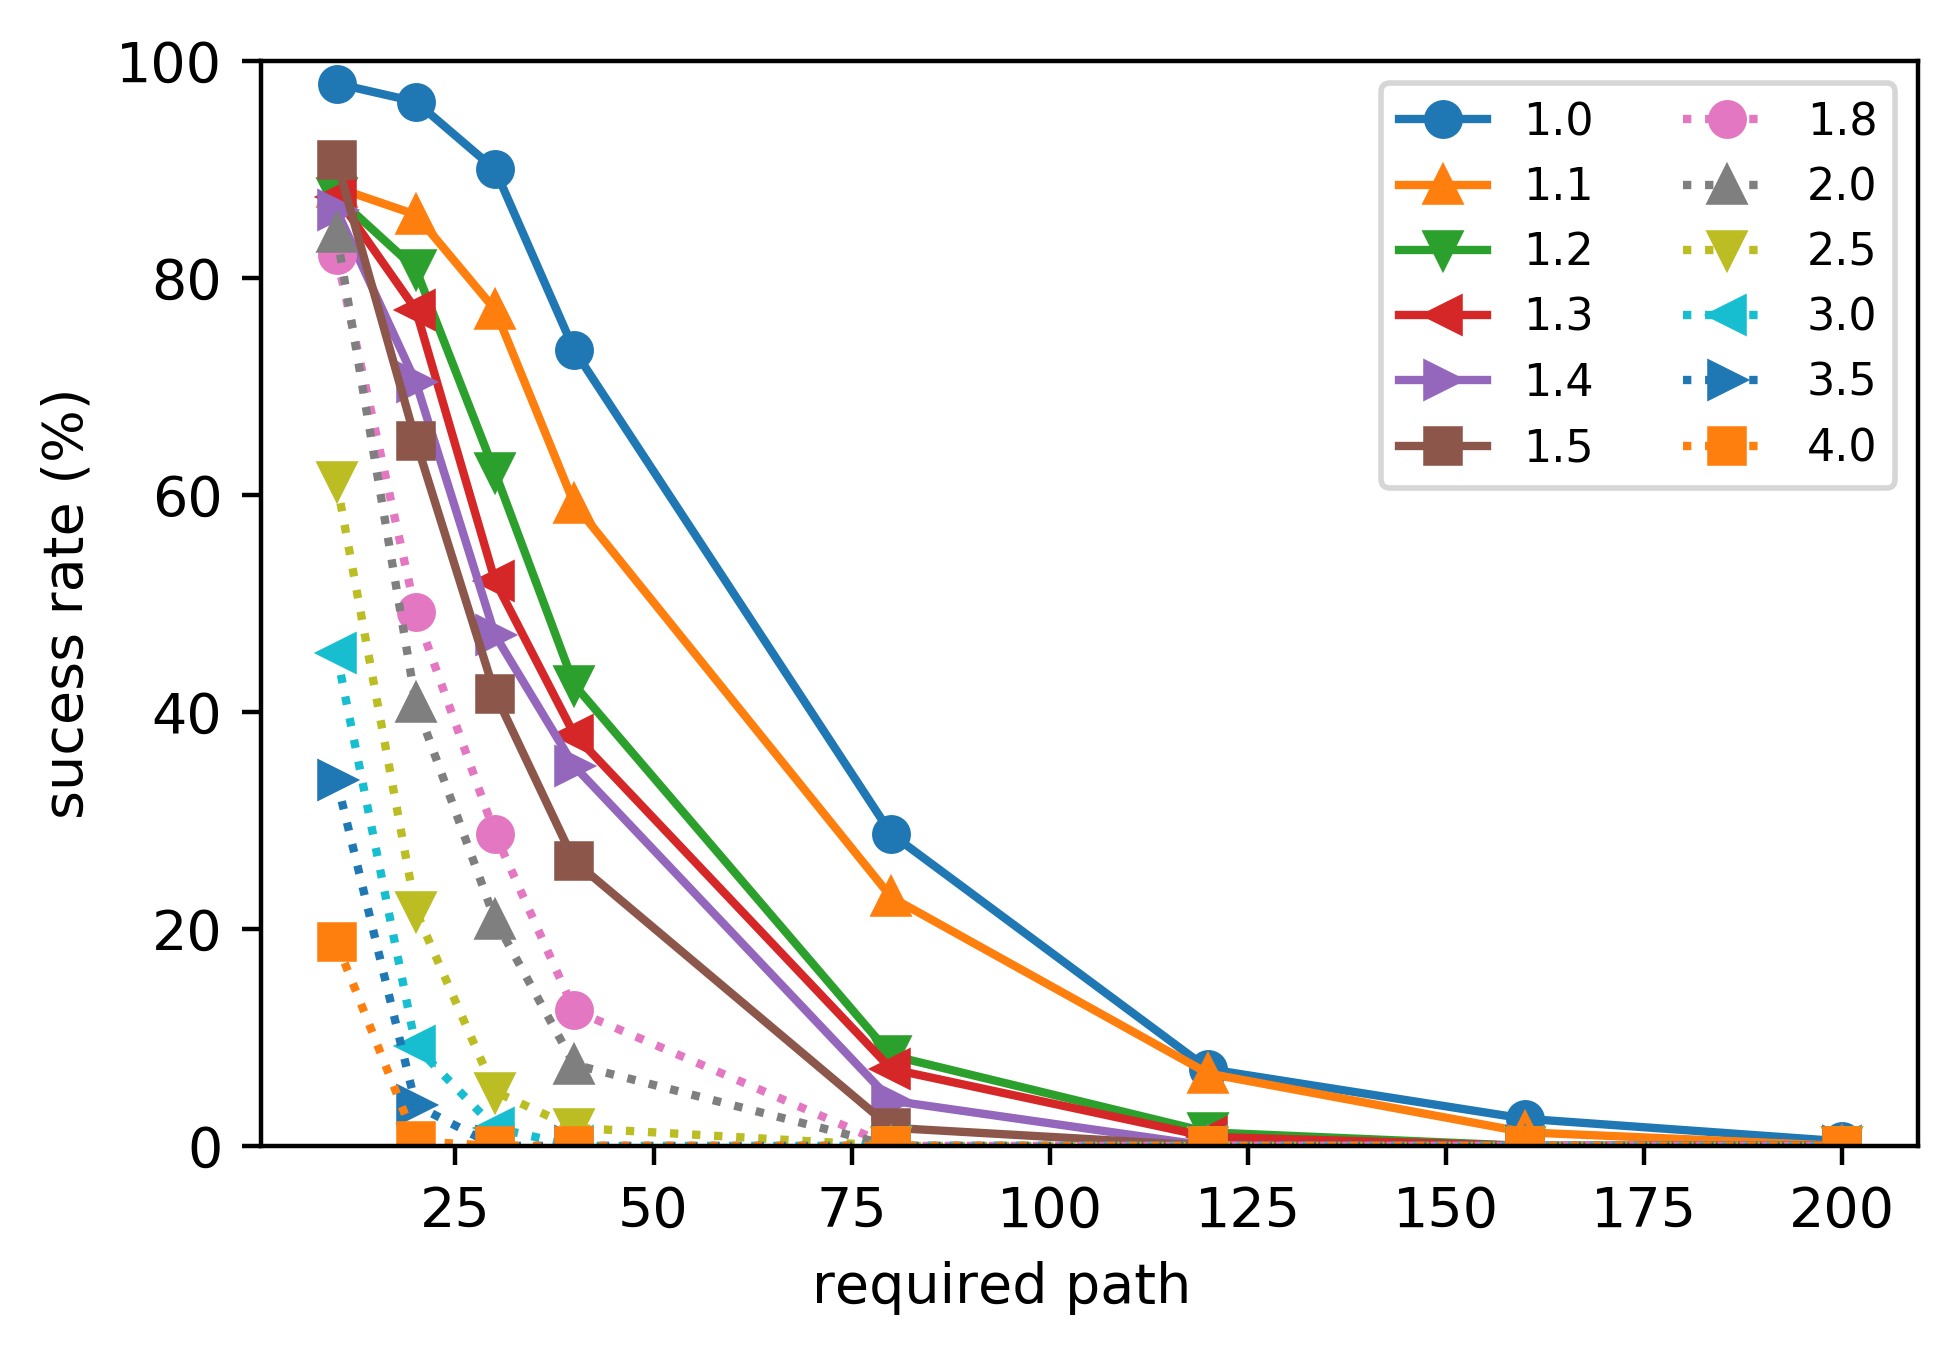
\includegraphics[width=4.6cm]{HsTs_scale_succ_method_path_count.png}}
  \centerline{B: HTheta*}
\end{minipage}
\hfill
\begin{minipage}{.245\linewidth}
  \centerline{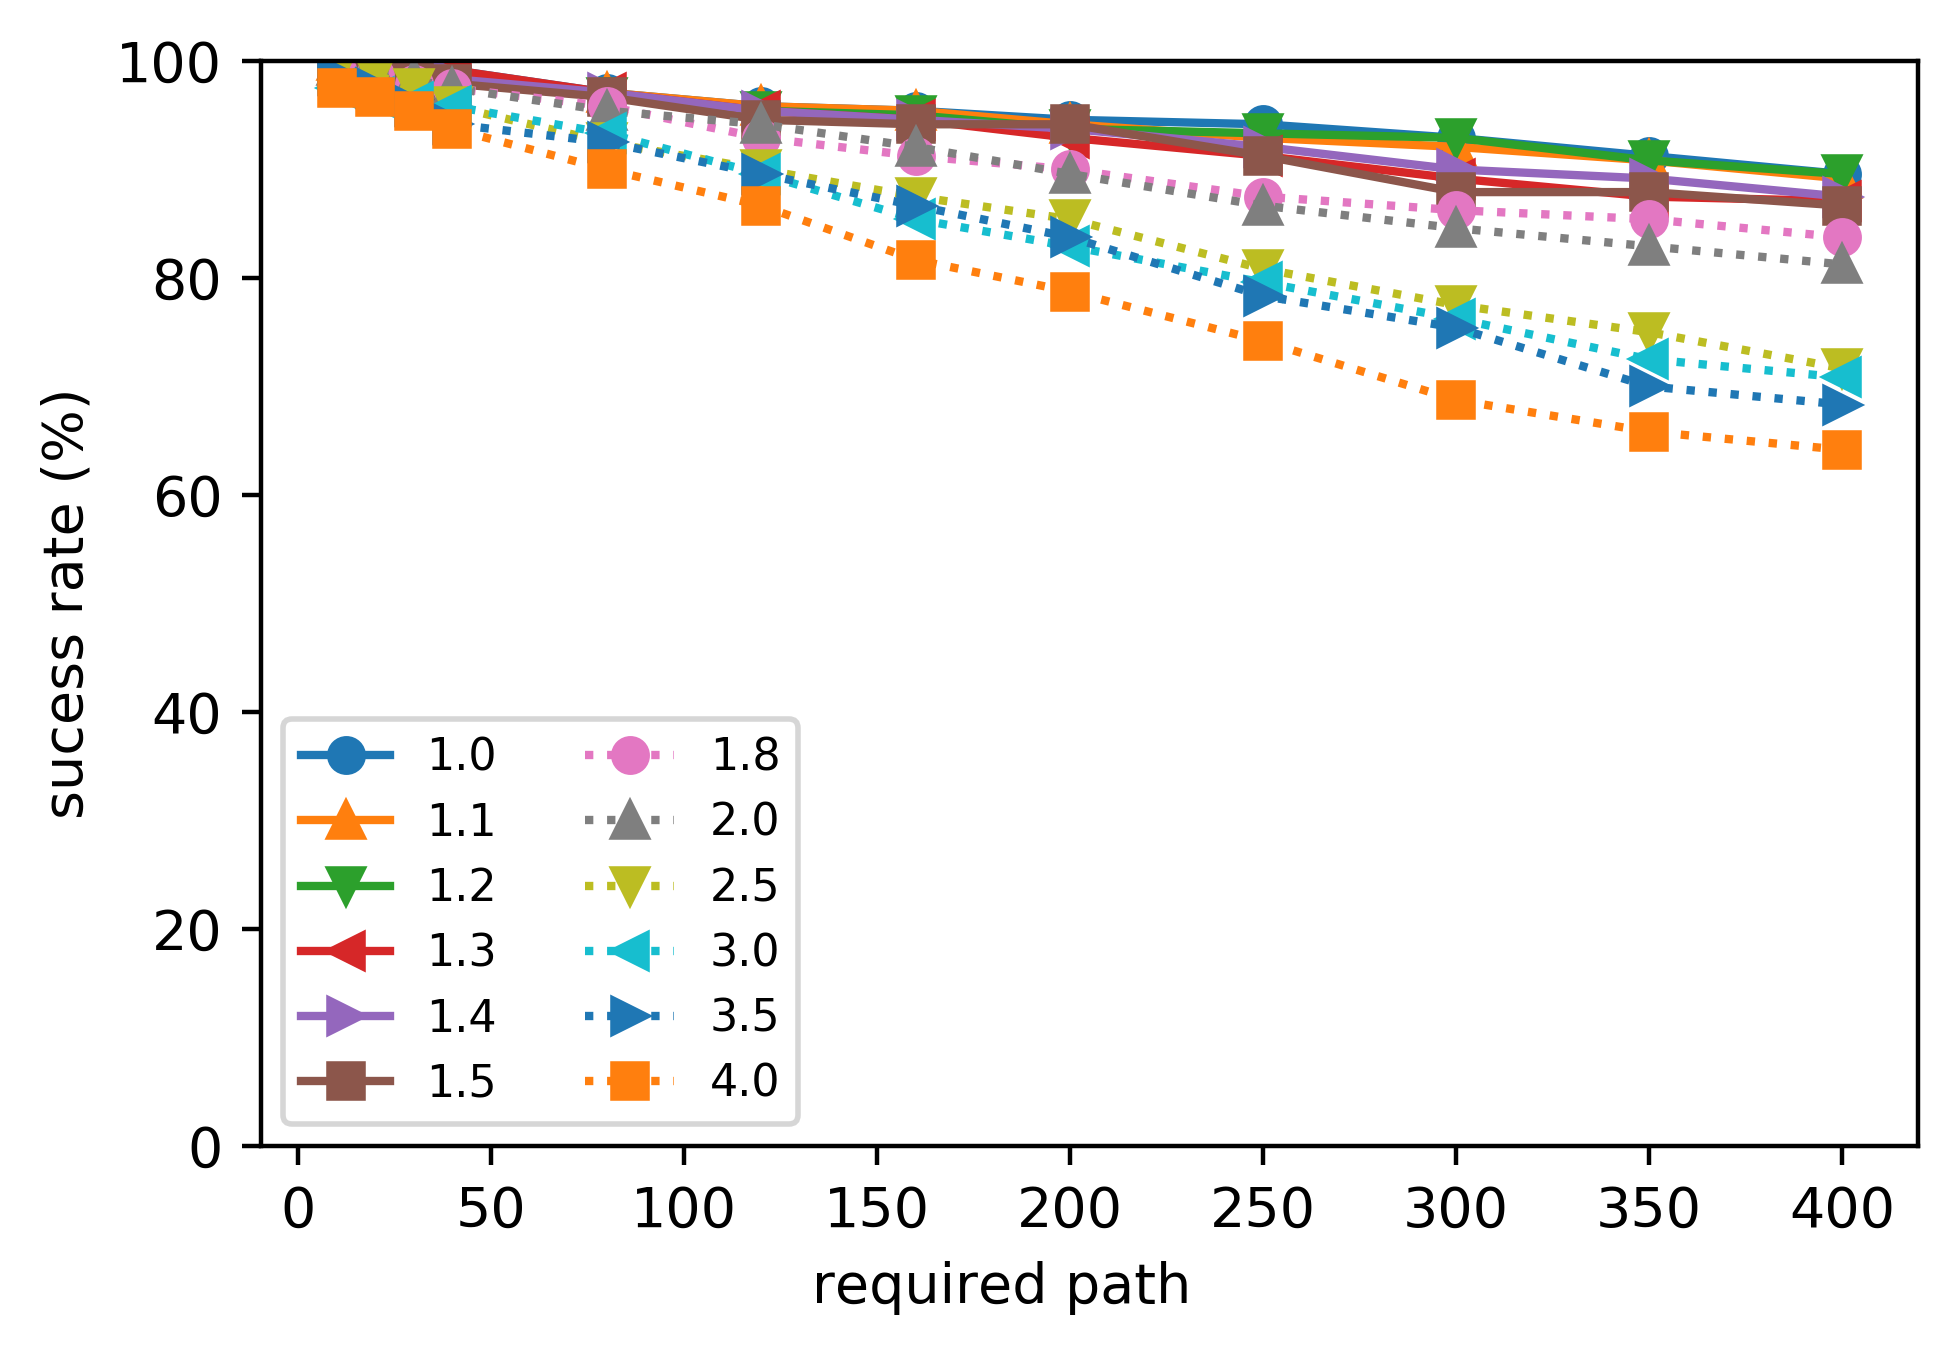
\includegraphics[width=4.6cm]{RHCF_scale_succ_method_path_count.png}}
  \centerline{C: RHCF}
\end{minipage}
\hfill
\begin{minipage}{.245\linewidth}
  \centerline{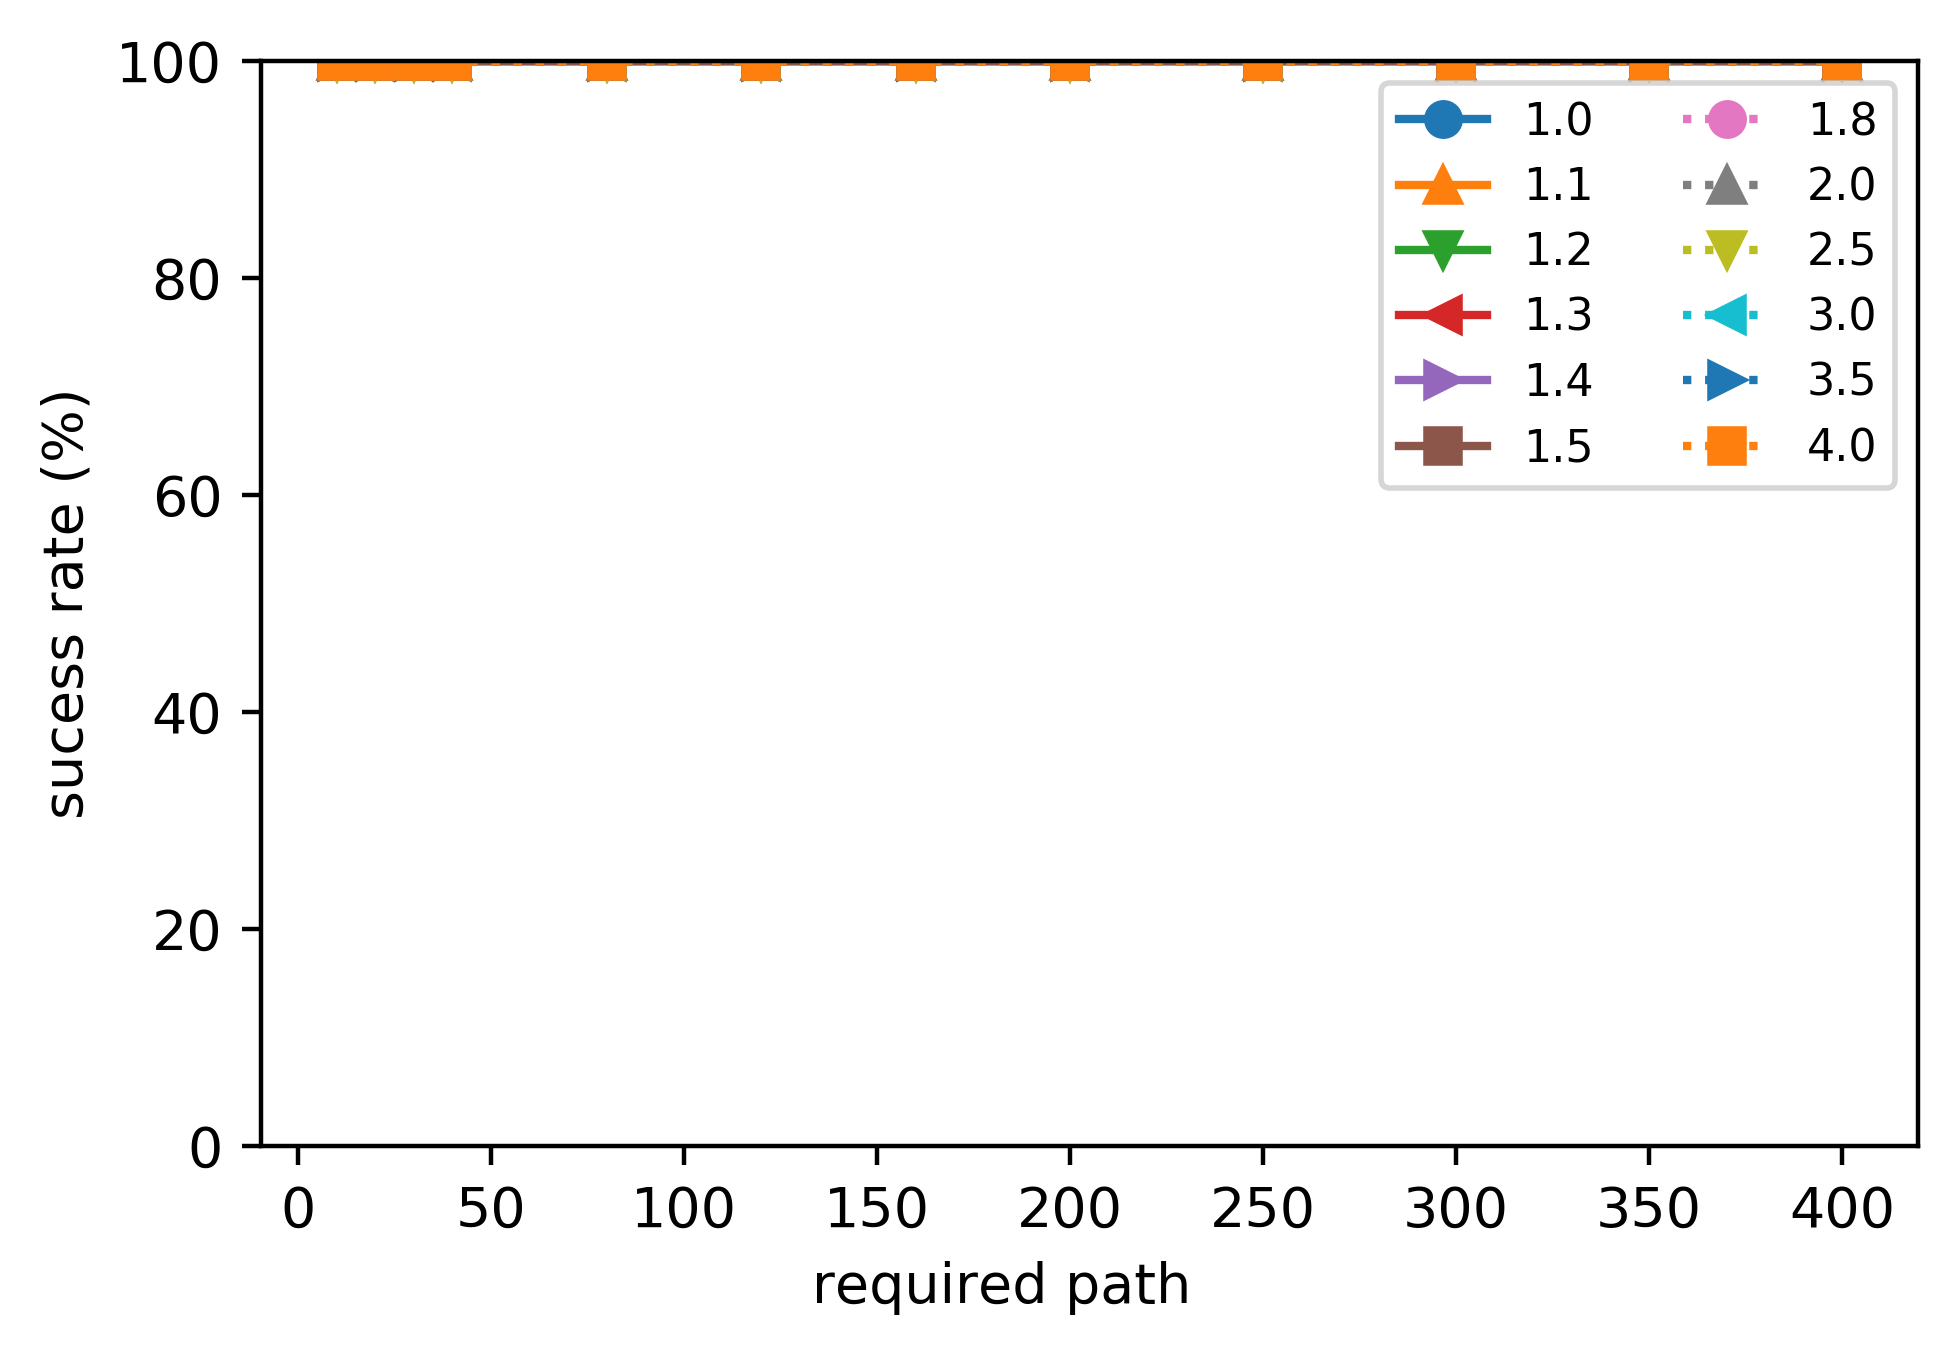
\includegraphics[width=4.6cm]{RJ_scale_succ_method_path_count.png}}
  \centerline{D: Our method}
\end{minipage}
\vfill

\caption{These figures illustrate that the mean success rate to find the required number of paths increases with the magnification of the maps, covering all eight maps.}
\label{scale_succ_method_path_count}
\end{figure*}

\begin{figure}[t] \scriptsize
%\begin{tabular}{cc}
  \centerline{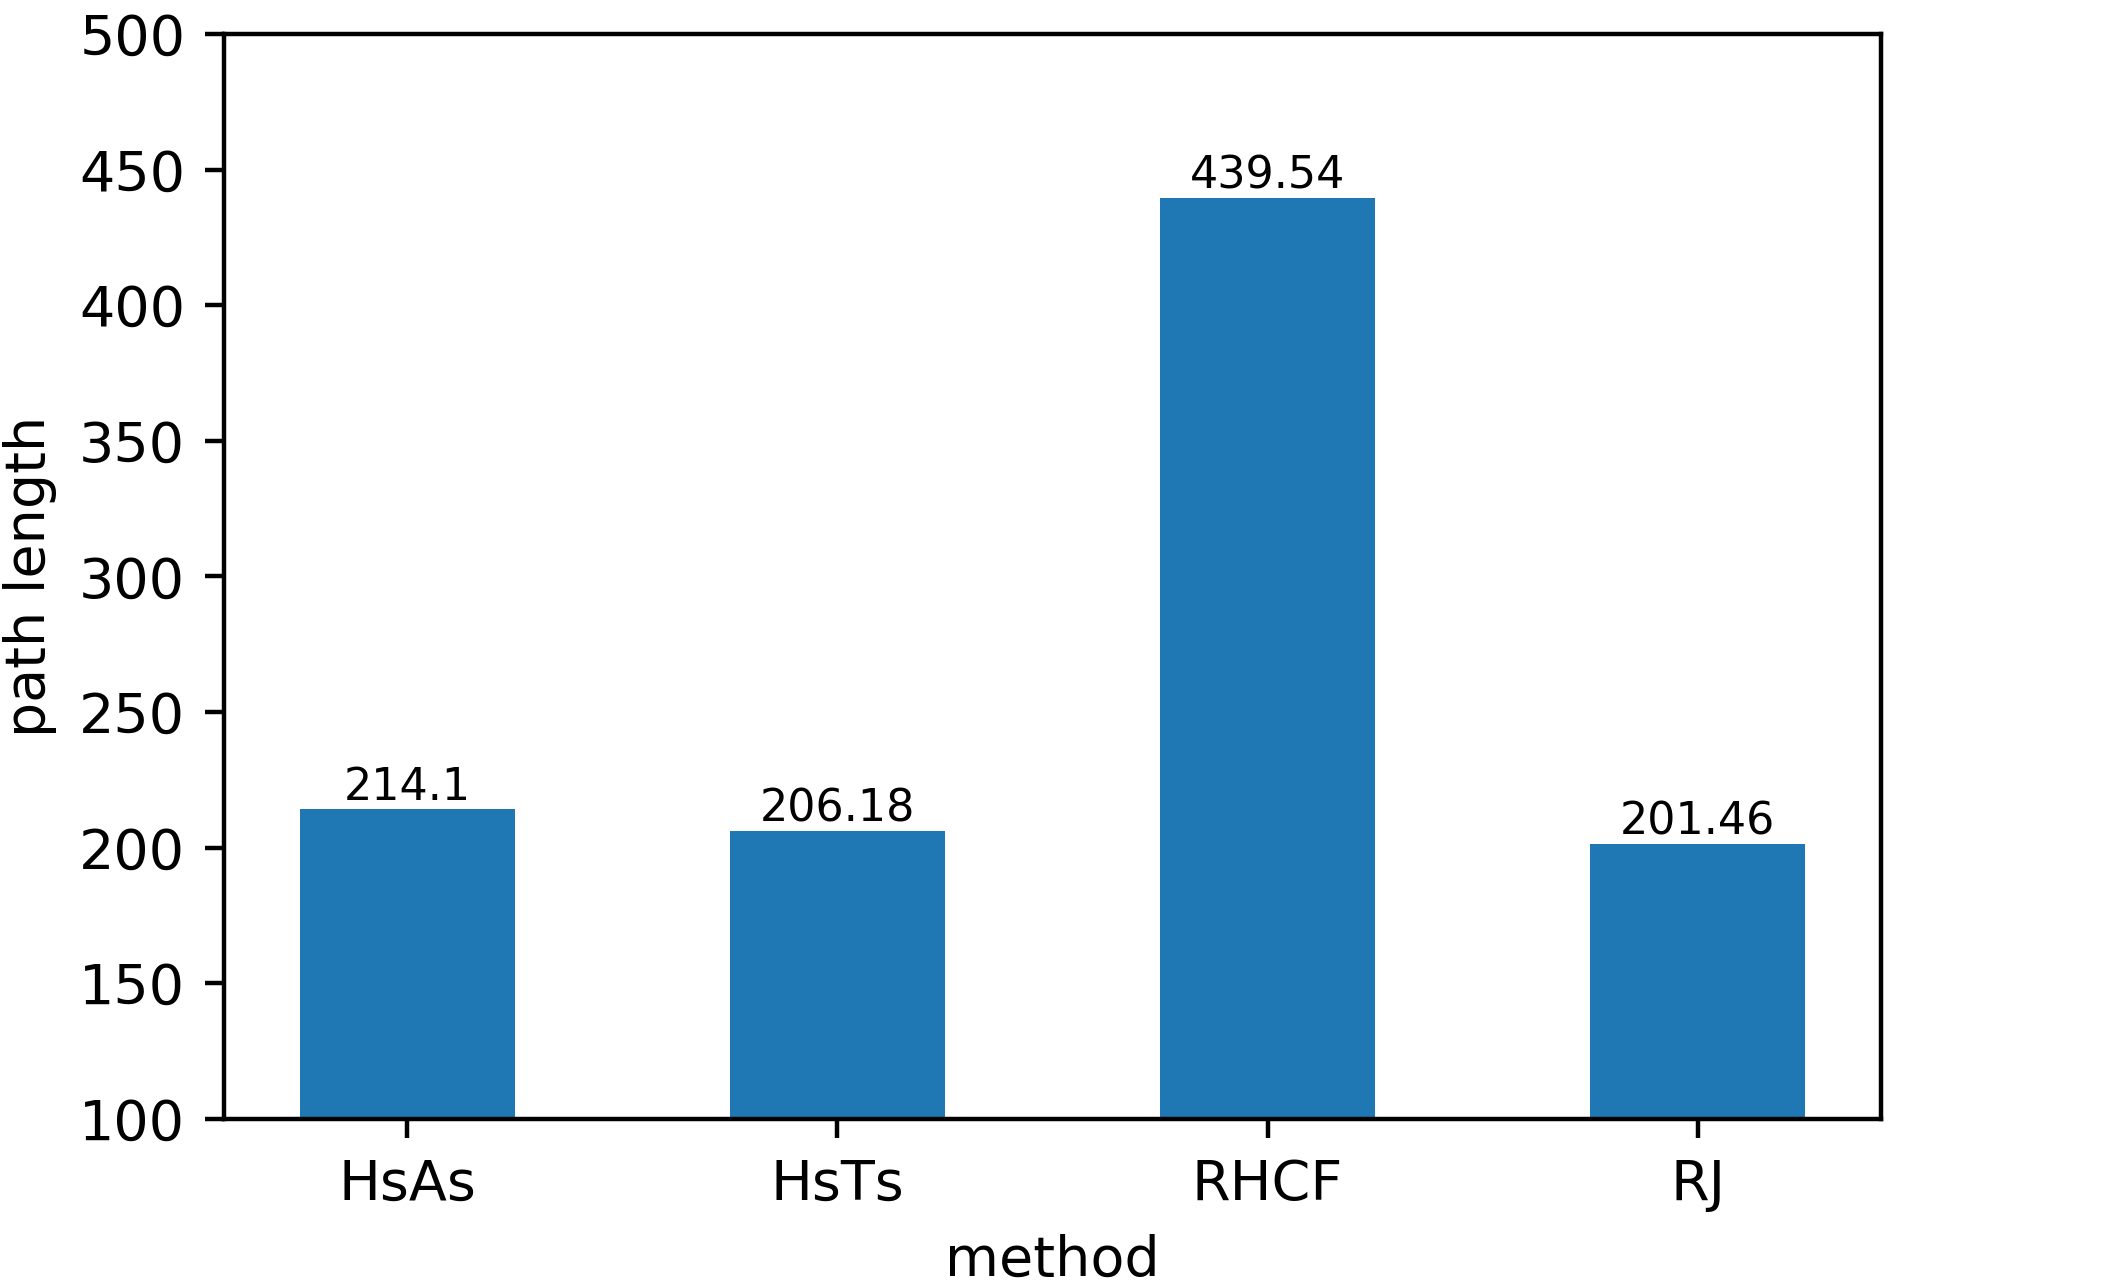
\includegraphics[width=4.6cm]{method_path_length.png}}
  \centerline{mean path length comparison}
\caption{These figures present a comparison of path lengths among the four methods when the required number of paths is set to 10. The results from all maps are combined, with a consistent magnification of 1.0 for all maps. }
\label{compariosn_path_length}
\end{figure}


%Path length is also a crucial attribute of path planning, so we compare path length of all four methods in this section. However, we notice than for methods that cost more time for longer paths, such as HA* and HTheta*, they find only short path and failed to find the required number of paths. So it is unfair to compare mean path length under all required path count, as HA* and HTheta* find only short path while RHCF and our method as capable to find more and longer path. So in this section, we only compare path length when find 10 topologically distinctive paths, which all method's success rate is more than 90\%,  as shown in Fig. \ref{compariosn_path_length}. It is obvious that RHCF has the longest path, as its based on Voronoi Graph . Both HTheta* and HA* have shorter path than RHCF, as they are A* based shortest path finding. But HTheta* and our method have shorter path than HA*, as both tangent graph based path planning and HTheta* are any angle shortest path planning, while A* uses four-neighbor or eight-neighbor expansion.

Path length, a critical attribute in path planning, is the focus of comparison among all four methods in this section. However, it's worth noting that methods like HA* and HTheta*, which incur longer computation times for extended paths, may prioritize finding shorter paths and consequently may not reach the required number of paths. To ensure fairness in our comparison, we exclusively examine path lengths when finding 10 topologically distinctive paths, a scenario where all methods achieve a success rate exceeding 90\%, as depicted in Fig. \ref{compariosn_path_length}.

Notably, RHCF exhibits the longest paths, given its reliance on the Voronoi Graph. Both HTheta* and HA* yield shorter paths than RHCF, as they are rooted in A*-based shortest path finding. Interestingly, HTheta* and our method achieve shorter paths than HA*, leveraging tangent graph-based path planning and the any-angle shortest path planning characteristic of HTheta*, whereas A* relies on four-neighbor or eight-neighbor expansion.
     
\subsubsection{Map scale and time cost}






%In this section, we focus on the relationship between mean time cost and map scale. We test all four methods under the eight map with differ maginificaiton. And recorded the mean time cost and success rate under all maps with different required number of path, as shown in Fig. \ref{scale_cost_method_path_count} and Fig. \ref{scale_succ_method_path_count}. 

%As shown in these figures, HA* and HTheta*'s time cost increases and success rate decreases significantly as the manification of map increases from 1.0 to 4.0, and hence they success rate to determine required number of paths decreases faster as scale of increasing. As the larger the map become, the more node they need to expansion, as well as the calculation of H-signature. 

%RHCF shows the same regularity as HA* and HTheta* but in a more mild way, as the size of Voronoi graph is almost unchange but the determine the connection from start/target to the graph take more times.

%Our method shows an slowly increasing in time cost, as its cost is mainly determined by the number of required path and the size of tangent graph is almost unchange as scale of map increasing. It's cost is increasing because by establish connection from start/target to tangent graph. And the fluctuation of our method's to cost is caused by sightly volatility of CPU's computation performance .

%In conclusion, our method demostrate its stability as scale of map increases, its time cost increases slowly and success rate is still 100\% as scale of map increases, while other methods' performance decreases sharply. Our method's stability to map scale increasing is owe to the stablity of tangent graph to map scale increasing.      

In this section, our focus centers on exploring the relationship between mean time cost and map scale. We conducted tests for all four methods across eight maps with varying magnifications, recording the mean time cost and success rate for different required numbers of paths, as depicted in Fig. \ref{scale_cost_method_path_count} and Fig. \ref{scale_succ_method_path_count}.

As evident in these figures, HA* and HTheta*'s time cost increases significantly, and their success rate decreases as the map magnification scales from 1.0 to 4.0. This decrease is more pronounced as the larger map size requires more node expansions and H-signature calculations.

RHCF exhibits a similar trend, although in a milder manner. The size of the Voronoi graph remains relatively unchanged, but determining connections from start/target to the graph takes more time with larger maps.

In contrast, our method demonstrates a gradual increase in time cost. The main factors influencing its cost are the number of required paths and the size of the tangent graph, which remains almost constant with increasing map scale. The slight fluctuations in our method's cost are attributed to the minor volatility in the CPU's computational performance.

In conclusion, our method demonstrates stability with increasing map scale. It incurs a gradual increase in time cost while maintaining a 100\% success rate, contrasting sharply with the notable decline in performance observed in other methods. The resilience of our method as map scale increases can be ascribed to the consistent behavior of the tangent graph, which remains stable in both size and time cost of construction, responding adeptly to variations in scale.

\section{Discussion and conclusion}
\label{Conclusion}

In this article, we introduce a tangent graph-based topologically distinctive path planning algorithm. It leverages the property that tangents form locally shortest paths, and any two locally shortest paths belong to different topologies. Compared to existing algorithms, our approach requires no indicator to determine whether two paths belong to the same topology. Furthermore, it eliminates the need to repeat the search for multiple paths, as all distinctive paths can be found in a single search.

To address the challenge of the exponential growth in queue size during breadth-first search, we propose an expansion reduction technique. This approach significantly reduces the time cost of searching for multiple paths while preserving computational complexity.

Our method consists of two main steps: the construction of the tangent graph and the search for multiple paths. We employ the ENL-SVG technique, as introduced by \cite{oh2017edge}, to construct the tangent graph, leveraging the advantages offered by line-of-sight scans. Additionally, to avoid repeating these calculations every time the map is loaded, we save the results to a binary file, which is then loaded during the framework loading process, saving valuable time.

During the search for multiple paths, we introduce loop avoidance to prevent the repetition of waypoints in the path and avoid intersections with itself. Additionally, we apply the taut condition of \cite{oh2017edge} to ensure every path is locally shortest. It's important to note that as the number of waypoints in the path increases, the time cost of loop detection also increases. Experimental results show that the ratio of no-loop constraint checks in the total cost increases as the required number of paths increases. This occurs because the requirement for more paths often results in paths with a larger number of waypoints.

In comparison with other methods, our approach demonstrates significant efficiency when compared to RHCF, HA*, and HTheta*. Specifically, our method takes approximately 250ms to determine 400 paths from the mentioned public map dataset, while RHCF takes more than 1 second, and HA* and HTheta* take more than 10 seconds. And our method's performance is stable as the scale of map increases. However, it's important to note that our method has a limitation in that it cannot search for multiple paths with the same topology, unlike methods that use indicators like H-signature, which are capable of searching for multiple paths with the same topology.

In the future, we plan to research how to apply our method to 3D maps and implement our method using multiple threads, as currently, it operates in a single thread. Since there is no dependence between different unfinish paths during the search process, there will be no loss of complexity when utilizing multiple threads. Additionally, we intend to apply our method to trajectory optimizations. Given that our method can provide hundreds of topologically distinctive paths in real time, it is crucial to study how to speed up trajectory optimizations to enable them to efficiently handle hundreds of paths as input.


\section*{Acknowledgments}
The first author thanks Lu Zhu for her encouragement and support during the consummation of this work.

\normalem
\printbibliography

\end{document}


